\documentclass[12pt,oneside,letterpaper,chapterprefix=on,numbers=noenddot]{scrbook}
%%% page set-up 
\usepackage[margin=1in,includefoot,heightrounded]{geometry} % 1 inch margins including page numbers
%\usepackage{mathptmx} % times new roman
\usepackage{float} % Allows for adjustment of floating objects
\usepackage{diagbox} % Allows diagonal box in tables
\usepackage{booktabs} % Nicer lines in tables
\usepackage{setspace} % double spacing in text, not captions or footnotes
\usepackage{indentfirst} % indent first paragraph
\setlength{\parindent}{2em} % adjust indentation 
\usepackage[document]{ragged2e} % ragged right
\setlength{\RaggedRightParindent}{\parindent}
\usepackage{subcaption}
\usepackage[export]{adjustbox}
\usepackage{comment} % a convenient package
\pagestyle{plain} % remove headers 

\usepackage[justification=raggedright,singlelinecheck=false,labelsep=period]{caption} % Captions left justify

% Class scrbook Error: undefined old font command `\bf'
\DeclareOldFontCommand{\bf}{\normalfont\bfseries}{\mathbf}

\setkomafont{captionlabel}{\bfseries} % make caption label bold
\setkomafont{caption}{\bfseries \boldmath} % make caption bold
\setcapindent{0pt} % removes hanging indent from captions
\usepackage{caption}
\usepackage[justification=centering]{subcaption}
\captionsetup{figurename=FIGURE,tablename=TABLE}
\usepackage{amssymb} % Usefull math symbols and font styles
\usepackage{rotating}

\setlength{\jot}{10pt} % Changes the vertical spacing between equations


%%% bibliography modifications
%\usepackage[square,sort,comma,numbers]{natbib}

\usepackage[backend=bibtex,style=phys,articletitle=false,biblabel=brackets,chaptertitle=false,pageranges=false]{biblatex}
\addbibresource{references.bib}
\DeclareFieldFormat{titlecase}{#1}
\defbibenvironment{bibliography}
{\list
	{}
	{\setlength{\leftmargin}{2\bibhang}%\addtolength{\leftmargin}{\dimexpr\labelwidth+\labelsep\relax}%
		\setlength{\itemindent}{-\leftmargin}%
		\setlength{\itemsep}{\bibitemsep}%
		\setlength{\parsep}{\bibparsep}}}
{\endlist}
{\item\printtext[labelnumberwidth]{%
		\printfield{labelprefix}%
		\printfield{labelnumber}}%
	\addspace \ \ }
%\setlength{\bibsep}{\baselineskip} % line spacing between citations
\setlength{\bibhang}{2em} %%% hanging indentation
%\makeatletter
%\renewcommand\NAT@bibsetnum[1]{\settowidth\labelwidth{\@biblabel{#1}}%
%   \setlength{\leftmargin}{\bibindent}\addtolength{\leftmargin}{\dimexpr\labelwidth+\labelsep\relax}%
%   \setlength{\itemindent}{-\bibindent}%
%   \setlength{\listparindent}{\itemindent}
%\setlength{\itemsep}{\bibsep}\setlength{\parsep}{\z@}%
%   \ifNAT@openbib
%     \addtolength{\leftmargin}{\bibindent}%
%     \setlength{\itemindent}{-\bibindent}%
%     \setlength{\listparindent}{\itemindent}%
%     \setlength{\parsep}{0pt}%
%   \fi
%}
%\makeatother

%% extra code for getting the correct line spacing after references title
\let\oldbibliography\bibliography% Store \bibliography in \oldbibliography
\renewcommand{\bibliography}[1]{{%
  \let\chapter\section% Copy \section over \chapter
  \oldbibliography{#1}}}% Old \bibliography
  
%\renewcommand\bibname{References}
%\bibliography{references}
%\bibliographystyle{IEEEtran}

% Keep bib items from splitting across pages
\patchcmd{\bibsetup}{\interlinepenalty=5000}{\interlinepenalty=10000}{}{}


%%% uppercase chapters
\makeatletter
%\renewcommand\sectionlinesformat[4]{%
%  \@hangfrom{\hskip#2 #3}{\MakeUppercase{#4}}%
%}
\renewcommand\chapterlinesformat[3]{%
  \@hangfrom{#2}{\MakeUppercase{#3}}%
}
\makeatother
\renewcommand\chapterlineswithprefixformat[3]{%
  \MakeUppercase{#2#3}%
}

%%% continuous table and figure numbering
\usepackage{chngcntr}
\counterwithout{figure}{chapter}
\counterwithout{table}{chapter}

%%% section titles
\setkomafont{section}{\normalsize \boldmath} 
\RedeclareSectionCommand[
  beforeskip=0pt,
  afterskip=0.01pt]{section}
  
\setkomafont{subsection}{\normalsize  \boldmath} 
\RedeclareSectionCommand[
  beforeskip=0pt,
  afterskip=0.01pt]{subsection}

%%% remove indentation from captions
\usepackage{etoolbox}
\AtBeginEnvironment{figure}{\setlength{\RaggedRightParindent}{0em}}
\AtBeginEnvironment{table}{\setlength{\RaggedRightParindent}{0em}}
%\patchcmd{\thebibliography}{\chapter*}


%%% modify table of contents
\usepackage[titles]{tocloft}
\setcounter{tocdepth}{0}
\renewcommand{\cftchapleader}{\cftdotfill{\cftdotsep}}
\renewcommand{\cftchapfont}{\mdseries}
\renewcommand{\cftchappagefont}{\mdseries}
\setlength{\cftbeforetoctitleskip}{0pt} % keep at 1 inch margin 
\setlength{\cftaftertoctitleskip}{0pt} % keep the double spacing
% \renewcommand*\contentsname{TABLE OF CONTENTS} % rename contents
\renewcommand{\cfttoctitlefont}{\hspace*{\fill}\normalsize\bfseries} % keep consistent font size
\renewcommand{\cftaftertoctitle}{\hspace*{\fill}} % center title
\KOMAoptions{toc=chapterentrydotfill} % dotted chapter entries
\setkomafont{chapterentry}{} % make chapter titles not bold
%\addtokomafont{chapterentrypagenumber}{\mdseries} % make page numbers not bold
%%% indents numbered chapters
\RedeclareSectionCommand[tocnumwidth=3.5em]{chapter}


\cftsetindents{section}{4.5em}{2.0em}
\cftsetindents{subsection}{5.3em}{2.8em}

\renewcommand\addchaptertocentry[2]{%
  \ifstr{#1}{}{%
    \addtocentrydefault{chapter}{#1}{#2}%
  }{%
    \addtocentrydefault{chapter}{\hspace*{2em}#1.}{#2}%
}}


%%% list of tables
\setlength{\cftbeforelottitleskip}{0pt} % keep at 1 inch margin
\setlength{\cftafterlottitleskip}{0pt} % keep the double spacing
\renewcommand*\listtablename{LIST OF TABLES} % rename contents
\renewcommand{\cftlottitlefont}{\hspace*{\fill}\normalsize\bfseries} % keep consistent font size
\renewcommand{\cftafterlottitle}{\hspace*{\fill}} % center title
\setlength{\cfttabindent}{0pt}  % remove indentation from tables in lot

%%% list of figures
\setlength{\cftbeforeloftitleskip}{0pt} % keep at 1 inch margin
\setlength{\cftafterloftitleskip}{0pt} % keep the double spacing
\renewcommand*\listfigurename{LIST OF FIGURES} % rename contents
\renewcommand{\cftloftitlefont}{\hspace*{\fill}\normalsize\bfseries} % keep consistent font size
\renewcommand{\cftafterloftitle}{\hspace*{\fill}} % center title
\setlength{\cftfigindent}{0.635cm}  % Indentation from figures in lof

%%% set up appendix
\usepackage[page,toc,title]{appendix}
\renewcommand{\appendixtocname}{APPENDICES}
%\usepackage[toc,title]{appendix}
%\renewcommand{\appendixtocname}{APPENDIX: EXAMPLE OF AN APPENDIX}

%%% Figure packages
\usepackage{graphicx}
\graphicspath{ {figures/} }
\usepackage{wrapfig}
\usepackage{pdfpages}
\usepackage{subcaption} % allows side by side figures
\usepackage{amsmath}
\usepackage{hyperref}
\hypersetup{
	colorlinks,
	citecolor=black,
	linkcolor=black,
	urlcolor=black}

%\usepackage[numbered,framed]{matlab-prettifier} %specifically for matlab
%\usepackage{listings} %used to include code (add this AFTER matlab-pretifier if using matlab-prettifier)

% Python code prettifier
\usepackage{listings}
\usepackage{xcolor}
\definecolor{codegreen}{rgb}{0,0.6,0}
\definecolor{codegray}{rgb}{0.5,0.5,0.5}
\definecolor{codepurple}{rgb}{0.58,0,0.82}
\definecolor{backcolour}{rgb}{0.95,0.95,0.92}
\lstdefinestyle{mystyle}{
    backgroundcolor=\color{backcolour},   
    commentstyle=\color{codegreen},
    keywordstyle=\color{magenta},
    numberstyle=\tiny\color{codegray},
    stringstyle=\color{codepurple},
    basicstyle=\ttfamily\footnotesize,
    breakatwhitespace=false,         
    breaklines=true,                 
    captionpos=b,                    
    keepspaces=true,                 
    numbers=left,                    
    numbersep=5pt,                  
    showspaces=false,                
    showstringspaces=false,
    showtabs=false,                  
    tabsize=2
}
\lstset{style=mystyle}

%ADDED COMMANDS
\newcommand{\BEq}{\begin{eqnarray}}
\newcommand{\EEq}{\end{eqnarray}}
\newcommand{\BEqn}{\begin{eqnarray*}}
\newcommand{\EEqn}{\end{eqnarray*}}
\usepackage{braket}
\usepackage{mathtools}
\usepackage{sectsty}
\sectionfont{\centering}
\usepackage{grffile}


%%% chapter titles
\let\raggedchapter\centering
\RedeclareSectionCommand[
  beforeskip=0pt,
  afterskip=0pt]{chapter}
\setkomafont{disposition}{\bfseries\normalsize}
\setkomafont{chapter}{\normalsize}
\usepackage{hanging}
%%%-------------------------------------------------------------------------------%%%
%%%-------------------------------------------------------------------------------%%%
%%%-------------------------------------------------------------------------------%%%

\bibliography{references}

% List of symbols and abbreviations
\usepackage{enumitem}
\newlist{abbrv}{itemize}{1}
\setlist[abbrv,1]{label=,labelwidth=1in,align=parleft,itemsep=0.1\baselineskip,leftmargin=!}

% Maintain uniform double spacing after section titles
\usepackage{titlesec}
\titlespacing*{\section}{0pt}{0\baselineskip}{0\baselineskip}
\titlespacing*{\subsection}{0pt}{0\baselineskip}{0\baselineskip}

\begin{document}

% Maintain uniform double spacing between figures and text
\setlength{\belowcaptionskip}{-1.75\baselineskip}
\setlength{\intextsep}{8pt}

\renewcommand{\contentsname}{TABLE OF CONTENTS}

\frontmatter
	
\begin{titlepage}
    \begin{center}
    
        \normalsize
        \textbf{\uppercase{A systematic method for constructing realistic}}\\
        \bigskip
        \textbf{\uppercase{potentials in real space for use in fractional}}\\
        \bigskip
        \textbf{\uppercase{quantum Hall Monte Carlo simulations}}\\
        \vspace{2cm}
        
        A THESIS \\
        \bigskip
		Presented to the Department of Physics \& Astronomy \\
        \bigskip
        California State University, Long Beach
        
        \vspace{2cm}
        
        In Partial Fulfillment\\
        \bigskip
        of the Requirements for the Degree\\
        \bigskip
        Master of Science in Physics
        
        \vspace{2cm}
        
        Committee Members:\\
        \bigskip
        Michael R. Peterson, Ph.D. (Chair)\\
        Andreas Bill, Ph.D.\\
        Jiyeong Gu, Ph.D.\\
        \bigskip
        College Designee:\\
        \bigskip
        Andreas Bill, Ph.D.
        
        \vspace{2cm}
        
        By Paul Fischer \\
        \bigskip
        B.S., 2016, Loyola Marymount University \\
        \bigskip
	August 2022	
        
    \end{center}
\end{titlepage}

\setcounter{page}{2} % start page number with 2

\chapter{ABSTRACT}\label{ch:abstr}
\doublespacing

We develop a method for efficiently generating real space potentials which incorporate realistic effects into Monte Carlo calculations of fractional quantum Hall energy gaps. We apply the method to the effect Landau level mixing, which creates a discrepancy between experimental measurements and theoretical predictions in graphene. We fit perturbative, two-body, Landau level mixing-incorporated Haldane pseudopotential corrections to data in the lowest Landau level. We develop an effective real space potential $V_{eff}(r,\kappa,Q)$ which maps to corrected pseudopotentials on the Haldane sphere for Landau level mixing parameter $\kappa$ and magnetic monopole strength $Q$. We use this effective potential to calculate Landau level mixing-incorporated energy gaps for fractional quantum Hall states of graphene via the Metropolis-Hastings Monte Carlo algorithm and benchmark the results against exact diagonalization. We find that the Metropolis Hastings algorithm does not sample the more dense electron configurations most affected by Landau level mixing and suggest further study developing an algorithm that will sample them.

\singlespacing

\chapter{ACKNOWLEDGMENTS}\label{ch:ackn}
\doublespacing

I would like to extend my sincerest gratitude to my research advisor, Dr. Michael R. Peterson. He went above and beyond not only to induct me into the fractional quantum Hall community, but also to inspire me as both a mentor and role model for what it means to pursue your passion in physics research. Thank you for your undying support through no matter what came our way.

I would like to thank my thesis committee members, Dr. Andreas Bill and Dr. Jiyeong Gu, for their time, advice, and friendly words in the hall.

I thank Ryan Towne for calculating benchmarks used in this thesis.

I thank Dr. Prashanth Jaikumar for his excellent instruction and advising.

I thank Dr. Zoltan Papp for his excellent instruction as well as the time, mentoring, laughs, and kindness he gave while working as his graduate assistant.

I thank Dr. Chuhee Kwon for her excellent instruction, support, and kind words.

I thank the staff members who have helped me so much along the way: Lisa Dignadice, Korin Coombs, Sergio Mendoza, Jay Conlon, and Mark McLaughlin.

I thank my family for their support through this time, without which this thesis may not have been possible.

I thank all my new friends in the department who made studying physics at the graduate level such a joy.

I thank Vito Scarola for generously supplying us with the Monte Carlo code.

Finally, I would like to thank the Office of Research and Sponsored Programs at California State University, Long Beach and the Google Summer Research Assistantship for funding our research.

\singlespacing

\clearpage
\tableofcontents

% \clearpage
% \renewcommand{\cfttabaftersnum}{.}
% \listoftables
% \addcontentsline{toc}{chapter}{LIST OF TABLES}

\clearpage
\renewcommand{\cftfigaftersnum}{.}
\setlength\cftbeforefigskip{\baselineskip}
\listoffigures
\addcontentsline{toc}{chapter}{LIST OF FIGURES}

\chapter{LIST OF SYMBOLS AND ABBREVIATIONS}\label{ch:symb}
\doublespacing

\begin{abbrv}
\item[2D] \hspace*{4.5mm} Quasi-two-dimensional
\item[$B$] \hspace*{4.5mm} External magnetic field
\item[$B^*$] \hspace*{4.5mm} Effective magnetic field experienced by composite fermions
\item[$b_i$, $\beta_i$] \hspace*{4.5mm} Effective real space potential fitting parameters
\item[$c$] \hspace*{4.5mm} Speed of light in vacuum
\item[CF] \hspace*{4.5mm} Composite fermion
\item[$\delta V^{(n)}_{2l-m,2body}$] \hspace*{4.5mm} Two-body Haldane pseudopotential corrections
\item[$\Delta_r$] \hspace*{4.5mm} CF-roton
\item[$\Delta_t$] \hspace*{4.5mm} Transport gap
\item[$\Delta$] \hspace*{4.5mm} CF-exciton
\item[$e$] \hspace*{4.5mm} Elementary charge
\item[ED] \hspace*{4.5mm} Exact diagonalization
\item[$\epsilon$] \hspace*{4.5mm} Dielectric constant of the background material
\item[FQHE] \hspace*{4.5mm} Fractional quantum Hall effect
\item[$h$] \hspace*{4.5mm} Planck constant
\item[$\hbar$] \hspace*{4.5mm} Reduced Planck constant
\item[$\hbar\omega_B$] \hspace*{4.5mm} Cyclotron energy
\item[HPC] \hspace*{4.5mm} High Performance Computing cluster
\item[IQHE] \hspace*{4.5mm} Integer quantum Hall effect
\item[$k$] \hspace*{4.5mm} Wave vector
\item[$l$] \hspace*{4.5mm} Single particle angular momentum ($l=|Q|+|n|$) 
\vspace{-18pt}
\begin{singlespace} 
    \item[$L$] \hspace*{4.5mm} Total orbital angular momentum in spherical geometry or relative 
    \item[] \hspace*{4.5mm} angular momentum in spherical geometry
\end{singlespace}
\item[$l_B$] \hspace*{4.5mm} Magnetic length ($l_B=\sqrt{\hbar c/eB}$)
\item[$\Lambda$ level] \hspace*{4.5mm} Landau-like level occupied by composite fermions
\item[LL] \hspace*{4.5mm} Landau level
\item[LLL] \hspace*{4.5mm} Lowest Landau level
\item[LLM] \hspace*{4.5mm} Landau level mixing
\item[$m$] \hspace*{4.5mm} Relative angular momentum in planar geometry
\item[$m_b$] \hspace*{4.5mm} Electron band mass
\item[MC] \hspace*{4.5mm} Monte Carlo
\item[$n$] \hspace*{4.5mm} LL index
\item[$N$] \hspace*{4.5mm} Number of electrons
\item[$\nu$] \hspace*{4.5mm} Electron filling factor
\item[$\nu^*$] \hspace*{4.5mm} CF filling factor
\item[$\omega_B$] \hspace*{4.5mm} Cyclotron frequency ($\omega_B=eB/m$)
\item[$\mathcal{P}_{LLL}$] \hspace*{4.5mm} LLL projection operator
\item[$\phi_0$] \hspace*{4.5mm} Flux quantum ($\phi_0=hc/e$)
\item[$\Phi_{\nu^*}$] \hspace*{4.5mm} Wave function of noninteracting electrons at $\nu^*$
\item[PP] \hspace*{4.5mm} Haldane pseudopotential ($V^{(n)}_{2l-m,2body}$)
\item[$\Psi_\nu$] \hspace*{4.5mm} Wave function of interacting electrons at $\nu$
\item[$Q$] \hspace*{4.5mm} Magnetic monopole strength 
\vspace{-18pt}
\begin{singlespace} 
    \item[$r$] \hspace*{4.5mm} Chord distance between two electrons on the surface of the Haldane 
    \item[] \hspace*{4.5mm} sphere
\end{singlespace} 
\item[R$_H$, $\rho_{xy}$] \hspace*{4.5mm} Hall, or transverse, resistance
\item[$\rho$] \hspace*{4.5mm} 2D density
\item[$\rho_{xx}$] \hspace*{4.5mm} Longitudinal resistivity
\item[$T$] \hspace*{4.5mm} Temperature
\item[$V_{eff}$] \hspace*{4.5mm} Effective real space potential
\item[$V_g$] \hspace*{4.5mm} Gate voltage
\item[$V_{Coul}$] \hspace*{4.5mm} Bare Coulomb potential
\item[$z$] \hspace*{4.5mm} Position in 2D complex plane ($z\equiv x-iy$)
\end{abbrv}

\singlespacing
 
\mainmatter

\chapter{INTRODUCTION}\label{ch:1}
\doublespacing

In 1879, a graduate student at Johns Hopkins University named Edwin Hall made a discovery that, just over one century later, would inspire a theory elegant enough to earn multiple Nobel Prizes in Physics.  He observed a novel resistive force that emerged across terminals of a gold leaf after being placed in a strong magnetic field oriented perpendicular to the current flowing through it \cite{hall}. One century later, a quantum analogue of the Hall effect was observed at low temperatures in the quasi two-dimensional (2D) electron system existing at the interface between layers of a Si MOSFET. In 1980, Gerhard Dorda and Michael Pepper provided Klaus von Klitzing with such a sample where, when held at a low temperature ($\sim$4 K) in a strong, perpendicularly-applied magnetic field ($\sim$1-10 T), specific magnetic field strengths corresponded to plateaus in the transverse, or Hall, resistance at $R_H=h/ie^2$ for $i\in\mathbb{N}$ \cite{klitzing}. The Hall resistance is quantized up to one part in a billion and is now part of the international standard of units~\cite{klitzing2017}. 

Upon this discovery, called the integer quantum Hall effect (IQHE), physicists sought to measure the Hall resistance of more pure samples, fabricated with less disorder. They experimented with different materials, decreasing the temperature, and increasing the magnetic field strength. In 1982, Daniel Tsui and Horst St\"{o}rmer took measurements of the Hall resistance of astonishingly clean samples of 2D electron gases existing between layers of GaAs semiconductor heterostructures prepared by Arthur Gossard. They observed a new plateau in the Hall resistance at $R_H=h/\nu e^2$ for electron filling factor $\nu=1/3$ \cite{tsui}. In 1983, theoretical physicist Robert Laughlin was the first to write down a wavefunction for this state and was able to generalize it to other fractional filling factors $\nu=1/m$, where $m$ is an odd integer. This phenomenon would come to be known as the fractional quantum Hall effect (FQHE) \cite{laughlin}. That same year, Duncan Haldane reformulated the 2D electron problem in terms of pseudopotentials (PPs) that eased analytic calculations. He also introduced the study of the FQHE within a spherical geometry to mitigate complications that arose from edge effects \cite{haldane}. 

Since the discovery of the FQHE at $\nu=1/3$, over 70 rational fraction electron filling factors have been observed. Others tried to explain this phenomenon theoretically in terms of strongly correlated electrons \cite{morf}, but in 1989 Jainendra Jain was able to fully explain it via composite fermion (CF) theory, in which electrons bind to even numbers of magnetic flux quanta in an effort to find a lower energy state. What fell out from CF theory were real space analytic trial states whose energy expectation values could be calculated via a variational Monte Carlo (MC) method that Jain developed with Rajiv Kamilla in 1997 \cite{bible}.

In 2004, Andre Geim and Konstantin Novoselov discovered a novel method for manufacturing graphene, an atomically thin hexagonal carbon lattice \cite{novoselov}. Five years later, two separate teams manufactured a suspended graphene sample pure enough to observe the FQHE \cite{du,bolotin}. While any 2D electron system can exhibit the FQHE, material details come into play when it comes to determining how robust such a state might be. They are characterized by their experimentally measured energy gaps, whose size is affected by material details. One detail often overlooked by theorists is Landau level mixing (LLM), which can be suppressed in GaAs samples with stronger magnetic fields but not in graphene \cite{peterson}. A more general model of FQH energy states that incorporates material effects, like LLM in graphene, might provide clues for ways to experimentally demonstrate fractional statistics and non-Abelian quasiparticles, which could be the key step in building a topologically protected quantum computer \cite{nayak}.

This thesis is organized as follows: in the rest of this chapter, we expand upon the concepts discussed above, providing a more detailed background and motivation for this project. In Chapter \ref{ch:2}, we discuss the development of the framework for constructing realistic potentials in real space as well as how the energy gaps are calculated via MC. In Chapter \ref{ch:3}, we discuss the results of benchmarking LLM-incorporated FQH energy gaps calculated by MC against exact diagonalization for small systems and analyze the sources of error. Finally, in Chapter \ref{ch:conclusion}, we conclude and provide suggestions for further research. For completeness, we discuss interesting behavior and other necessary calculations in appendices \hyperref[appendixA]{A}, \hyperref[appendixB]{B}, and \hyperref[appendixC]{C}.

\addtocontents{toc}{\protect\setcounter{tocdepth}{0}}
  
\section{Hall Effect}\label{sec:classHallEff}
    In his 1873 book \textit{A Treatise on Electricity and Magnetism}, James Clerk Maxwell claimed that only an electromotive force, not a magnetic force, can affect an electric current \cite{maxwell}. Six years later, in his \textit{On a New Action of the Magnet on Electric Currents}, Hall reflected upon bringing this excerpt to his graduate advisor Henry Rowland and asking about any experiments done to this effect. He decided to test the phenomenon for himself, taking measurements with a Thomson Galvanometer attached to terminals of a gold leaf that was placed in an external magnetic field oriented perpendicular to the current flowing through it. He found that the current experienced a resistance after being placed in the external magnetic field due to the emergence of a transverse electromotive force \cite{hall}. I will now provide a brief sketch of how this leads to the Hall effect, adapted from David Tong's 2016 lecture notes on \textit{The Quantum Hall Effect}, unless otherwise noted \cite{tong}. 
    
    Let us start with the Lorentz force acting on a classical electron,
    \begin{equation} \label{lorForce}
    m\frac{d\mathbf{v}}{dt}=-e\mathbf{v}\times \mathbf{B},
    \end{equation}
    where the magnetic field $\mathbf{B}$ points in the $+z$-direction. The equations of motion are:
    \begin{eqnarray} \label{cycmot}
    m\ddot{x} &=& -eB\dot{y}\\
    m\ddot{y} &=& eB\dot{x},
    \end{eqnarray}
    which correspond to a constant angular velocity vector in the $+z$-direction with cyclotron frequency $\omega_B=eB/m$. However, In Hall's experiment, the magnetic force was not the only force acting on the current.
    
    The Drude model considers the electromotive force moving the current as well as a resistance due to the scattering of electrons \cite{simon}. This model provides the following equation of motion,
    \begin{equation} \label{drud}
    m\frac{d\textbf{v}}{dt}=-e\textbf{E}-e\textbf{v}\times \textbf{B}-\frac{m\textbf{v}}{\tau},
    \end{equation}
    where $\tau$ is the amount of time between electron scattering events. Solving for the equilibrium condition ($\frac{d\textbf{v}}{dt}=0$) of this equation in terms of the current density $\textbf{J}=-ne\textbf{v}$ yields the following matrix relation:
    \begin{equation} \label{currDens}
    \begin{pmatrix}
    1 & \omega_B\tau\\
    -\omega_B\tau & 1
    \end{pmatrix}
    \textbf{J}=\frac{e^2n\tau}{m}\textbf{E},
    \end{equation}
    which can be recognized as Ohm's Law $\textbf{J}=\sigma\textbf{E}$, where
    \begin{equation} \label{ohmsLaw}
    \sigma =
    \begin{pmatrix}
    \sigma_{xx} & \sigma_{xy}\\
    -\sigma_{xy} & \sigma_{yy}
    \end{pmatrix}.
    \end{equation}
    The corresponding resistivity tensor $\rho=\sigma^{-1}$ contains two unique elements:
    \begin{eqnarray} \label{hallRes}
    \rho_{xx} &=& \frac{m}{ne^2\tau}\\
    \rho_{xy} &=& \frac{B}{ne}.
    \end{eqnarray}
    The Hall effect can be measured and characterized by these two values: the longitudinal resistivity $\rho_{xx}$ and the Hall, or transverse, resistivity $\rho_{xy}$. To lay the foundation for how the Hall resistance can be quantized, we discuss Landau levels in the next section.
	
\section{Landau Levels}\label{sec:landLev}
	At the interface between layers of a semiconductor heterostructure, the third electron degree of freedom is quenched (see Sec. \ref{sec:quantHallEff}). This allows for the quantization indicative of the quantum Hall effect. I will now provide a brief sketch of the concepts necessary to understand this effect following from Jain's textbook \textit{Composite Fermions} \cite{jain}. 

	Let us start with the Hamiltonian for an electron in an electromagnetic field,
	\begin{equation} \label{landLevHam}
    H=\frac{1}{2m_b}\left(\textbf{p}+e\textbf{A}\right)^2,
    \end{equation}
    with a vector potential $\mathbf{\nabla}\times\textbf{A}=B\hat{z}$, where $m_b$ is the electron band mass. The Schrodinger equation, $H\psi=E\psi$, will then be invariant under the following gauge transformations:
    \begin{eqnarray} \label{landGaugeTransf}
    \textbf{A}(\textbf{r}) &\rightarrow& \textbf{A}(\textbf{r})+\mathbf{\nabla}\xi(\textbf{r})\\
    \Psi(\textbf{r}) &\rightarrow& \exp\left[-\frac{ie}{\hbar c}\xi(\textbf{r})\right]\Psi(\textbf{r}),
    \end{eqnarray}
    where $\hbar$ is the reduced Plank constant and $c$ is the speed of light in a vacuum. Let us now introduce the Landau gauge, $\mathbf{A}=B(-y,0,0)$. Since the $x$-coordinate of the Hamiltonian is cyclic in this gauge, the coordinates can be transformed to
    \begin{eqnarray} \label{landGaugeCoordTransf}
    y^\prime &=& \frac{y}{l_B}-\l_B k_x\\
    p_y^\prime &=& \frac{l_B p_y}{\hbar},
    \end{eqnarray}
    where $l_B=\sqrt{\frac{\hbar}{eB}}$ is the magnetic length. The Hamiltonian then becomes
    \begin{equation} \label{transfHam}
    H=\hbar\omega_B\left[\frac{1}{2}y^{\prime2}+\frac{1}{2}(p_y^\prime)^2\right].
    \end{equation}
    It now represents a harmonic oscillator with energy eigenvalues
    \begin{equation} \label{landLevPlanEn}
    E_n=\left(n+\frac{1}{2}\right)\hbar\omega_B,
    \end{equation}
    where $n=0,1,...$ is the Landau level (LL) index. In three dimensions, the energy eigenvalues carry an extra kinetic energy term $\hbar^2k_z^2/2m$. This kinetic energy is quenched in two dimensions allowing macroscopically degenerate LLs to form with only one degree of freedom - we will return to this point soon.
    
    We can also analyze this Hamiltonian in a gauge independent way, as this will provide the basis for analyzing the FQHE in graphene (see Sec. \ref{sec:graph}). Let us define the ladder operators
    \begin{eqnarray}
    a^\dagger &=& \frac{l_B}{\hbar\sqrt{2}}\left(\Pi_x + i\Pi_y\right)\\
    a &=&\frac{l_B}{\hbar\sqrt{2}}\left(\Pi_x - i\Pi_y\right),
    \end{eqnarray}
    where 
    \begin{equation}\label{eq:can_mom}
    \mathbf{\Pi} = \mathbf{p} + e\mathbf{A} 
    \end{equation}
    is the canonical momentum and it can be verified that $[a,a^\dagger]=1$. The Hamiltonian in Eq. \ref{landLevHam} can be written as
    \begin{eqnarray}
    H &=&\frac{1}{2m_b}\left(\textbf{p}+e\textbf{A}\right)^2 = \frac{1}{2m_b}\left(\Pi_x^2 + \Pi_y^2\right)\\
    &=&\frac{\hbar \omega_B}{2}(aa^\dagger + a^\dagger a)\\
    &=&\frac{\hbar\omega_B}{2}\left(a^\dagger a + 1\right),
    \end{eqnarray}
    from which we can recover the energy spectrum given by Eq. \ref{landLevPlanEn}.
    
    Let us now solve for the LL degeneracy by imposing a periodic boundary condition in the $x$-direction of length $L_x$ such that $e^{ik_x(x+L_x)}=e^{ik_xx}$. In this case, the only allowed orbitals,
    \begin{equation} \label{kOrb}
    k_x=2\pi\frac{n_x}{L_x},
    \end{equation}
    are localized at
    \begin{equation} \label{yCent}
    y=k_xl_B^2. 
    \end{equation}
    Let us count the number of states between $0\leq x\leq L_x$ and $0\leq y\leq L_y$ for some distance in the $y$-direction, $L_y$. Eqns. \ref{kOrb} and \ref{yCent} give the total number of states found in this region, $N_x=L_xL_y/2\pi l_B^2$. The degeneracy per unit area is then
    \begin{equation} \label{degUnAr}
    G=\frac{1}{2\pi l_B^2}=\frac{B}{\phi_0}, 
    \end{equation}
    where $\phi_0=h/e$ is the flux quantum. 
    
    We can define the Landau level filling factor $\nu$ as
    \begin{equation} \label{fillFact}
    \nu=\frac{\rho}{G}=\frac{\rho}{B/\phi_0}, 
    \end{equation}
    where $\rho$ is the 2D electron density. The filling factor describes the number of occupied Landau levels for a given magnetic field strength. A system with $\nu\in\mathbb{N}$ will have a unique ground state with fully occupied LL(s) and a constant kinetic energy. We can see from Eq.~\ref{landLevPlanEn} that increasing the magnetic field strength, and therefore the cyclotron frequency $\omega_B=\frac{eB}{m}$, will increase the spacing between LLs. Therefore, as the magnetic field increases, LLs will drift towards higher energies, eventually crossing the Fermi energy. At this point, the number of Landau levels that can be occupied decreases, leading to a decrease in the filling factor. We can now discuss how this leads to measurements indicative of the integer quantum Hall effect.
	
\section{Quantum Hall Effects}\label{sec:quantHallEff}

        \subsection{Integer Quantum Hall Effect}\label{ssec:intQuantHallEff}\\
        
            In 1980, von Klitzing \textit{et al}. measured the Hall resitivity of a 2D electron system contained between Si MOSFET layers at a low temperature ($\sim$4 K) \cite{klitzing}. They found drops in the longitudinal resistance $\rho_{xx}$ at magnetic field values which corresponded to plateaus in the Hall resistance $\rho_{xy}$ \cite{klitzing}. We can see a plot of this effect in Fig. \ref{iqhePlot}.
		
    	\begin{figure}[h]
            \begin{center}
            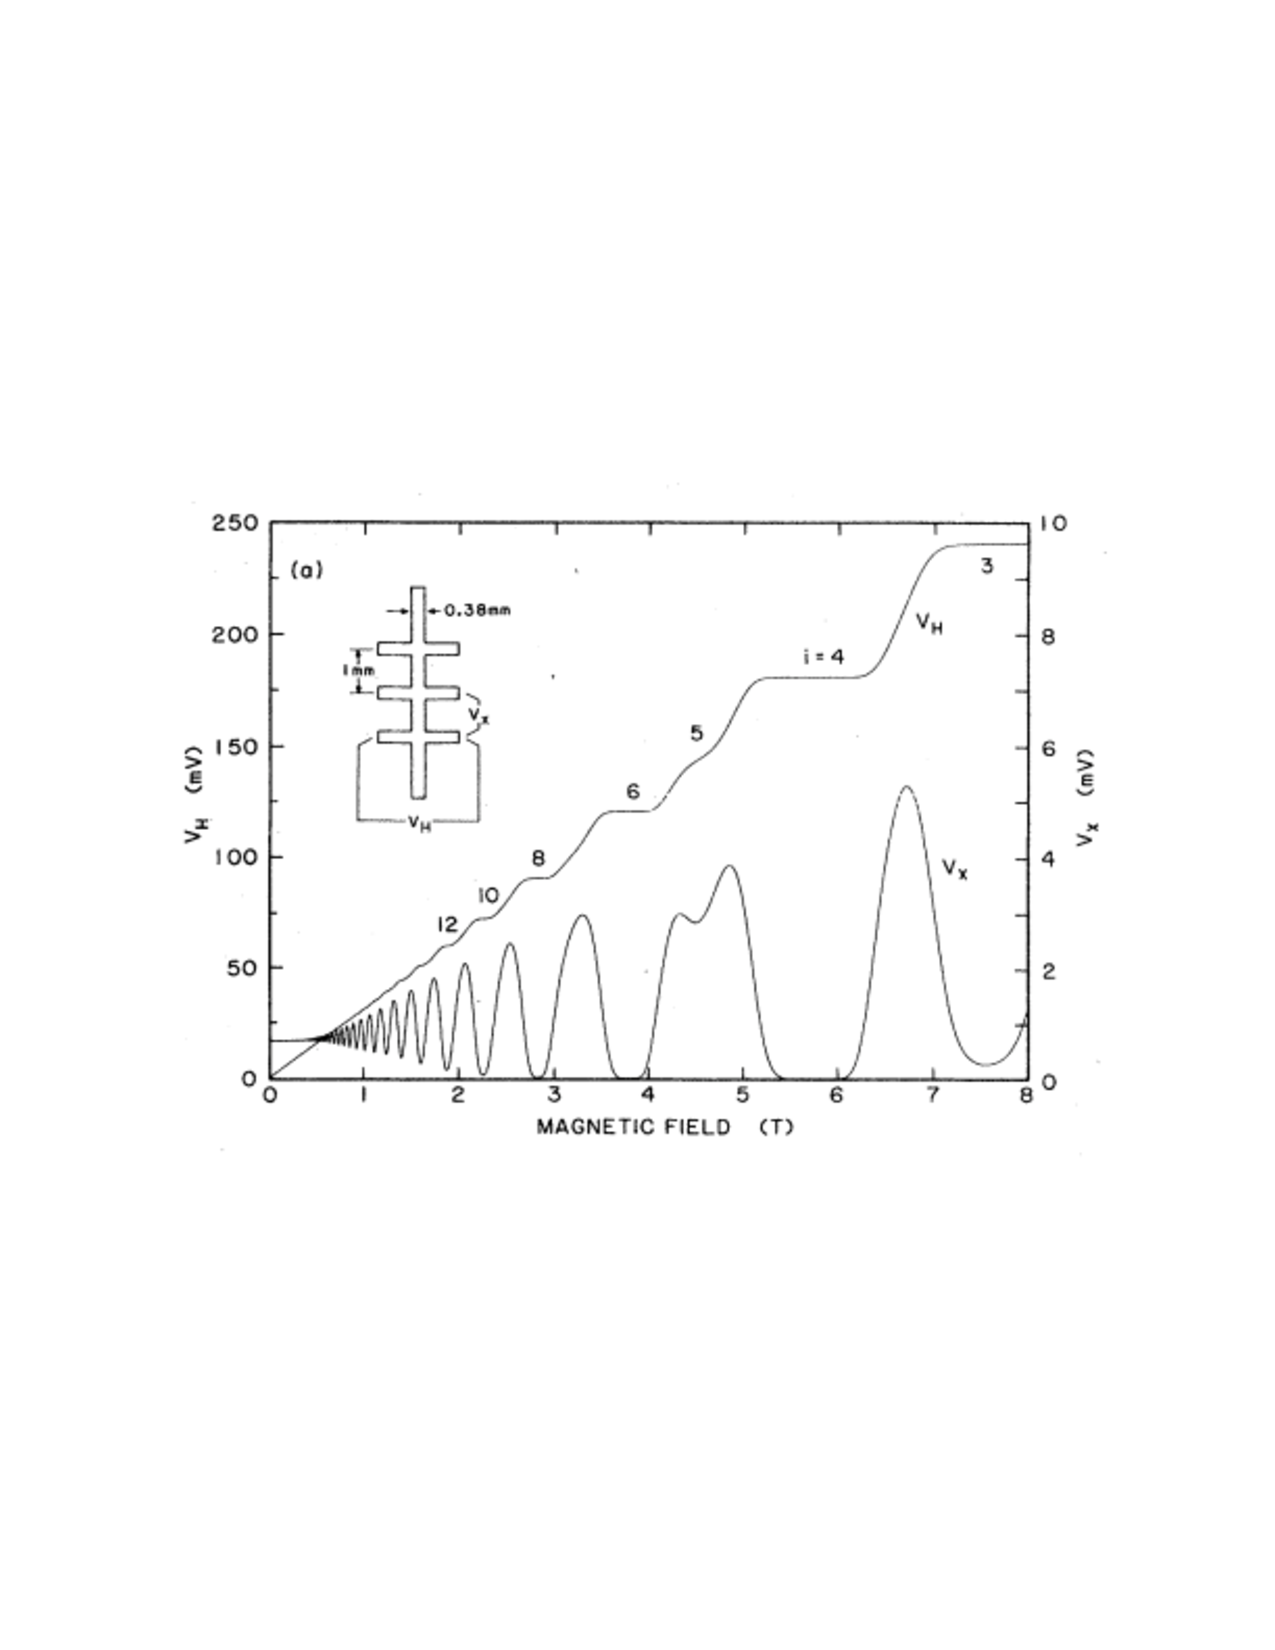
\includegraphics[width=10cm, angle=0]{ThesisCSULBLatexTemplate/figures/iqhe_plot_permission.pdf}
            \caption[The integer quantum Hall effect.]{The integer quantum Hall effect. Experimental data obtained from a GaAs heterostructure at $T=1.2$ K by Cage \textit{et al}. (1985). The Hall (transverse) resistivity sits on plateaus $\rho_{xy}=\frac{h}{e^2}\frac{1}{\nu}$ for a range of magnetic field values before suddenly jumping to the next plateau. The longitudinal resistivity, $\rho_{xx}$, vanishes at these plateaus before briefly spiking at each jump. Source: Reprinted with permission from Fig. 1 in  Ref. \cite{yennie}.}
            \label{iqhePlot}
            \end{center}
            \end{figure}
            
            These plateaus occur at
            \begin{equation} \label{iqhePlat}
            \rho_{xy}=\frac{h}{e^2}\frac{1}{\nu},
            \end{equation}
            where $\nu$ is measured to be an integer to one part per billion, and are centered around magnetic field strengths
            \begin{equation} \label{magFieldIqhe}
            B=\frac{h\rho}{\nu e}=\frac{\rho}{\nu}\phi_0.
            \end{equation}
            At low magnetic field strengths, the classical Hall effect is observed. However, when the electrons on the edges of the sample cannot complete their full cyclotron orbits, we often think of them as semiclassically bouncing around along the edges. This quenches the longitudinal resistance until the magnetic field reaches values where the edge orbits can be completed. At these magnetic field values, the Hall resistance jumps to a new plateau because the filling factor has decreased by one since the increased LL spacing has pushed the highest occupied LL above the Fermi energy~\cite{tong}. We can now explore what it means to be at a fractional filling factor.

        \subsection{Fractional Quantum Hall Effect}\label{ssec:fractQuantHallEff}\\
		
            Physicists found that as they decreased the sample disorder by trying other materials, lowering the temperature, and increasing the magnetic field strength, new plateaus in the Hall resistance became prominent. In 1982, Tsui \textit{et al}. were provided with a pure enough GaAs/AlGaAs semiconductor heterostructure sample to observe a plateau in the Hall resistivity at $\nu=1/3$ \cite{tsui}. Since then, over 70 rational fraction filling factors, $\nu=p/q$ for $p,q\in\mathbb{N}$, have been measured. A plot of this fractional quantum Hall effect (FQHE) can be seen in Fig. \ref{fqhePlot}.
		
		\begin{figure}[H]
            \begin{center}
            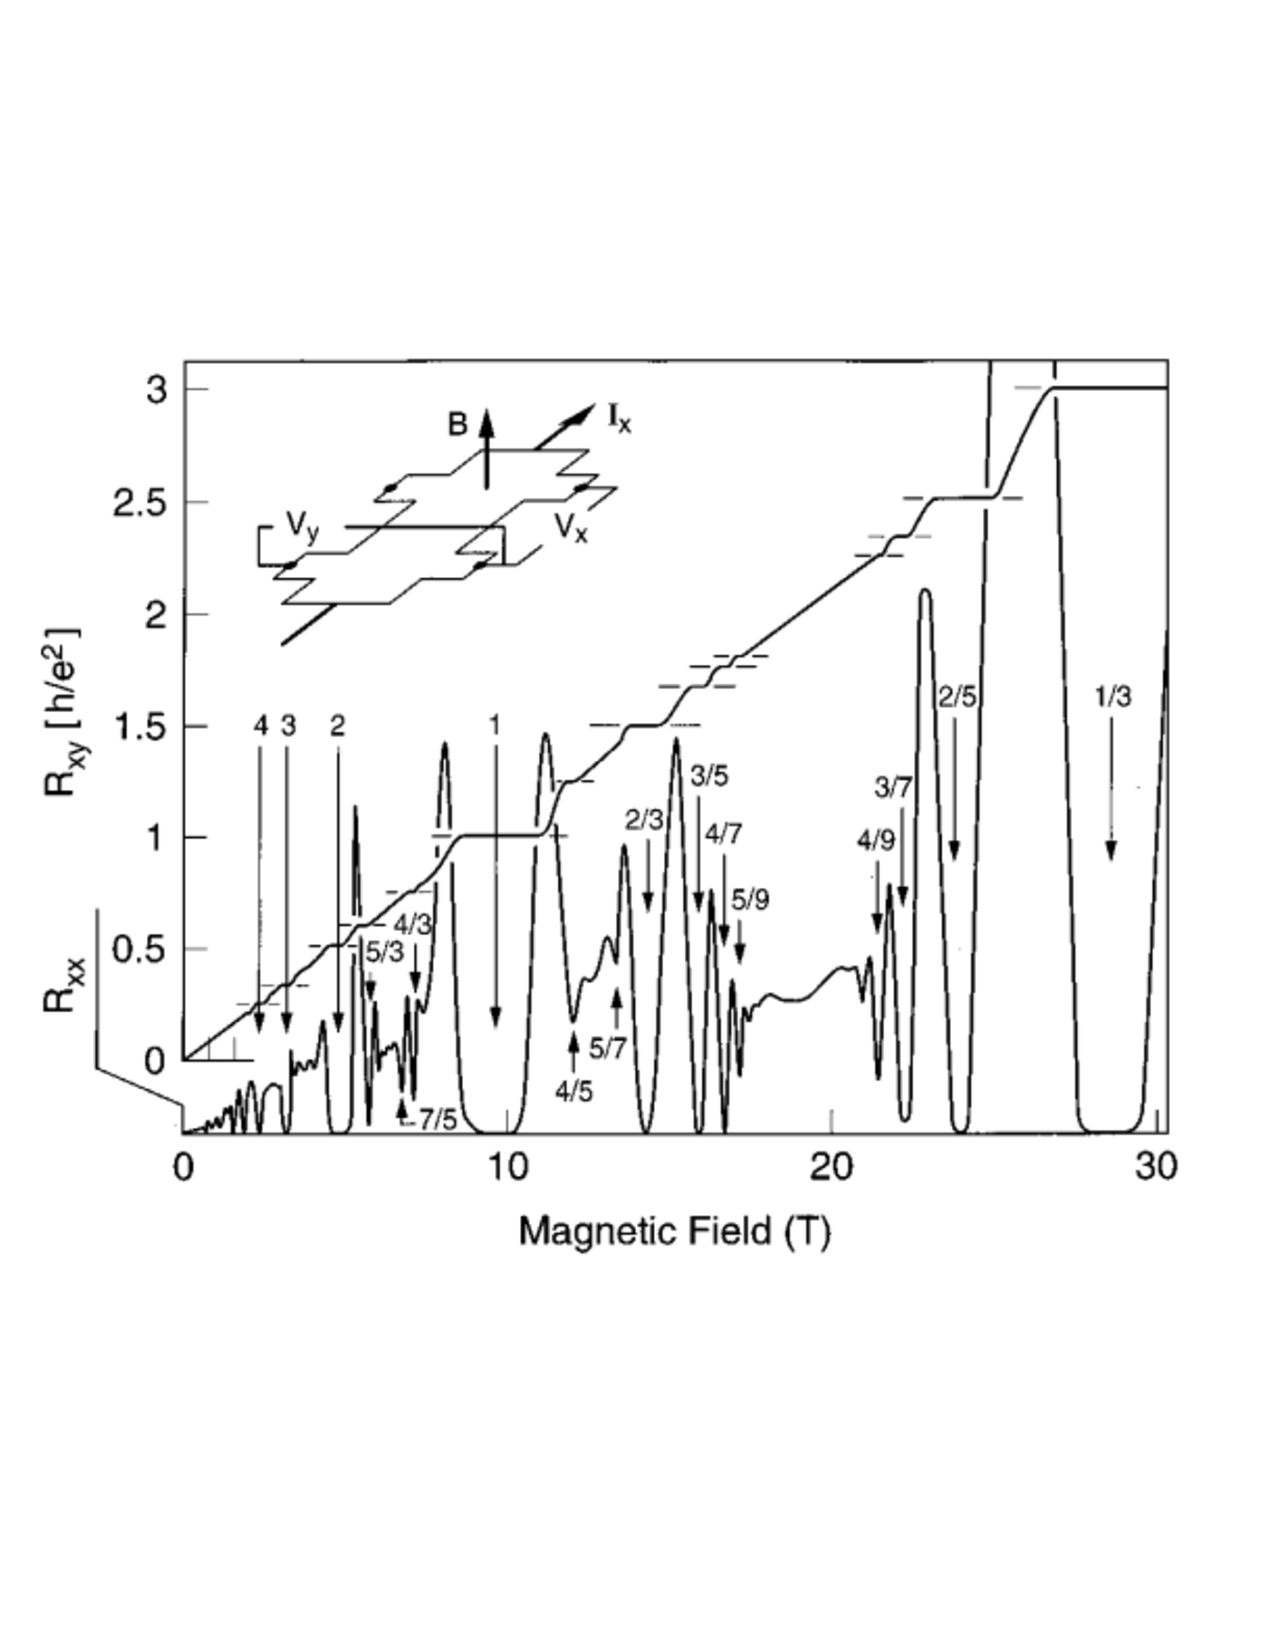
\includegraphics[width=10cm, angle=0]{ThesisCSULBLatexTemplate/figures/fqhe_plot.pdf}
            \caption[The fractional quantum Hall effect.]{The fractional quantum Hall effect. Experimental data obtained from a GaAs/AlGaAs heterostructure at $T=85$ mK by Eisenstein \textit{et al}. (1990). Like in the IQHE, the longitudinal resistance spikes at plateaus in the Hall resistance at $\rho_{xy}=\frac{h}{e^2}\frac{1}{\nu}$. However, this takes place at magnetic field strengths that correspond to rational fraction filling factors $\nu=\frac{p}{q}$, where $p,q\in\mathbb{N}$. Source: Reprinted with permission from Fig. 1 in Ref. \cite{stormer}.} 
            \label{fqhePlot}
            \end{center}
            \end{figure}
            
            As discussed in the previous section, the IQHE can be understood theoretically as an effect propagated by free electrons confined to two dimensions in a strong magnetic field, but Laughlin worked out that the Coulomb interactions between electrons must be taken into account to model the FQHE. It is then a many-body problem with Hamiltonian
            \begin{eqnarray}
                H = \sum_i \frac{\mathbf{\Pi}_i^2}{2m_b} + \sum_{i<j} \frac{e^2}{\epsilon l_B |\mathbf{r}_i-\mathbf{r}_j|} + \sum_i U(\mathbf{r}_i) + g\mu_B \mathbf{B}\cdot\mathbf{S},
            \end{eqnarray}
            where $\epsilon$ is the dielectric constant of the background material, $\mathbf{r}_i$ is the position of the $i^{th}$ electron, $U(\mathbf{r}_i)$ is a single particle potential (e.g. a confining potential), $g$ is the Land\'e g-factor, $\mu_B$ is the effective Bohr magneton, and $\mathbf{S}$ is the total spin of the electrons in the system. If we neglect $U(\mathbf{r}_i$), which amounts to a constant energy shift, and assume the electrons are fully polarized by the strong magnetic field, then the Hamiltonian becomes 
            \begin{eqnarray}
                H &=& \sum_i \frac{\hbar\omega_B}{2}(n_i + 1) + \sum_{i<j} \frac{e^2}{\epsilon l_B |\mathbf{r}_i-\mathbf{r}_j|}\;.
            \end{eqnarray}
            The kinetic energy term has vanished and the highest occupied LL is only fractionally filled for a rational fraction filling factor $\nu$. The electrons in the fractionally filled LL are degenerate, requiring a full solution of their Coulomb interactions - providing a difficult challenge for theorists. For these calculations, numerical approaches are used, including exact diagonalization of finite sized systems, Monte Carlo (MC) methods, and more recently, the density matrix renormalization group (DMRG).
            
            Laughlin published the following wave function for the ground state at filling factor $\nu=1/m$:
            \begin{equation}\label{eqn:one_over_m_wavefnx}
            \Psi_{1 / m}=\prod_{j<k}\left(z_{j}-z_{k}\right)^{m} \mathrm{e}^{-\frac{1}{4} \sum_{i}\left|z_{i}\right|^{2}},
            \end{equation}
            where $m$ is an odd integer to preserve antisymmetry and $z_j=x_j-iy_j$ are the coordinates of the j$^{th}$ electron in the complex plane using the symmetric gauge, $\mathbf{A} = B(-y,x,0)/2$. Through a series of arguments, he showed that this state, $\Psi_{1/m}$, describes a uniform density incompressible ground state with a finite energy gap which would experimentally manifest as a plateau in the Hall resistance at $\rho_{xy} = h/e^2(1/m)$. In addition, he worked out that the low energy excitations of these states have an electric charge of magnitude $e/m$ \cite{jain}.
            These excitations also obey Abelian fractional statistics, which can be found in the continuous range  between Fermi-Dirac and Bose-Einstein statistics \cite{laughlin}. The experimental demonstration of non-Abelian fractional statistics, which might occur in systems such as the FQHE at $\nu=5/2$ in GaAs heterostructures, could be the key step in building a topologically protected quantum computer \cite{nayak}. To explain filling factors other than those coming from Laughlin's wavefunction, however, we require composite fermion theory.
    		
\section{Composite Fermions}\label{sec:compFerm}

	Understanding the strongly-interacting electron problem directly proved to be difficult, but in 1989 Jain noticed that if the numbers on the plot of the FQHE (Fig.~\ref{fqhePlot}) were erased, it would be indistinguishable from the plot of the IQHE (Fig.~\ref{iqhePlot}). He used this insight to successfully  reformulate the FQHE in terms of noninteracting quasiparticles called composite fermions (CFs). The rest of this section will provide a brief introduction to this concept that follows from Jain's textbook \textit{Composite Fermions}~\cite{jain}.
	
	In CF theory, strongly-interacting electrons at filling factor $\nu$ in the lowest Landau level (LLL) are recast as functions of noninteracting (or weakly interacting) CFs that occupy Landau-like $\Lambda$ levels at CF filling factor $\nu^*$. The relationship between the electron and CF filling factors is given by
	\begin{equation} \label{compFermFill}
    \nu=\frac{\nu^*}{2p\nu^*\pm1},
    \end{equation}
    where $p\in\mathbb{N}_0$ and the minus sign in the denominator occurs when the effective magnetic field vector points opposite the external magnetic field vector. The CF wavefunction is given by
    \begin{equation} \label{compFermEigFunct}
    \Psi_\nu=\mathcal{P}_{LLL}\prod_{j<k}(z_j-z_k)^{2p}\Phi_{\nu^*},
    \end{equation}
    where $\Phi_{\nu^*}$ is the noninteracting electron wave function and $\mathcal{P}_{LLL}$ projects the state onto the lowest Landau level. CFs are the bound state between the noninteracting electrons in $\Phi_{\nu^*}$ and the $2p$ quantum vortices attached to them by the Jastrow factor,
    \begin{equation}\label{eqn:jastr_fact}
    \prod_{j}\mathcal{J}^p_j=\prod_{j<k}(z_j-z_k)^{2p}.
    \end{equation}
    
    The Berry phase of the attached vortices cancel the Aharanov-Bohm phase that arises as the CFs move about in the presence of an external magnetic field. Therefore, CFs exist in the reduced effective magnetic field $B^*$ at the mean-field level, 
    \begin{equation} \label{compFermMagnField}
    B^*=B-2p\rho\phi_0,
    \end{equation}
    where the electron and CF density $\rho$ is the same. If $\nu^*=n$ for $n\in\mathbb{N}$, it is reasonable to expect an energy gap to exist due to the $n$ filled $\Lambda$-levels, and therefore the CFs would manifest as plateaus centered around $B^*=(\rho/\nu^*)\phi_0$, analogous to the IQHE for electrons. This would then correspond to the FQHE of electrons for electron filling factor
    \begin{eqnarray}
        \nu = \frac{n}{2pn\pm 1},
    \end{eqnarray}
    which is precisely the values for most experimentally observed FQHE plateaus. 
    
    The energy expectation value for a FQH system at electron filling factor $\nu$ is 
    \begin{equation} \label{compFermEigEn}
    E_\nu=\frac{\braket{\Psi_\nu|\sum_{j<k}\frac{1}{r_{jk}}|\Psi_\nu}}{\braket{\Psi_\nu|\Psi_\nu}}+V_{el-bg}+V_{bg-bg}, 
    \end{equation}
	where $V_{el-bg}$ is the electron-background interaction energy, $V_{bg-bg}$ is the background-background interaction energy, and we are assuming there is a uniformly positively charged background such that the charge of the system is neutralized. The CF energy gaps are calculated via the CF-exciton ($\Delta$) dispersion. Excitons are CF-quasiparticle and CF-quasihole pairs created by the promotion of a CF to an unoccupied $\Lambda$ level. They are calculated as the difference between the ground state energy and the lowest energy of the state with a given total angular momentum, $L$. The CF-rotons ($\Delta_r$) are the minima of the exciton dispersion and can be measured experimentally via inelastic Raman scattering. The transport gap ($\Delta_t$), also referred to as the activation energy in the literature, is the energy required to create a quasiparticle and quasihole pair separated far enough to move independently, therefore contributing to transport. It converges to a constant value as the number of electrons increases, which can be measured experimentally via the longitudinal resistance as a function of the temperature. A schematic diagram of the exciton dispersion can be seen in Fig. \ref{transpGapDisp}. There exist energies above the line drawn on the plot, but we are only interested in visualizing the gap from the ground state to the lowest energy excitation at each wave vector $kl=L/\sqrt{Q}$. Analytical calculations of FQH energies require reformulating the problem in terms of Haldane pseudopotentials, which we will discuss in the next section.

    \begin{figure}[h]
    \begin{center}
    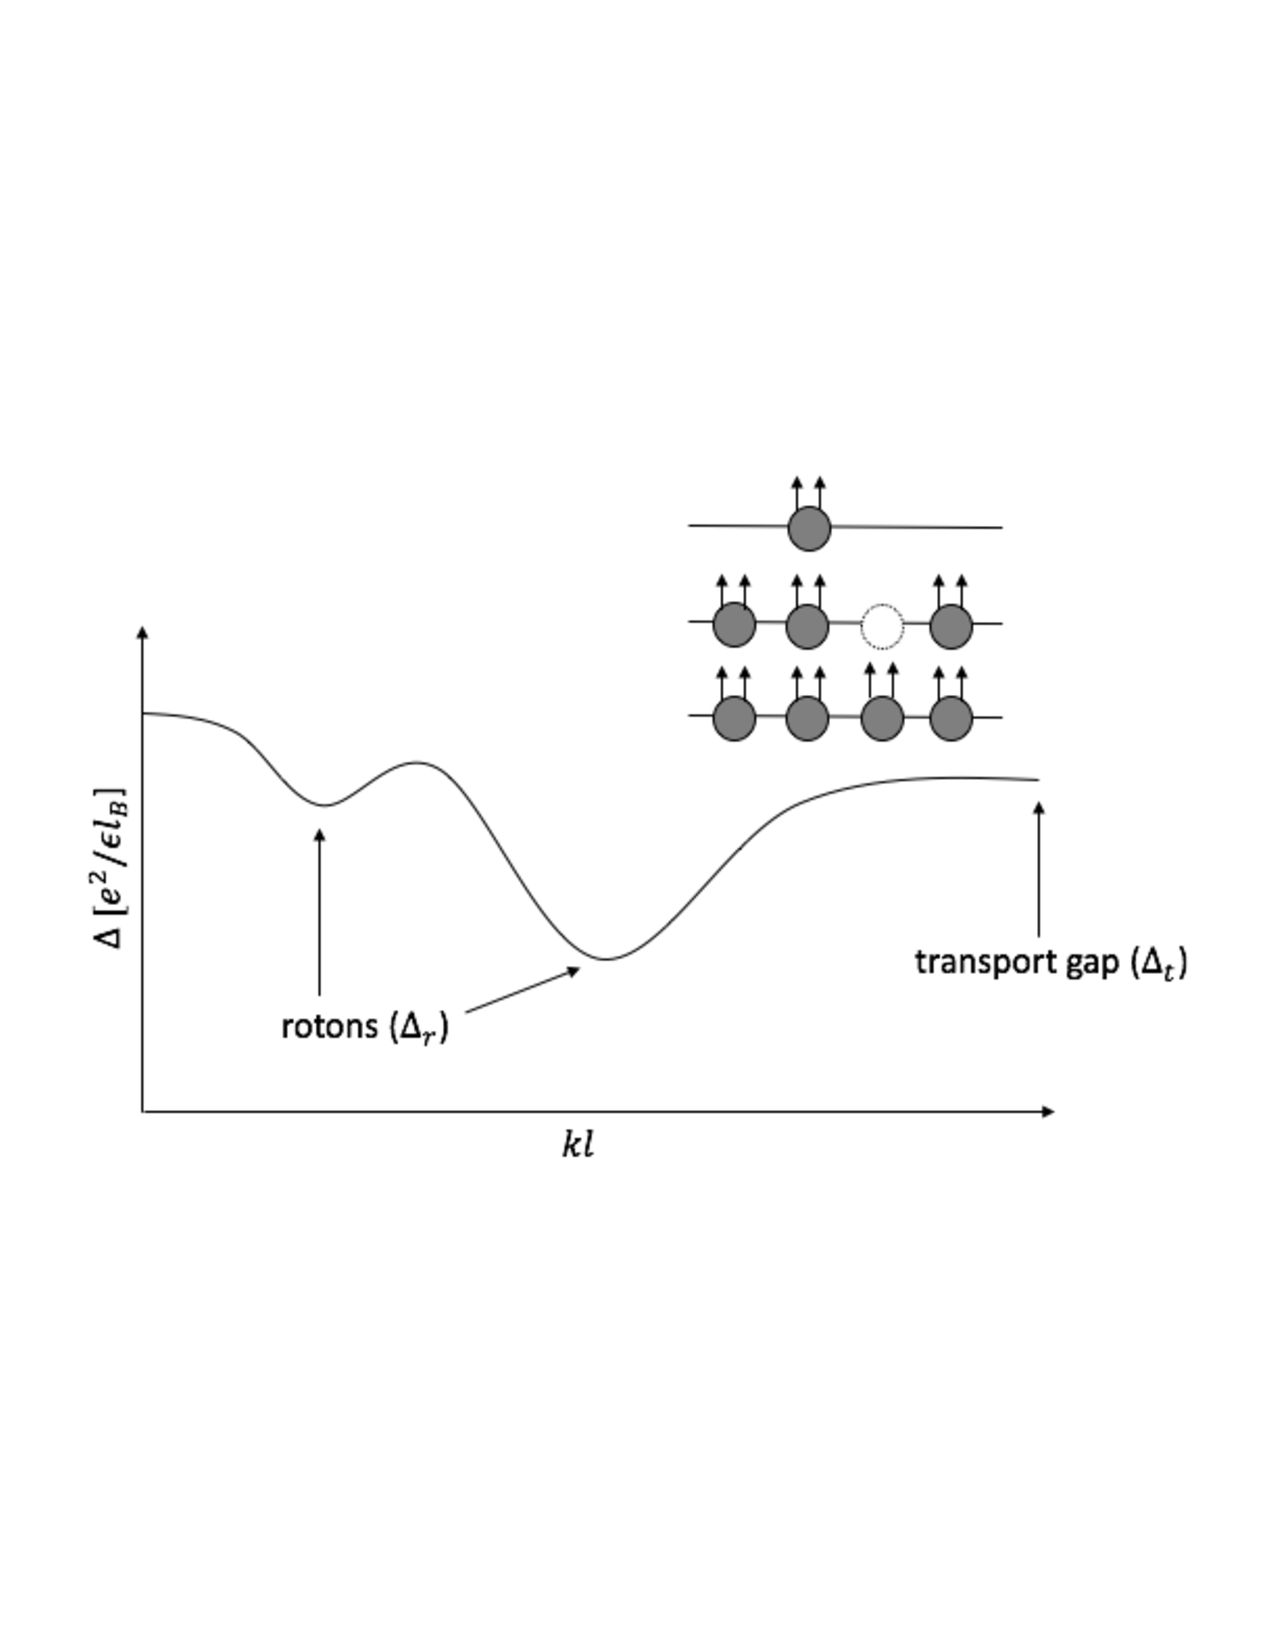
\includegraphics[width=10cm, angle=0]{ThesisCSULBLatexTemplate/figures/cf_exciton_drawing.pdf}
    \caption[The low energy composite fermion-exciton dispersion.]{The low energy composite fermion-exciton dispersion. Excitons ($\Delta$) are created by promoting a CF to an unoccupied $\Lambda$ level (inset). The rotons ($\Delta_r$) are the local minima of the dispersion. At large wave vectors $kl$, the dispersion converges to the transport gap ($\Delta_t$), where the quasiparticle and quasihole pair are separated far enough to move independently. The plotted line represents the gap between the ground state and the lowest energy excitation for each wave vector.}
    \label{transpGapDisp}
    \end{center}
    \end{figure}

    \section{Haldane Pseudopotentials}\label{sec:haldPseud}
    The FQHE is a challenging many-body problem, requiring theorists to solve the fully interacting Hamiltonian 
    \begin{eqnarray}
        H &=& \sum_{i<j} \frac{e^2}{\epsilon l_B |\mathbf{r}_i-\mathbf{r}_j|}\;,
    \end{eqnarray}
    where we have neglected the kinetic energy term. In 1983, Haldane introduced a useful parameterization of the interacting FQHE Hamiltonian in terms of so-called Haldane pseudopotentials (PPs) \cite{haldane}. Very generally, the Hamiltonian can be rewritten as
    \begin{eqnarray}\label{HamPPexpand}
        H &=& \sum_{i<j} \frac{e^2}{\epsilon l_B |\mathbf{r}_i-\mathbf{r}_j|}\nonumber\\
        &=& \sum_m V^{(n)}_m \sum_{i<j} P_{ij}(m),
    \end{eqnarray}
    where $m$ is the relative angular momentum between the $i^{th}$ and $j^{th}$ electrons, $P_{ij}(m)$ is a projection operator for a state with relative angular momentum $m$, and $V^{(n)}_m$ are the Haldane pseudopotentials. The PP represents the interaction energy between two electrons confined to the $n^{th}$ LL with relative angular momentum $m$. They are a useful parameterization because, for a given interaction potential, they completely determine the problem and significantly simplify numerical approaches such as exact diagonalization.
    
    In this thesis, we utilize Haldane's spherical geometry where the two-dimensional plane is mapped to the boundary free surface of a sphere of constant radius $R=\sqrt{Q}l_B$. The perpendicular magnetic field becomes a radial magnetic field emanating from a magnetic monopole in its center with strength $Q$ (see Fig.~\ref{fig:haldSpher}). Mapping this problem to the spherical geometry mitigates complications that arise from edge effects. In 1976, Tai Tsun Wu and Chen Ning Yang solved for the wavefunction of a charged particle moving in the presence of a Dirac monopole \cite{wu}. The single particle eigenstates in the spherical geometry are the monopole harmonics
	\begin{equation} \label{monHarm}
    Y_{q,n,m}(\Omega)=N_{qnm}2^{-m}(1-x)^{\frac{-q+m}{2}}(1+x)^{\frac{q+m}{2}}P_{q+n-m}^{-q+m,q+m}(x)e^{i(q-m)\phi},
    \end{equation}
    where $N_{qnm}$ is the normalization coefficient
    \begin{equation} \label{monHarmNormCo}
    N_{qnm}=\left(\frac{(2q+2n+1)}{4\pi}\frac{(q+n-m)!(q+n+m)!}{n!(2q+n)!}\right)^{1/2},
    \end{equation}
    the total flux through the sphere is $2q\phi_0$ for $2q\in\mathbb{Z}$, $m=-q-n,-q-n+1,...,q+n$ are the degenerate states in the $n^{th}$ LL, $l=q+n$ is the single particle angular momentum, $x=cos\theta$, and $P^{\alpha,\beta}_\gamma$ are the Jacobi polynomials \cite{bible}. 
    
    \begin{figure}[h]
    \begin{center}
    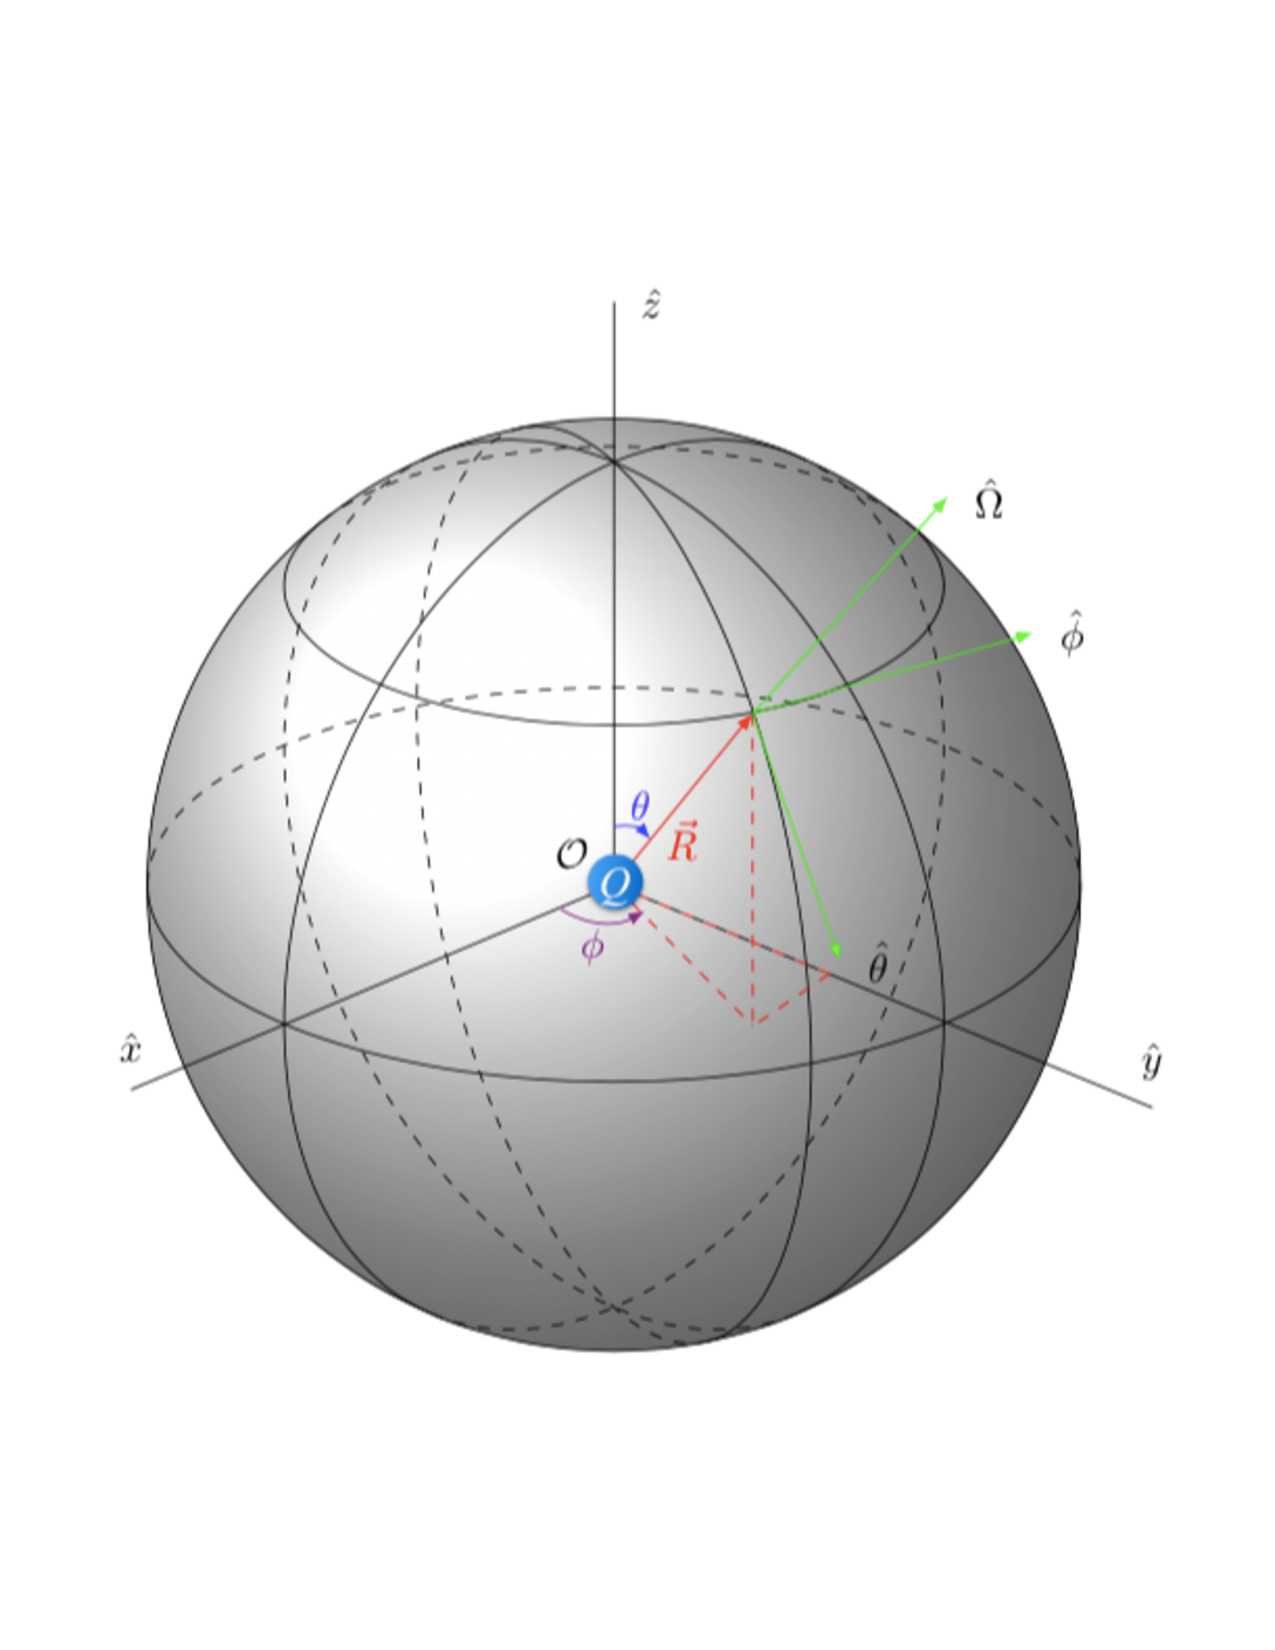
\includegraphics[width=10cm, angle=0]{ThesisCSULBLatexTemplate/figures/haldane_sphere_thesis.pdf}
    \caption[The Haldane sphere.]{The Haldane sphere. The 2D electron gas is mapped to the surface of a sphere of radius $R=\sqrt{Q}l_B$ to mitigate complications arising from edge effects. The perpendicular magnetic field emanates from a magnetic monopole of strength $Q$ in the sphere's center. Source: Reprinted with permission from Fig. 1 in  Ref.~\cite{arciniaga}.}
    \label{fig:haldSpher}
    \end{center}
    \end{figure}
    
    \vspace{4pt} % keep uniform double spacing below caption
    
    The MC code we use to calculate the exciton dispersion requires a real space potential to calculate the interaction energies between electrons on the Haldane sphere. We will be incorporating realistic material effects into the PPs, which have no explicit form in real space since the mapping between real space and the spherical geometry is not bijective. Therefore, we need to use an effective potential in real space that can reflect the changes realistic effects make to the bare Coulomb PP. In her 2013 doctoral dissertation, Rachel Wooten published a scheme for mapping an effective real space potential to a PP in the spherical geometry. The $n^{th}$ LL PP,
    \begin{equation} \label{wootPpNthLl}
    V_{l,Q}=\braket{Q,l,l;L,M|V(|r_{12}|)|Q,l,l;L,M},
    \end{equation}
    is given in Coulomb units by
    \begin{equation} \label{wootPp}
    V_{l,Q}(L)=\frac{1}{\sqrt{Q}}\sum_{k=0}^{2l}V_k(-1)^{2Q+L}(2l+1)^2
    \begin{Bmatrix}
    L & l & l\\
    k & l & l
    \end{Bmatrix}
    \begin{pmatrix}
    l & k & l\\
    -Q & 0 & Q
    \end{pmatrix}
    ^2,
    \end{equation}
    where $l=|Q|+|n|$ is the single-particle angular momentum, $L=2l-m$ is the two-body relative angular momentum in the spherical geometry,
    \begin{equation} \label{wootPpVk}
    V_k=\frac{1}{2}\int_0^\pi V(r_{12})P_k(\cos\theta)\sin\theta d\theta,
    \end{equation}
    $V(r_{12})$ is the effective two-dimensional interaction, $P_k(cos\theta)$ are the Legendre polynomials, the curly bracket matrix contains Wigner's 6-j symbols, and the round bracket matrix contains Wigner's 3-j symbols~\cite{wooten}. Plugging an effective interaction $V(r_{12})$ into this expression yields its corresponding PP in the spherical geometry as a function of the relative angular momentum, $V_{l,Q}(L)$. We work with PPs in the spherical geometry since it is more amenable to the addition of realistic effects. However, solving for the energies in terms of PPs in the spherical geometry via exact diagonalization requires an expansion of Slater determinant basis states which makes calculations impractical for systems with larger than $\sim10$ electrons. For this reason, we instead approximate the energies via a variational Monte Carlo (MC) method (see Sec.~\ref{ssec:montCarlInt} for more details). This MC method, however, requires a real space potential, so we incorporate realistic effects into our energy calculations by mapping the real space potential (to be used in the MC calculation) to a realistic effect-incorporated PP in the spherical geometry via Wooten's method.
    
    A popular choice in the literature for a real space potential for MC calculations is the Park potential. Park $\textit{et al.}$ investigated the mysterious even-denominator FQH state at $\nu=5/2$, where the CF filling factor of the first-excited LL is $\nu^*=1/2$. They devised the following effective interaction in the LLL (in units of $e^2/\epsilon l_B$) to produce the same PPs as the Coulomb interaction in the first-excited LL:
    \begin{equation} \label{parkPot}
    V_{eff}(r)=\left(\frac{1}{r}+a_1e^{-\alpha_1r^2}+a_2r^2e^{-\alpha_2r^2}\right)\left[\frac{e^2}{\epsilon l_B}\right],
    \end{equation}
    where the distance $r$ is in units of effective magnetic length $l_{B^*}=(\hbar/eB^*)^{1/2}$, the fitting parameters $\{a_1,a_2,\alpha_1,\alpha_2\}$ are calculated by fitting the first four significant PPs exactly, $\epsilon$ is the dielectric constant of the background material, and $l_B=\sqrt{\frac{\hbar}{eB}}$ is the magnetic length at actual electron filling factor $\nu$. The first four significant PPs are those for which $m\in\{1,3,5,7\}$ - they are odd because the many-body wavefunction has to be fully anti-symmetric under particle exchange for fermions, and since in the planar geometry $m$ is directly proportional to the chord distance between electrons $r$ in the potential $V(r)$, the first four sample the strongest Coulomb interactions \cite{park}. We will be fitting a modified version of the Park potential to PPs that incorporate realistic effects into the spherical geometry via Wooten's formula (see Sec.~\ref{ssec:realSpaceEffPot}). The first realistic effect we want to benchmark our method against, LLM, can be quenched in the $B\rightarrow\infty$ limit for GaAs/AlGaAs semiconductor heterostructures, but not in the material graphene, which we will discuss in the next section.

    \section{Graphene}\label{sec:graph}
    In 2004, Novoselov \textit{et al}. developed a simple way to isolate graphene, an atomically-thin hexagonal carbon lattice, using regular adhesive tape \cite{novoselov}. The next year, Novoselov \textit{et al}. found that the electrons and holes in graphene obey a linear dispersion, appropriate for massless particles. In this case, the Fermi velocity $\nu_F$ is approximately $10^6$ m/s \cite{novoselov2005}. In 2009, both Du \textit{et al}. and Bolotin \textit{et al}. separately manufactured pure enough samples of suspended graphene to observe the FQHE at $\nu=1/3$ \cite{du,bolotin}. The next year, Skachko \textit{et al}. measured a clear plateu in the Hall resistivity at $\nu=1/3$ in temperatures ranging from 2 K to up to 20 K in a 12 T external magnetic field. The charge carrier density, which corresponds to the filling factor $\nu$, can be adjusted in graphene at a constant magnetic field via the gate voltage $V_g$ \cite{skachko}. In 2015, Amet \textit{et al}. demonstrated the FQHE in other filling factors of graphene, $\nu=\frac{p}{2p\pm1}$, where $p$ is an integer less than or equal to 5 \cite{amet}. A plot of the FQHE in graphene can be seen in Fig. \ref{fqheGraph}.
	
    \begin{figure}[H]
    \begin{center}
    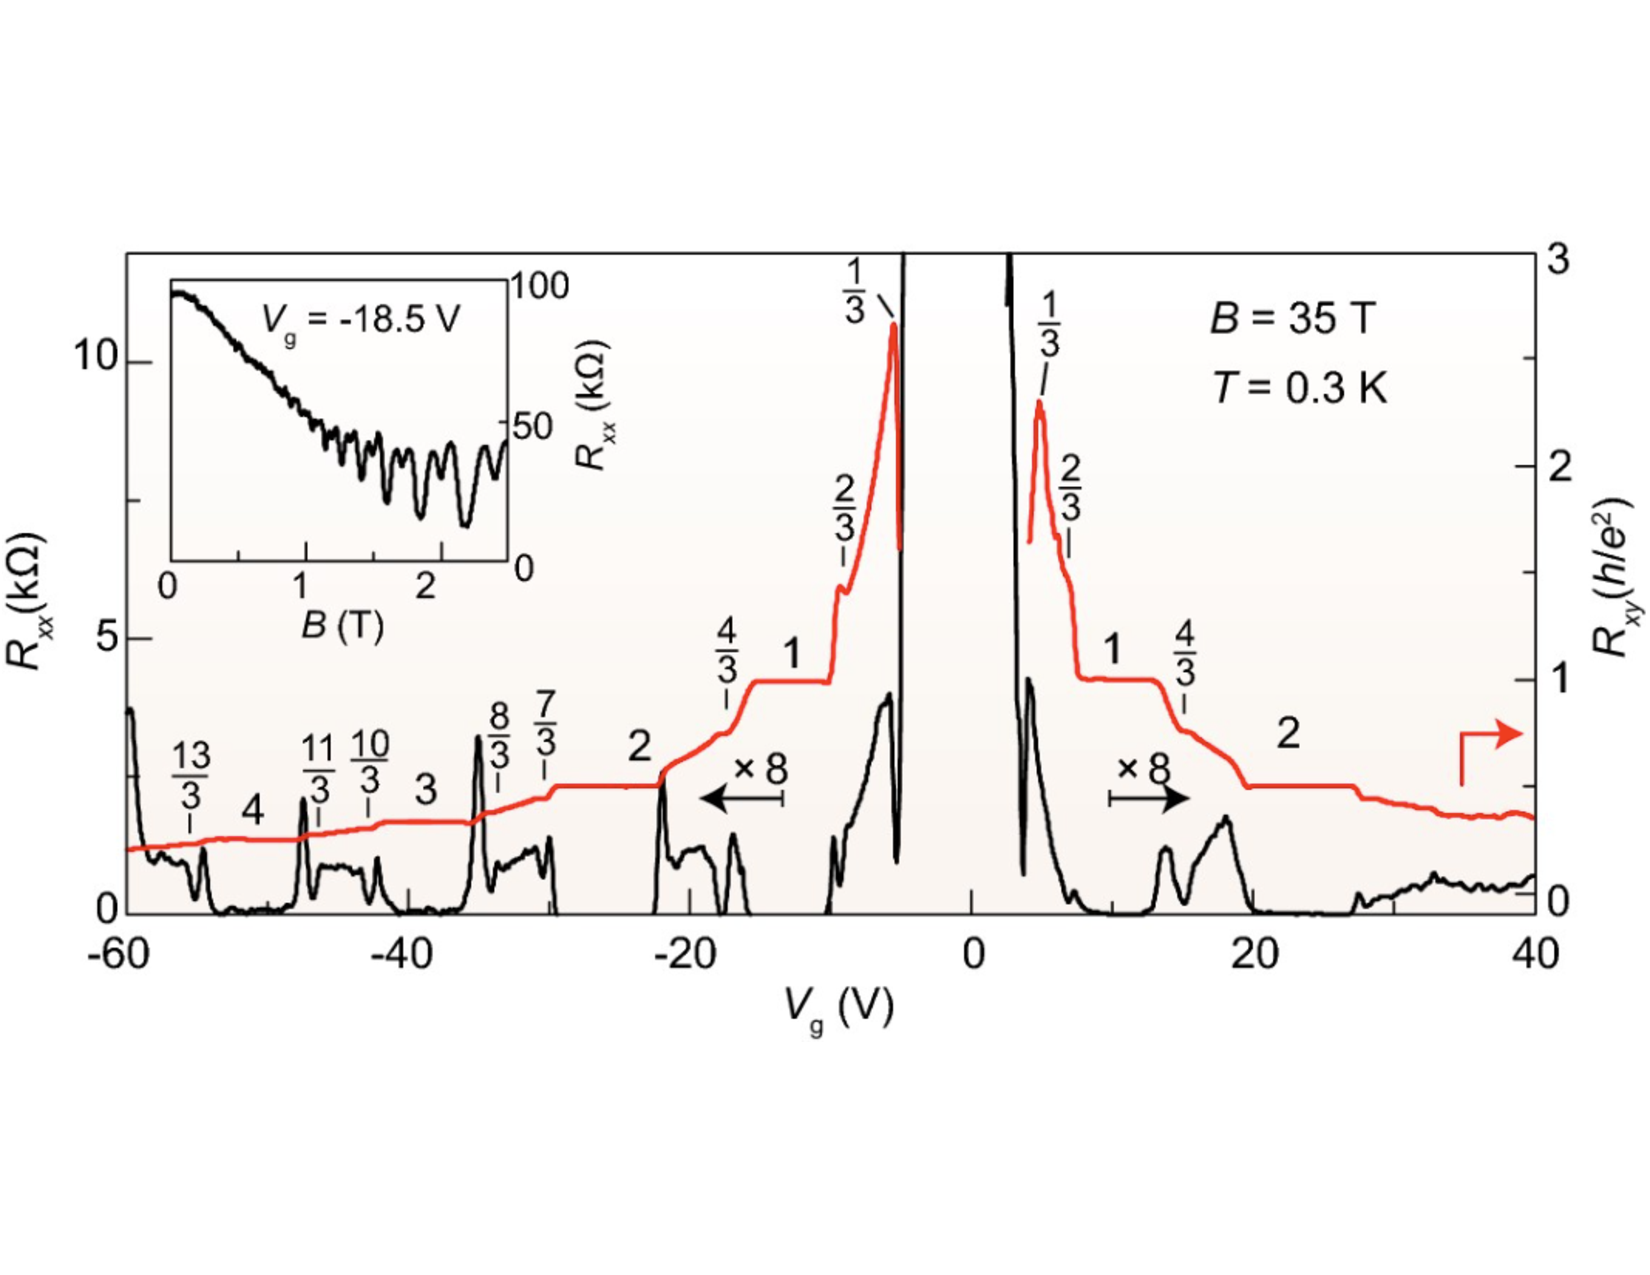
\includegraphics[width=10cm, angle=0]{ThesisCSULBLatexTemplate/figures/fqhe_graphene.pdf}
    \caption[The FQHE in graphene.\vspace{-12pt}]{The FQHE in graphene. Experimental data obtained from graphene at $T=0.3$ K by Dean \textit{et al.} (2011). In graphene, the gate voltage $V_g$ can be used to adjust the filling factor $\nu$ at a constant magnetic field strength (i.e. $B=35$ T). Source: Adapted from Fig. 13 in Ref. \cite{lin}.}
    \label{fqheGraph} 
    \end{center}
    \end{figure}
    
    For free electrons in graphene, there are two Fermi points $K$ and $K^\prime$, each with a two-fold band degeneracy (from the $A$ and $B$ sublattice). The continuum Hamiltonian for one pseudospin component is 
    \begin{eqnarray}
    H &=& \nu_F \mathbf{\sigma}\cdot \mathbf{\Pi}\\
    &=& \nu_F \begin{pmatrix}
    0 & \Pi_x - i \Pi_y\\
    \Pi_x + i\Pi_y & 0
    \end{pmatrix}\;,
    \end{eqnarray}
    where $\mathbf{\sigma} = (\sigma_1, \sigma_2, \sigma_3)$ are the Pauli matrices and $\mathbf{\Pi}$ is the canonical momentum defined in Eq.~\ref{eq:can_mom}. The following is adapted from Refs.~\cite{arciniaga, apalkov, goerbig, toke, nomura, Toke2007}. Reintroducing the ladder operators from before, we get the Hamiltonian
    \begin{eqnarray}
    H&=& \nu_F\frac{\hbar\sqrt{2}}{l_B} \begin{pmatrix}
    0 & a \\
    a^\dagger & 0
    \end{pmatrix}\;.
    \end{eqnarray}
    The standard way to solve this Hamiltonian is to instead consider its square, 
    \begin{eqnarray}
    H^2 &=& \nu_F^2\frac{2\hbar^2}{l_B^2} \begin{pmatrix}
    aa^\dagger & 0 \\
    0 & a^\dagger a
    \end{pmatrix}\;,
    \end{eqnarray}    
    which is simpler because $[a,a^\dagger]=1$ and $a^\dagger a=n$ is the number operator. The eigenfunctions of $H^2$ can be found to be 
    \begin{eqnarray}
        \psi_{nm}(x,y) = \frac{(\sqrt{2})^{\delta_{n0}}}{\sqrt{2}}
        \begin{pmatrix}
        -\mathrm{sgn}(n) i \eta_{|n|-1,m}(x,y) \\
        \eta_{|n|m}(x,y)
        \end{pmatrix},
    \end{eqnarray}
    where $\eta_{nm}(x,y)$ are the single-particle eigenfunctions of the quadratic energy dispersion for massive fermions. Since $[H,H^2]=0$, the two Hamiltonians share common eigenfunctions and the energy spectrum can be found to be
    \begin{eqnarray} \label{eqn:graphSpectr}
        E_n &=& \frac{\hbar \nu_F}{l_B} \sqrt{2|n|}\;.
    \end{eqnarray}
    This different spectrum and eignenstate structure augments the PPs for the FQHE in graphene. However, it can essentially be expressed in terms of combinations of the massive electron result for semiconductor heterostructures given in Eq.~\ref{wootPpNthLl} (see Arciniaga and Peterson for more details~\cite{arciniaga}). The linear electron dispersion and energy spectrum given in Eq.~\ref{eqn:graphSpectr} create a unique LL structure for graphene. The spacing between energy eigenvalues in a GaAs/AlGaAs semiconductor heterostructure remained constant as a function of the cyclotron energy $\hbar\omega_B$, but in graphene, the LLs clump together as the space between their energies decreases at larger LL indices $n$. This creates problems for theorists using traditional methods to calculate the CF exciton dispersion for graphene because there is then no magnetic field strength that can quench the effects of Landau level mixing, which we will discuss in the next section.
	
	\subsection{Landau Level Mixing} \label{ssec:landLevMix}
	    In 2006, T\ifmmode \mbox{\H{o}}\else \H{o}\fi{}ke \textit{et al}. calculated the transport gaps for FQH states of graphene at filling factor $\nu\in\{1/3,2/5\}$ \cite{toke}. However, theoretical predictions for measurable gaps have not yielded acceptable agreement with experiment. It is typical for these calculations to ignore Landau level mixing (LLM), an effect that arises when Coulomb interactions push electrons into higher LLs, or alternatively, holes into lower LLs. It is characterized by the parameter $\kappa$, the ratio of the Coulomb energy to the cyclotron energy. One of the factors that makes these calculations unique for graphene is its linear, as opposed to parabolic, electron dispersion. This prevents the suppression of LLM by a sufficiently strong magnetic field via the following relation from Ref. \cite{peterson2014}:
        \begin{equation} \label{kappGraph}
        \kappa = 
        \begin{cases} 
        \frac{e^2/\epsilon l_B}{\hbar\omega_B} \sim \frac{2.5}{\sqrt{B[\text{tesla}]}}, & \text{GaAs semiconductor} \\
        \frac{e^2/\epsilon l_B}{\hbar\nu_F/l_B} = \frac{e^2}{\epsilon\hbar\nu_F}=\frac{2.2\text{ (Kelvin)}}{\epsilon}, & \text{graphene.}
        \end{cases}
        \end{equation}
        The experimental value of $\kappa$ depends on the substrate the sample rests upon. For a suspended graphene sample $~{\kappa}\approx2.2$, for graphene on a SiO$_2$ substrate $~{\kappa}\approx0.9$, and for a boron nitride substrate $~{\kappa}\approx0.5-0.8$ \cite{peterson}.
	    
	    Peterson \textit{et al}. developed a scheme for incorporating LLM effects into PPs via the following Hamiltonian \cite{peterson2014}:
        \begin{equation} \label{hamHaldSphere}
        \begin{split}
        H(\kappa) & = \sum_{i<j}V_{eff}(\kappa,|\mathbf{r}_i-\mathbf{r}_j|)+\sum_{i<j<k}V_{3body}(\kappa,\mathbf{r}_i,\mathbf{r}_j,\mathbf{r}_k) \\
        & = \sum_\alpha V_\alpha^{(2)}(N,\kappa)\sum_{i<j}\hat{P}_m(m_{ij}) + \sum_\beta V_\beta^{(3)}(N,\kappa)\sum_{i<j<k}\hat{P}_{ijk}(m_{ijk}),
        \end{split}
        \end{equation}
        where $\hat{P}_m(m_{ij})$ projects electrons $i$ and $j$ onto their respective angular momentum state $m_{ij}$, $\hat{P}_{ijk}(m_{ijk})$ projects electrons $i$, $j$, and $k$ onto $m_{ijk}$, and $V_\alpha^{(2)}(N,\kappa)$ and $V_\beta^{(3)}(N,\kappa)$ are the $\kappa$ dependent two and three-body effective PPs, respectively. For LLs $n\ge1$, LLM generates particle-hole symmetry breaking three-body terms, but in the LLL (which we confine ourselves to in this thesis), the three-body terms in Eq.~\ref{hamHaldSphere} vanish due to this symmetry \cite{peterson}. 
        
        In 2016, Arciniaga \textit{et al}. calculated perturbative corrections to the two-body PPs in the LLL, $\delta V^{(n=0)}_{2l-m}$, such that the corrected two-body PPs are given by
        \begin{equation} \label{potLlm}
        V^{(0)}_{2l-m,2body}(\kappa) = V^{(0)}_{2l-m} + \kappa\delta V^{(0)}_{2l-m},
        \end{equation}
        where $V^{(0)}_{2l-m}$ is the two-body bare Coulomb PP in the LLL \cite{arciniaga}. Then, in his master's thesis, Hernandez found that increasing $\kappa$ increases the ground state energy for $\nu\in\{1/3,2/5,3/7\}$ \cite{uriel}. We are interested in how the LLM parameter $\kappa$ affects the rotons and transport gaps since they are readily measurable by experiment. We want to develop a systematic way to efficiently incorporate realistic effects, like LLM in graphene, into calculations of these energy gaps. We will be perturbatively adding the two-body PP corrections in the LLL due to LLM calculated by Arciniaga \textit{et al}. to the bare Coulomb PPs via Eq. \ref{potLlm}. We will then use Wooten's method (Eq.~\ref{wootPp}) to fit an effective real space potential to the corrected PPs for use in the Monte Carlo code, which we will discuss in the next chapter.

\singlespacing

\chapter{CALCULATIONS}\label{ch:2}
\doublespacing

In this chapter, we discuss the process of developing our method for efficiently constructing realistic potentials in real space which can be used in Monte Carlo (MC) simulations of fractional quantum Hall (FQH) energy gaps. This involves fitting perturbative Haldane pseudopotential (PP) correction data, mapping the effective real space potential to realistic effect-incorporated PPs in the spherical geometry, and then fitting a series of equations to effective potential parameter data. We analyze the approximated realistic PP error and then use the method to calculate the composite fermion (CF)-exciton dispersion for the bare Coulomb potential at electron filling factor $\nu=1/3$. Let us begin by discussing the Metropolis-Hastings algorithm, the variational MC method used to calculate the exciton dispersion.

\section{Energy Expectation Values} \label{sec:enExpVal}

    \subsection{Monte Carlo Integration} \label{ssec:montCarlInt}
    In 1953, Metropolis \textit{et al}. developed a Monte Carlo method for calculating equations of state for systems of interacting molecules via numerical integration over configuration space \cite{metropolis}. In 1970, Hastings generalized the Metropolis sampling method into what is now known as the Metropolis-Hastings algorithm. The rest of this section will describe the details of this method following from Ref. \cite{hastings}.
    
    Monte Carlo methods in general provide greater efficiency over other numerical methods for problems with large numbers of dimensions. This typically involves approximating integrals of the form 
    \begin{equation}\label{eqn:mont_carl_int}
    J=\int f(x)p(x)dx
    \end{equation}
    by calculating the average value of the function $f$ over $M$ independent samples $x_i$ from the probability density function $p(x)$:
    \begin{equation}\label{eqn:mont_carl_sum}
    \hat{J}=\sum_{i=1}^N \frac{f(x_i)}{M}.
    \end{equation}
    Obtaining a desired degree of accuracy from random sampling in a large number of dimensions can yield a prohibitive time complexity. Time complexity is a term commonly used by computer scientists to denote the asymptotic behavior of the maximum number of operations the computer has to perform for a given input's size and is usually denoted by big $\mathcal{O}$ notation. For example, $\mathcal{O}(N)$ refers to a linear time complexity, meaning the number of operations the computer has to perform in the worst case scales linearly with the size of the function's input $N$.
    
    To combat the time complexity of sampling from completely random configurations in a large number of dimensions, the Metropolis-Hastings algorithm follows a Markov chain, where at each step the configuration changes by small perturbations which are accepted according to ratios $p(x^\prime)/p(x)$ for sample points $x^\prime$ and $x$. This allows for faster computations since no normalization constant or factorization of $p(x)$ is required. In our case, we will be taking a random walk through configurations of electrons on the Haldane sphere where, at each step, we compare the probability of being in the current, or trial, configuration to the probability of being in the previous one according to the probability density function $p$. The algorithm pushes the Markov chain towards the most likely configurations, causing $p$ to converge to $f$ and therefore $\hat{J}$ to quickly converge to $J$ (please see Sec.~\ref{ssec:compFermExcDisp} for more on how the choice of $p$ affected our calculations).
    
    We begin the algorithm by defining a transition matrix $\mathbf{P}=\{p_{ij}\}$ with Markov chain states $0,1,...S$. If $X(t)$ denotes the state occupied by the process at time t, then
    \begin{equation} \label{transMatr}
    p_{ij}=\text{pr}\{X(t+1)=j|X(t)=i\},
    \end{equation}
    where pr$\{j|i\}$ denotes the probability of being in the state $j$ given a previous state $i$. For a probability distribution $\mathbf{\pi}=(\pi_0,\pi_1,...\pi_S)$, we want to estimate
    \begin{equation} \label{mhInt}
    J=\sum_{i=0}^Sf(i)\pi_i.
    \end{equation}
    We choose $\mathbf{P}$ such that $\mathbf{\pi}$ is stationary ($\mathbf{\pi}$=$\mathbf{\pi P}$) and simulate this Markov chain over a time period $t=1,...,M$ to obtain the estimate
    \begin{equation} \label{mhEst}
    \hat{J}=\sum_{t=1}^N\frac{f(X(t))}{M},
    \end{equation}
    where $\hat{J}\rightarrow J$ as $M\rightarrow\infty$ and $\mathbf{\pi}$ approaches the normal distribution via the central limit theorem. We can ease the time complexity of calculating the variance of $\hat{J}$ by dividing our observations into $L$ groups of $K$ consecutive observations to get the variance estimate
    \begin{equation} \label{mcmcVar}
    s_{\overline{Y}}^2=\sum_{i=1}^L\frac{(\overline{Y}_i-\overline{Y})^2}{L(L-1)},
    \end{equation}
    where $\overline{Y}_i=\sum_{t=1}^KY\{(i-1)K+t\}/K$ is the mean of the $i^{th}$ group of $K$ consecutive observations. In the next section, we discuss the specific details of how the Metropolis-Hastings algorithm was implemented in our calculations of the composite fermion (CF)-exciton dispersion.
    
    \subsection{Composite Fermions} \label{ssec:compFerm}
    In this section, we discuss how the Metropolis-Hastings algorithm is applied to our work following from Jain's textbook \textit{Composite Fermions} \cite{jain}.
    
    We want to solve the following multi-dimensional integral for the CF energy expectation value:
    \begin{equation} \label{cfInt}
    J=\frac{\int d^2\mathbf{r}_1...d^2\mathbf{r}_N\Psi^*(\mathbf{r}_1,...,\mathbf{r}_N)\mathcal{O}(\mathbf{r}_1,...,\mathbf{r}_N)\Psi(\mathbf{r}_1,...,\mathbf{r}_N)}{\int d^2\mathbf{r}_1...d^2\mathbf{r}_N|\Psi(\mathbf{r}_1,...,\mathbf{r}_N)|^2},
    \end{equation}
    where $\mathcal{O}$ represents the interaction energy. Following from the Metropolis-Hastings algorithm, we can approximate this integral with
    \begin{equation} \label{metrAppr}
    \hat{J}=\frac{1}{M}\sum_{n=1}^M\mathcal{O}(\mathbf{R}^{(n)}),
    \end{equation}
    where the coordinate vectors $\{\mathbf{R}^{(n)}\}$ are sampled from a random walk through the multi-dimensional coordinate space according to the probability distribution $|\Psi(\mathbf{R}^{(n)})|^2$. Suppose the system has migrated to the coordinate $\mathbf{R}^{(n)}$ at the $n^{th}$ step. We move one trial step in a random direction to $\mathbf{R}_t$ and calculate the ratio
    \begin{equation} \label{accRati}
    \alpha=\frac{|\Psi(\mathbf{R}_t)|^2}{|\Psi(\mathbf{R}^{(n)})|^2}.
    \end{equation}
    After each trail step, we generate a random number $0\leq\eta\leq1$, and if $\alpha>\eta$, we accept the step $\mathbf{R}^{(n+1)}=\mathbf{R}_t$, otherwise the step is rejected, $\mathbf{R}^{(n+1)}=\mathbf{R}^{(n)}$, we choose another trial step in a random direction, and repeat the process until we have hit our intended number of iterations. This means that if the trial state is more probable than the current state, it will always be accepted, but even if it is in a less probable state, there is a random chance it will be accepted. This helps prevent the Metropolis-Hastings algorithm from quickly settling into a stable equilibrium around the local most probable state without exploring any other states in the space. 
    
    The wave functions that are amenable to the Metropolis-Hastings algorithm are those projected into the lowest Landau level with the form
    \begin{equation}\label{eqn:mc_wav}
    \Psi=\mathcal{P}_{LLL}\Phi\Phi_1^{2p}, 
    \end{equation}
    where $\mathcal{P}_{LLL}$ is the LLL projection operator and $\Phi$ represents a linear superposition of Slater determinants. For a single Slater determinant, the form of the wavefunction becomes
    \begin{equation}\label{eqn:slat_det}
    \Psi=\mathcal{P}_{LLL}\mathrm{Det}[Y_{q,n,m}(\Omega)]\prod_{j}\mathcal{J}^p_j,
    \end{equation}
    where $Y_{q,n,m}(\Omega)$ are the monopole harmonics given in Eq.~\ref{monHarm} and $\prod_{j}\mathcal{J}^p_j$ is the Jastrow factor given in Eq.~\ref{eqn:jastr_fact}. Each update of the trial $N\times N$ density matrix requires the full evaluation of a Slater determinant, giving the algorithm a time complexity of $\mathcal{O}(N^3)$. This is still feasible for $N\rightarrow100$ electrons, as opposed to to exact diagonalization which is not feasible for more than $\sim10$ electrons (please see Sec.~\ref{ssec:exDi} for more details). However, $n$ excitons occupying a $\Lambda$ level require a linear superposition of $\sim N/n$ determinants, meaning significantly more MC iterations (up to $4\times10^8$ iterations to guarantee $<1\%$ standard error on the transport gap for $\nu=1/3$) must be used. 
    
    The Metropolis-Hastings algorithm allows more for efficient approximations of energy expectation values of FQH states via averaging energies sampled from the most likely configurations of electrons on the Haldane sphere according to a random walk through the CF wavefunction. The MC calculations take place in real space, but in the next section we will discuss how Landau level mixing corrections are incorporated into the graphene Haldane pseudopotentials in the spherical geometry. 
    
\section{Incorporating Landau Level Mixing} \label{sec:incLandLevMix}

    \subsection{Haldane Pseudopotential Corrections} \label{ssec:pseudCorr}
    As mentioned in Sec. \ref{sec:haldPseud}, we want to fit a two-body, effective real space potential to the LLM-incorporated PPs corresponding to the first four odd $m$ values in the spherical geometry. The calculations for these PP corrections are nontrivial, so obtaining a desired degree of accuracy from a fit to values calculated previously will make the process significantly more efficient. We used data calculated by Arciniaga \textit{et al.} in Table III of Ref. \cite{arciniaga}, which contains the two-body PP corrections for graphene systems, $\delta V^{(n)}_{2l-m,2body}$, in the $n\in\{0,1\}$ LLs for single-particle angular momenta $l\in\{6.5,7.5,8.5,9.5\}$, relative angular momenta $m\in\mathbb{N}_0\leq9$, and in the thermodynamic limit $Q\rightarrow\infty$ ($\delta\bar{V}^{(n)}_{m,2body}$). Using the least squares fit method \texttt{polyfit} from the \texttt{Python} library \texttt{Numpy}, we fitted the PP correction data as a function of $1/Q$ and obtained the following relations, which can be seen in the plot in Fig. \ref{fig:delta_vs_1_over_q}, which was made with the library \texttt{Matplotlib} \cite{numpy,matplotlib}:
    \begin{eqnarray} \label{eq:first_pp_corr}
    &m=1: \delta V_{2 l-1,2 \text { body }}^{(0)}=\frac{0.376129}{Q}-0.062196 \\
    &m=3: \delta V_{2 l-3,2 \text { body }}^{(0)}=\frac{0.353383 }{Q}-0.013368 \\
    &m=5: \delta V_{2 l-5,2 \text { body }}^{(0)}=\frac{0.337953 }{ Q}-0.004262 \\
    &m=7: \delta V_{2 l-7,2 \text { body }}^{(0)}=\frac{0.327081 }{ Q}-0.002148.
    \end{eqnarray} \label{eq:last_pp_corr}
    In the next section, we perturbatively add these corrections to the bare (uncorrected) pseudopotentials in the spherical geometry and use Wooten's method to fit to them a real space potential that can be used by the Monte Carlo code.
    
    \begin{figure}[h]
    \begin{center}
    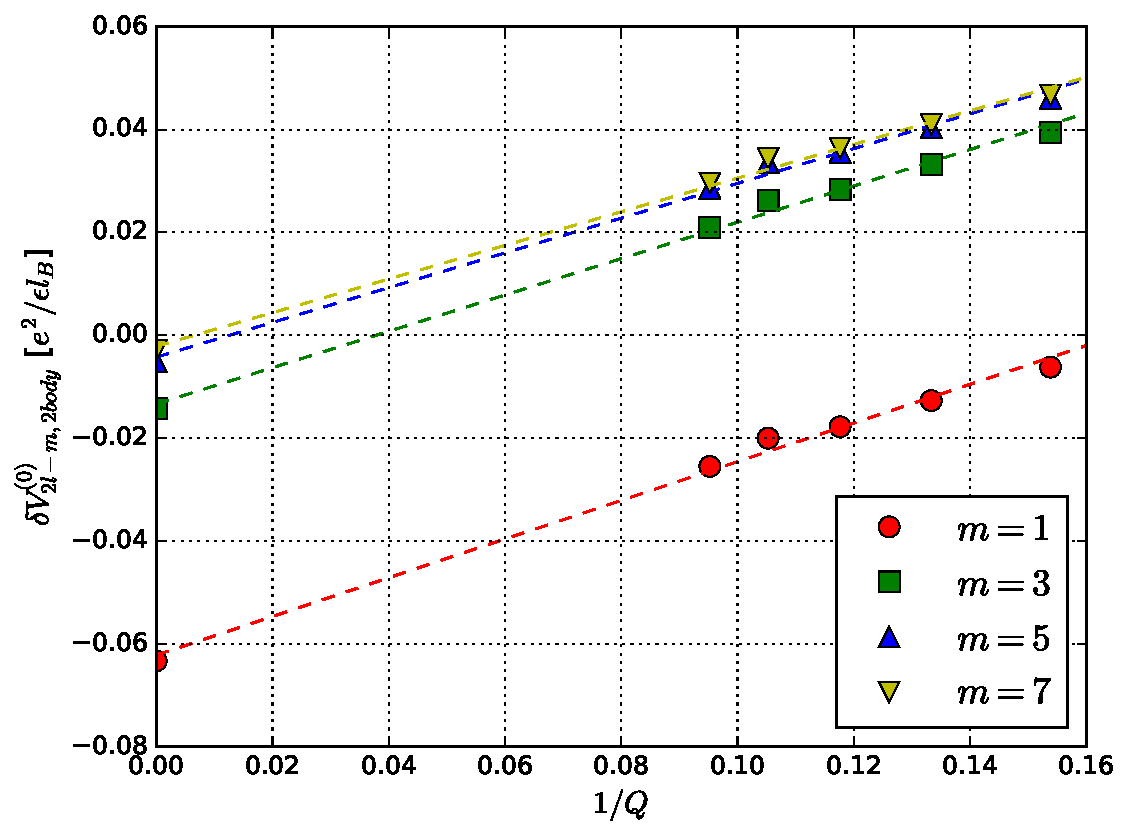
\includegraphics[width=10cm, angle=0]{ThesisCSULBLatexTemplate/figures/delta_vs_1_over_q.pdf}
    \caption[The approximate two-body Haldane pseudopotential corrections.]{The approximate two-body Haldane pseudopotential corrections. The dotted lines represent the fitted equations for the lowest Landau level PP corrections, $\delta V^{(0)}_{2l-m,2body}$, at each of the first four odd values of the relative angular momentum $m$ as a function of the inverse of the magnetic monopole strength $1/Q$.}
    \label{fig:delta_vs_1_over_q} 
    \end{center}
    \end{figure}
    
    \subsection{Effective Real Space Potential} \label{ssec:realSpaceEffPot}
    
    The user-defined functions written in the programming language \texttt{Python 3.8} for the following calculations can be found in Appendix \hyperref[appendixA]{A}. They use the libraries \texttt{pandas}, \texttt{NumPy}, \texttt{SciPy}, and \texttt{SymPy} \cite{pandas,numpy,scipy,sympy}. 
    
    In Sec. \ref{sec:haldPseud}, we discussed the Park potential (Eq. \ref{parkPot}), which is an effective interaction in the lowest LL that produced the same PPs as the Coulomb interaction in the first-excited LL. We need a real space potential to calculate LLM-incorporated interactions in the MC code. Many real space interactions can produce the same PPs, and Lee $\textit{et al.}$ used the following form (in units of $e^{2}/\epsilon l_B$) which they found more convenient:
    \begin{equation} \label{leePot}
    V_{eff}(r)=\left(\sum_{j} c_{j} r^{2 j} e^{-r^{2}}+\frac{(2 n+1)^{-5 / 2}}{r}\right)\left[\frac{e^{2}}{\epsilon l_B}\right],
    \end{equation}
    where the parameters $c_j$ are produced by fitting the first five to six significant PPs exactly via the method described below \cite{lee}. As a reminder, the significant PPs are those at the lowest odd relative angular momentum values $m$ (see Sec.~\ref{sec:haldPseud}). The Lee potential required fitting $c_j$ for polynomial degrees higher than 2 which, when we adapted it to a continuous general formula/number of parameters as a function of the LLM parameter $\kappa$ and magnetic monopole strength $Q$ (see Sec.~\ref{ssec:apprEffPotPar}), ended up creating local minima that the Metropolis-Hastings algorithm got stuck in to produce energies with errors on the order of up to $10^6\%$ against the benchmarks produced by exact diagonalization (see Sec.~\ref{sec:enGaps}). We tried many combinations of elementary functions and numbers of parameters, but eventually settled on the following modified Park potential since it produced the most accurate energy gaps after being run through the the MC code in the LLL for our benchmarks at $\nu=1/3$, $6\leq N\leq10$, and $\kappa\in\{0.0,0.1,0.2\}$:
    \begin{equation} \label{modPark}
    V_{eff}(r)=\left(\frac{1}{r}+b_1e^{-\beta_1r}+b_2r^2e^{-\beta_2r}\right)\left[\frac{e^2}{\epsilon l_B}\right],
    \end{equation}
    where the distance $r$ is measured in units of magnetic length $l_B$. The degree of $r$ in the power of the exponential function was reduced, compared to the Park potential, in an attempt to push the effects of LLM towards larger $r$ values, which ended up being where the MC code was most sampling from (see Sec.~\ref{ssec:sourcErr} for more details on this). 
    
    We can map our effective potential to a LLM-incorporated PP via the following adaptation of the Wooten formula (Eq. \ref{wootPp}) to the LLL: 
    \begin{equation} \label{wootPpN0}
    V_{Q,Q}(L)=\frac{(-1)^{2Q+L}(2Q+1)^2}{\sqrt{Q}}\sum_{k=0}^{2Q}V_k
    \begin{Bmatrix}
    L&Q&Q\\k&Q&Q
    \end{Bmatrix}
    \begin{pmatrix}Q&k&Q\\
    -Q&0&Q
    \end{pmatrix}^2,
    \end{equation}
    where 
    \begin{equation} \label{wootPpVkN0}
    V_k=\frac{2k+1}{2}\int_{-1}^1V_{eff}(\sqrt{2(1-x)})P_k(x)dx.
    \end{equation}
    Once we have perturbatively added our LLM PP corrections to the bare Coulomb potential via Eq. \ref{potLlm}, we can use a modified Powell method (via the \texttt{root} method of the \texttt{scipy.optimize} library) to solve for the parameters $\{b_i,\beta_i\}$ that fit the modified Park potential exactly to the LLM-incorporated PPs at the first four odd $m$ values when mapped to the spherical geometry by the Wooten formula \cite{scipy}. 
    
    We now have a systematic method for fitting PP corrections, incorporating them in the spherical geometry, and fitting to them a real space potential that can be used in the MC code. The code used to generate these real space potentials (which can be found in Appendix \hyperref[appendixA]{A}) is contained in a \texttt{Jupyter Notebook} which was written with the intention of making changes for other material effects straightforward \cite{ipython}. Calculating a new real space potential for each system of interest, based on the LLM parameter $\kappa$ and number of electrons via the magnetic monopole strength $Q$ (see Sec.~\ref{ssec:apprEffPotPar}), required a lot of time from both the computer as well as the user. We noticed the process would be significantly more efficient if the real space potential were calculated directly in the MC code for each system via an equation for each fitting parameter, which we will discuss in the next section.
    
    \subsection{Approximating the Effective Potential Parameters} \label{ssec:apprEffPotPar}
    
    In the last section, we developed a framework for calculating the parameters that map the modified Park potential (Eq.~\ref{modPark}) to LLM-incorporated PPs in the spherical geometry. Since generating these parameters for each value of the LLM parameter $\kappa$ and magnetic monopole strength $Q$ is costly to both the computer's and user's time, we can approximately fit the parameters to polynomial functions of $\kappa$ and/or $Q$ and plug these functions directly into the MC code so there is no need to recalculate the parameters before each run. We generated data for $\kappa\in$ \{0.0, 0.1, 0.2, 0.5, 0.8, 0.9, 2.2\} and $Q\in$ \{4.5, 6.0, 7.5, 9.0, 10.5, 12.0, 13.5, 15.0, 18.0, 22.5, 28.5, 36.0, 43.5, 58.5, 73.5\}. From the total flux on the sphere for Laughlin states in the LLL at filling factor $\nu=1/3$, $2l=3(N-1)$, we have $Q=3/2(N-1)$. The chosen $Q$ values then correspond to the system sizes $N\in$ \{4, 5, 6, 7, 8, 9, 10, 11, 13, 16, 20, 25, 30, 40, 50\}. We chose $Q$ values that approach the thermodynamic limit slowly from the smaller values we want to benchmark against exact diagonalization, and we chose $\kappa$ values that would allow us to observe changes from the bare Coulomb potential to the different experimental graphene environments (e.g. substrates) discussed in Sec. \ref{ssec:landLevMix}. 
    
    Upon analyzing the data, we noticed that the parameters (from Eq.~\ref{modPark}) qualitatively followed relations of the form $b_i(Q,\kappa)=(c_1Q^{c_2}+c_3)\kappa$ and $\beta_i(Q)=c_1Q^{c_2}+c_3$, where $\{c_i\}$ are fitting parameters. The functions we obtained are as follows:
    \begin{eqnarray} \label{eqn:paramEq}
        b_1(Q,\kappa)&=&(-1.146076\;Q^{0.452216}-0.276487)\kappa \\ \label{eq:b2}
        b_2(Q,\kappa)&=&(0.000185\;Q^{2.274277}+0.484263)\kappa \\ \label{eq:beta1}
        \beta_1(Q)&=&0.906035\;Q^{0.537208}+1.811340 \\
        \beta_2(Q)&=&0.034071\;Q^{1.150906}+1.122173. \label{eqn:lastPar}
    \end{eqnarray} 
    We can see the fits of these functions against the data for chosen values of $\kappa$ at fixed $Q$ and vice versa in Figs. \ref{fig:b12_vs_q_k} and \ref{fig:beta12_vs_q_k} (similar behavior was observed when other $\kappa$ and $Q$ values were chosen). Our modified Park potential was originally expressed in terms of its fitting parameters, $V_{eff}(r,b_1,b_2,\beta_1,\beta_2)$, but it can now be plugged into the MC code directly as a function of the LLM parameter and magnetic monopole strength for each system of interest, giving us $V_{eff}(r,\kappa,Q)$. This means that any system inputted into the MC code will now automatically generate its corresponding LLM-incorporated effective real space potential. This fitting will introduce some error, but we are only concerned with the error in the PPs. We will discuss this further in the next section.
    
    \begin{figure}[h]
    \begin{center}
    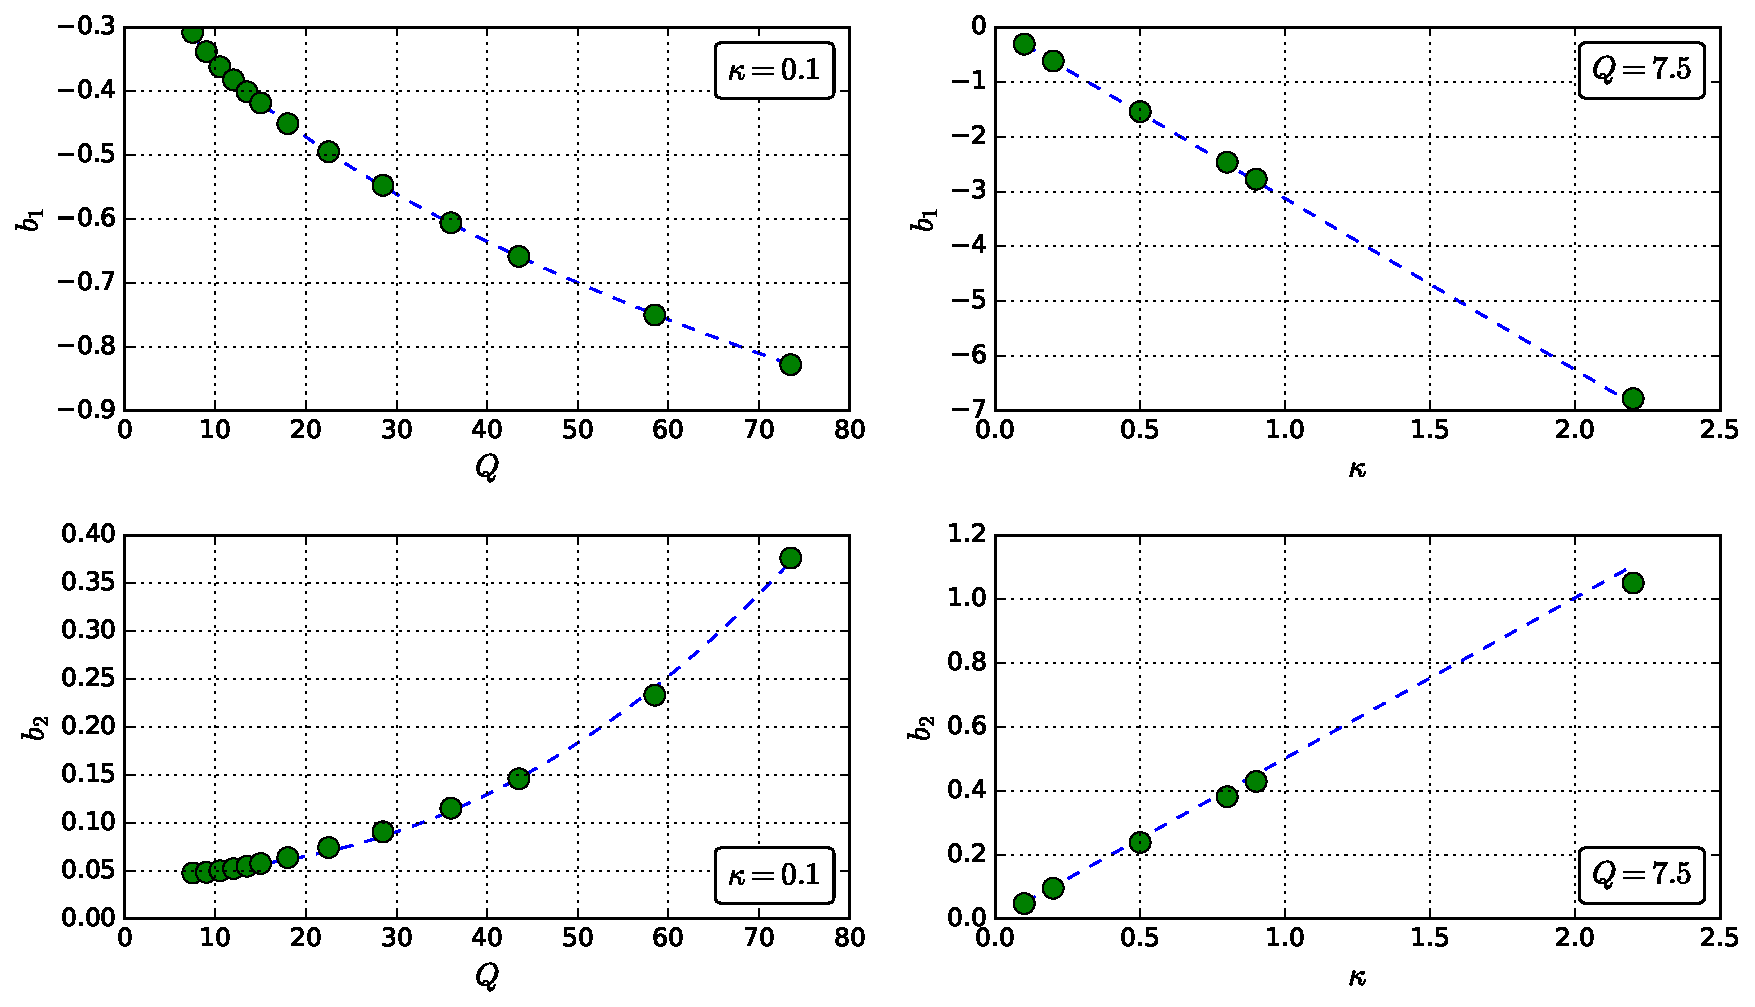
\includegraphics[width=10cm, angle=0,scale=1.5]{ThesisCSULBLatexTemplate/figures/b12_vs_q_k.pdf}
    \caption[The approximate effective real space potential parameters $b_i$.]{The approximate effective real space potential parameters $b_i$. The parameter functions $b_i$ (Eqs.~\ref{eqn:paramEq} and~\ref{eq:b2}) for the lowest Landau level with filling factor $\nu=1/3$ are plotted either at fixed LLM parameter $\kappa=0.1$ or fixed magnetic monopole strength $Q=7.5$.}
    \label{fig:b12_vs_q_k} 
    \end{center}
    \end{figure}
    
    \begin{figure}[h]
    \begin{center}
    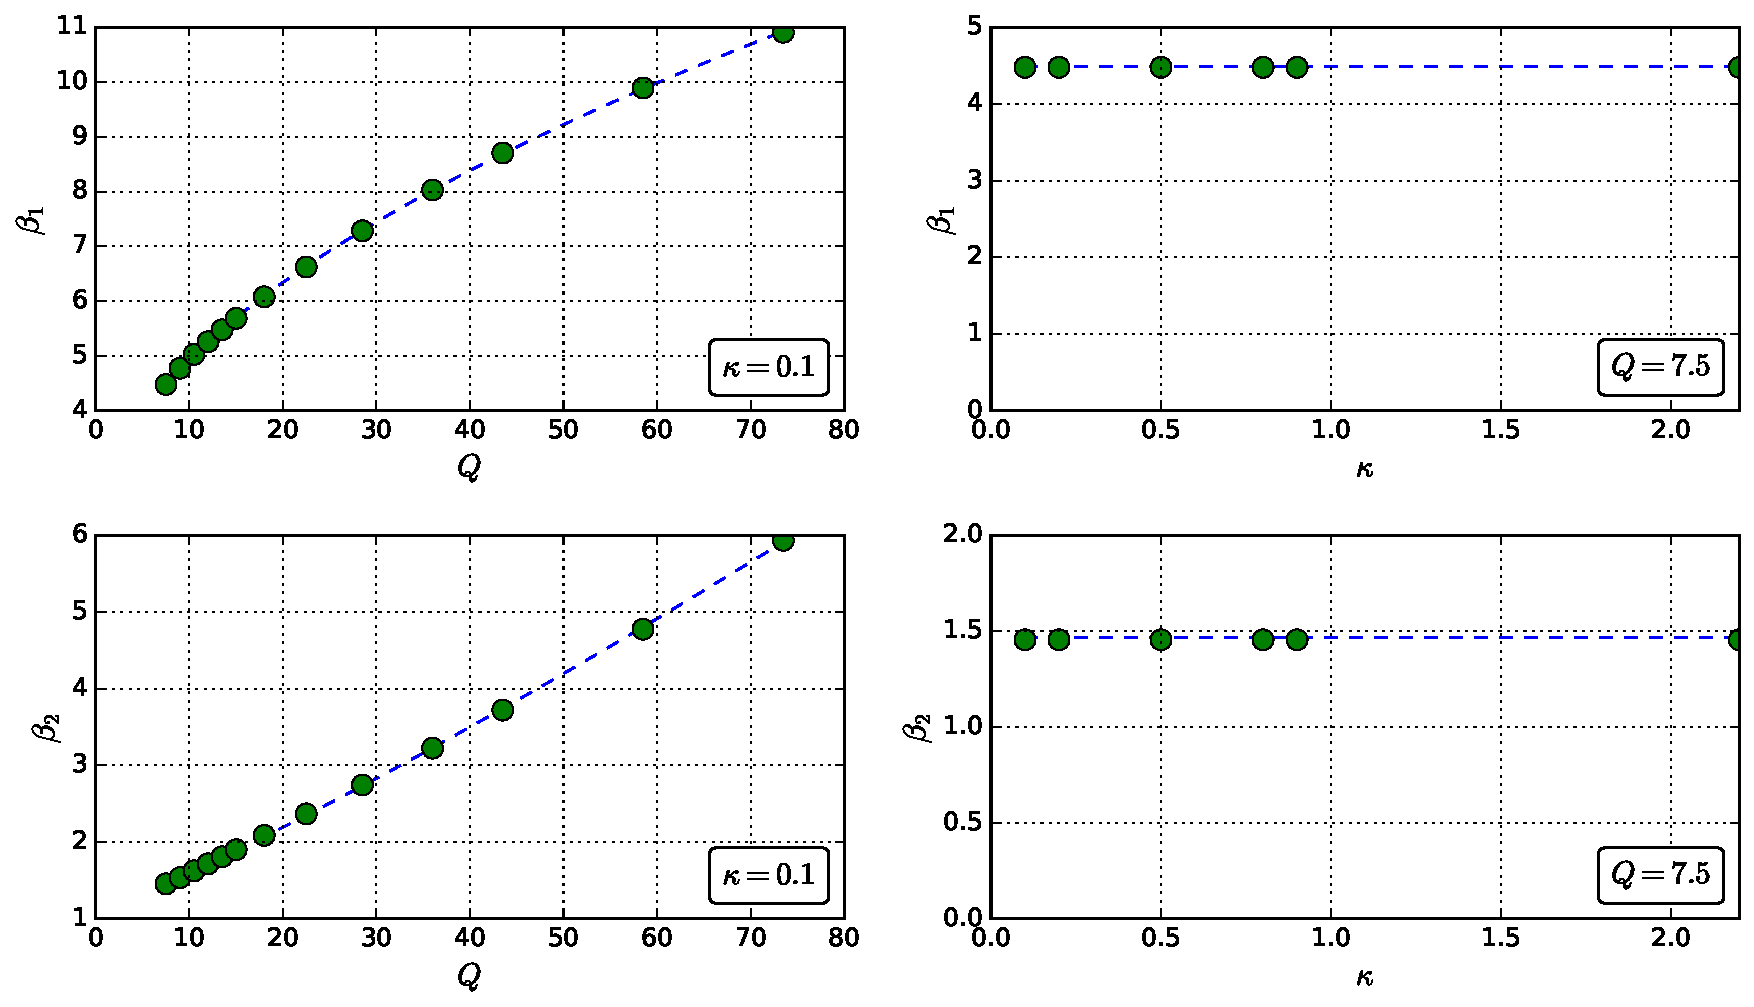
\includegraphics[width=10cm, angle=0,scale=1.5]{ThesisCSULBLatexTemplate/figures/beta12_vs_q_k.pdf}
    \caption[The approximate effective real space potential parameters $\beta_i$.]{The approximate effective real space potential parameters $\beta_i$. The parameter functions $\beta_i$ (Eqs.~\ref{eq:beta1} and~\ref{eqn:lastPar}) for the lowest Landau level with filling factor $\nu=1/3$ are plotted either at fixed LLM parameter $\kappa=0.1$ or fixed magnetic monopole strength $Q=7.5$.}
    \label{fig:beta12_vs_q_k} 
    \end{center}
    \end{figure}
    
    \subsection{The Approximated Effective Real Space Potential} \label{ssec:apprEffPot}
    
    We can remember from Sec. \ref{ssec:landLevMix} that we are incorporating LLM via Eq. \ref{potLlm}, or in other words perturbatively adding the fitted LLM PP corrections to the PPs in the spherical geometry that the bare Coulomb potential was mapped to by the Wooten formula (Eq.~\ref{wootPpN0}). We can observe how LLM changes the bare Coulomb PPs in the spherical geometry as a function of the relative angular momentum $m$ in Fig. \ref{fig:coul_llm_vs_m}. For $Q=7.5$ in the LLL, LLM shifts the corrected PPs vertically downwards from the bare Coulomb PPs for $m=1$, and then upwards for $m>1$. We can then think of LLM as "flattening" the bare Coulomb PPs, or decreasing the magnitude of their mean slope as a function of increasing $m$. We will see shortly that this flattening of the PPs carries over into the effective potential in real space as well. We can see in the figure that the PP flattening increases with increasing $\kappa$. Therefore, we should see the gaps between energies decrease with increasing $\kappa$, which is the trend produced by the exact diagonalization benchmarks (see Sec.~\ref{ssec:benchmRes}). We should mention that these perturbative corrections, although we use them for $\kappa$ up to 2.2 to simulate experimental graphene environments, are designed for the $\kappa\ll1$ limit - further study still needs to be done to determine the accuracy of this perturbative model in the $\kappa$ order unity limit. 
    
    \begin{figure}[H]
    \begin{center}
    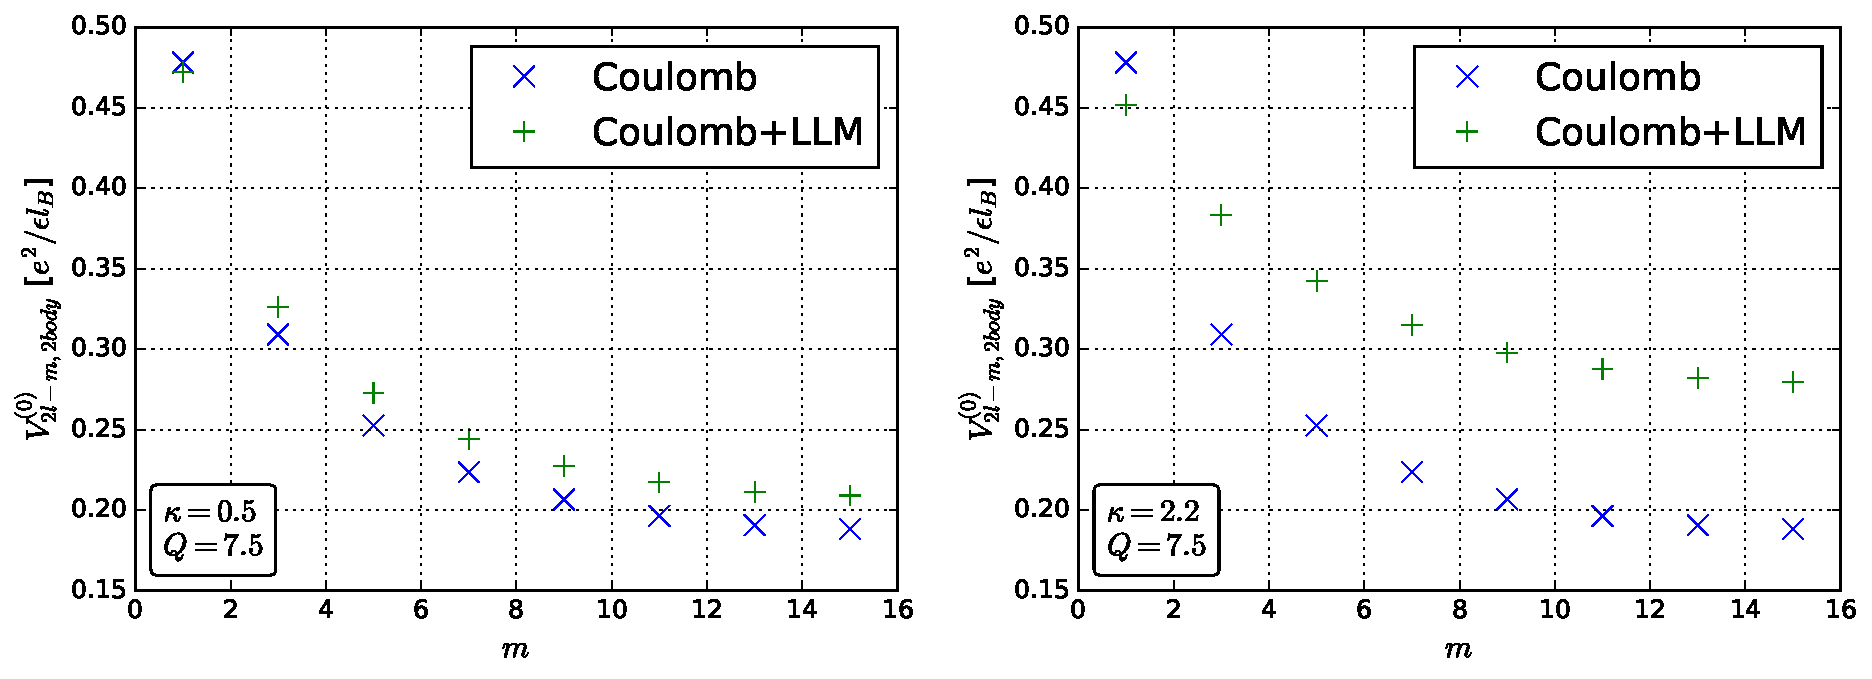
\includegraphics[width=10cm, angle=0,scale=1.5]{ThesisCSULBLatexTemplate/figures/coul_llm_vs_m.pdf}
    \caption[The Landau level mixing-incorporated Haldane pseudopotentials.]{The Landau level mixing-incorporated Haldane pseudopotentials. We perturbatively added (Eq.~\ref{potLlm}) our fitted LLM PP corrections to the PPs the bare Coulomb potential was mapped to in the spherical geometry by the Wooten formula (Eq.~\ref{wootPpN0}) in the LLL for magnetic monopole strength $Q=7.5$ and LLM parameter $\kappa\in\{0.5,2.2\}$. We plot the bare Coulomb PPs and the LLM corrected PPs as a function of the relative angular momentum $m$.}
    \label{fig:coul_llm_vs_m} 
    \end{center}
    \end{figure}

    \vspace{24pt} % keep uniform double space below caption
    
    Once we have incorporated LLM into our PPs in the spherical geometry, we can fit to them an effective real space potential at the first four odd $m$ values exactly via the Wooten formula (Eq.~\ref{wootPpN0}), which can be seen in the plot in Fig. \ref{fig:vEff_vs_m}. As expected when fitting only the first four odd $m$ corrected PPs exactly, the PPs produced by the effective real space potential start to slowly deviate from the corrected PPs for larger $m$ values, and this trend is exaggerated as $\kappa$ increases. As mentioned in Sec. \ref{sec:haldPseud}, we are most interested in the first significant PP values since that is where the Coulomb interaction, the origin of LLM, is the strongest. Larger $m$ PPs affect the overall physics less since they correspond with long distance behavior and, in any case, the differences are rather small quantitatively.
    
    \begin{figure}[H]
    \begin{center}
    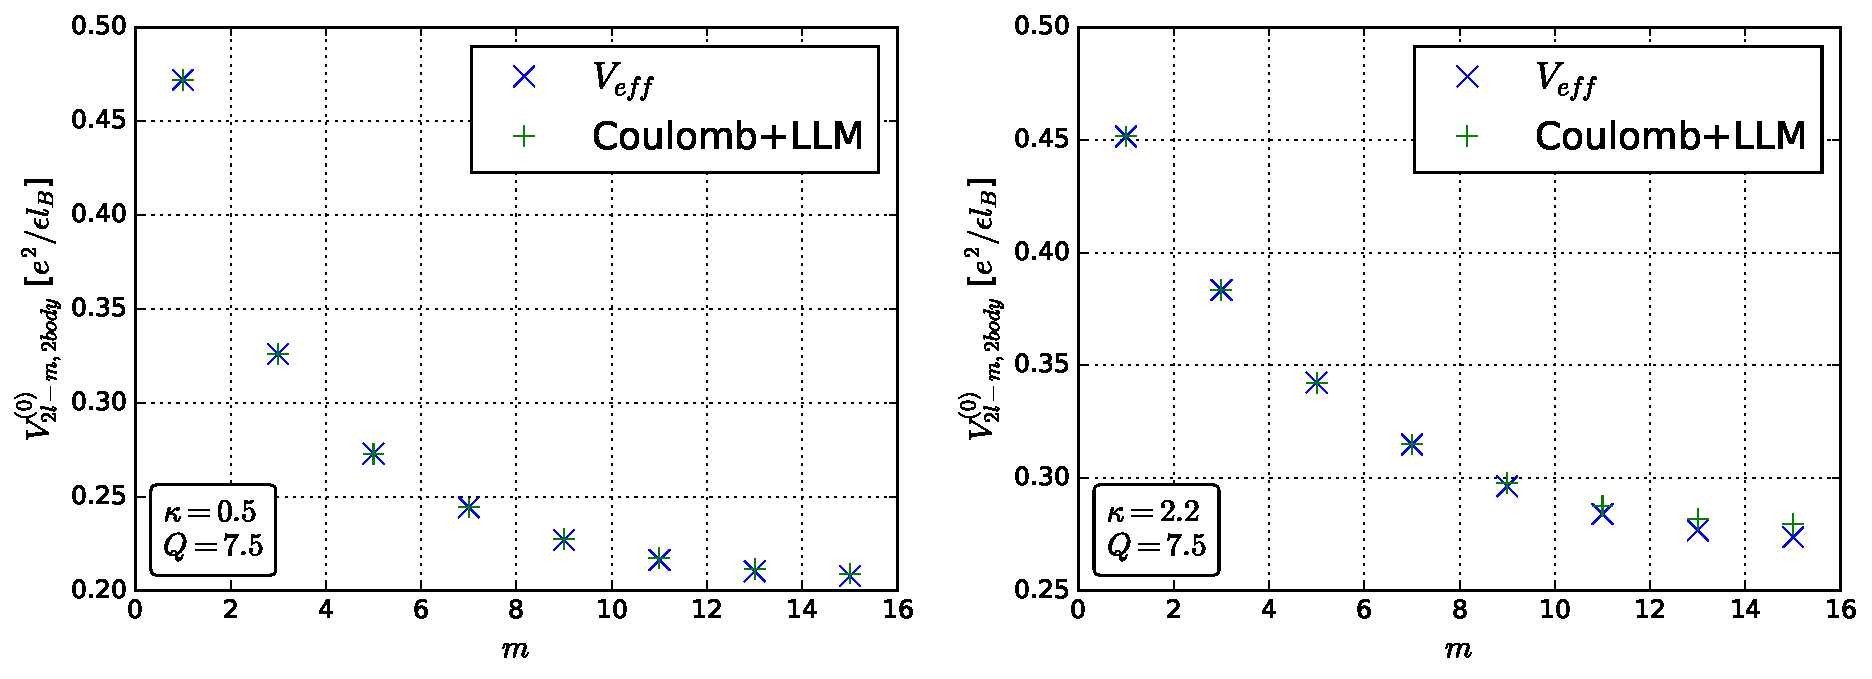
\includegraphics[width=10cm, angle=0,scale=1.5]{ThesisCSULBLatexTemplate/figures/vEff_vs_m.pdf}
    \caption[The fit of the PPs produced by the effective real space potential to the LLM-incorporated PPs.]{The fit of the PPs produced by the effective real space potential to the LLM-incorporated PPs. The two-body, effective real space potential $V_{eff}$ (Eq.~\ref{modPark}) is mapped to PPs on the Haldane sphere via the Wooten formula (Eq.~\ref{wootPpN0}) and then fit to LLM-incorporated PPs in the LLL exactly for the first four odd values of the relative angular momentum $m$ with magnetic monopole strength $Q=7.5$ and LLM parameters $\kappa\in\{0.5,2.2\}$. The PPs are plotted as a function of momentum $m$.}
    \label{fig:vEff_vs_m} 
    \end{center}
    \end{figure}
    
    Fitting the PPs produced by the modified Park potential exactly to the first four odd $m$ LLM-incorporated PPs before each run of the MC code for each combination of $\kappa$ and $Q$ took a long time for both the computer and the user. Before our method, this had to be done to solve for the parameters of the effective potential that needed to be manually plugged into the MC code for each unique system. In the previous section, we developed functions for each parameter (Eqs.~\ref{eqn:paramEq} -~\ref{eqn:lastPar}) which are now used to calculate directly in the MC code the modified Park potenial parameters that approximately fit the first four odd $m$ LLM-incorporated PPs in the LLL when mapped to PPs in the spherical geometry by the Wooten formula. We can observe the error introduced into the LLM-incorporated PP calculations due to using the approximated modified Park potential fitting parameters in Fig. \ref{fig:pp_err_vs_m}. The \% error was calculated by
    \begin{equation}\label{eq:perc_err}
    \frac{|V_{eff}-(\text{Coulomb}+\text{LLM})|}{\text{Coulomb}+\text{LLM}}*100\%,
    \end{equation}
    where $V_{eff}$ are the PPs produced by the approximated modified Park potential and $\text{Coulomb}+\text{LLM}$ are the PPs produced by perturbatively adding the fitted LLM PP corrections to the PPs produced by the bare Coulomb potential via Eq.~\ref{potLlm}. Even for our largest LLM parameter, $\kappa=2.2$, the PPs produced by the approximated modified Park potential at the first four odd $m$ values with $Q=7.5$ are still accurate to less than 1\% error. In our simulations, the \% error at the first four $m$ values was found to decrease with increasing $Q$. We can see in the figure, however, that the \% error increases for larger $m$ values. We believe this has less bearing on the physics because the PPs at large $m$ values are very small, and therefore the \% errors can increase without significantly changing the physics.
    
    \begin{figure}[h]
    \begin{center}
    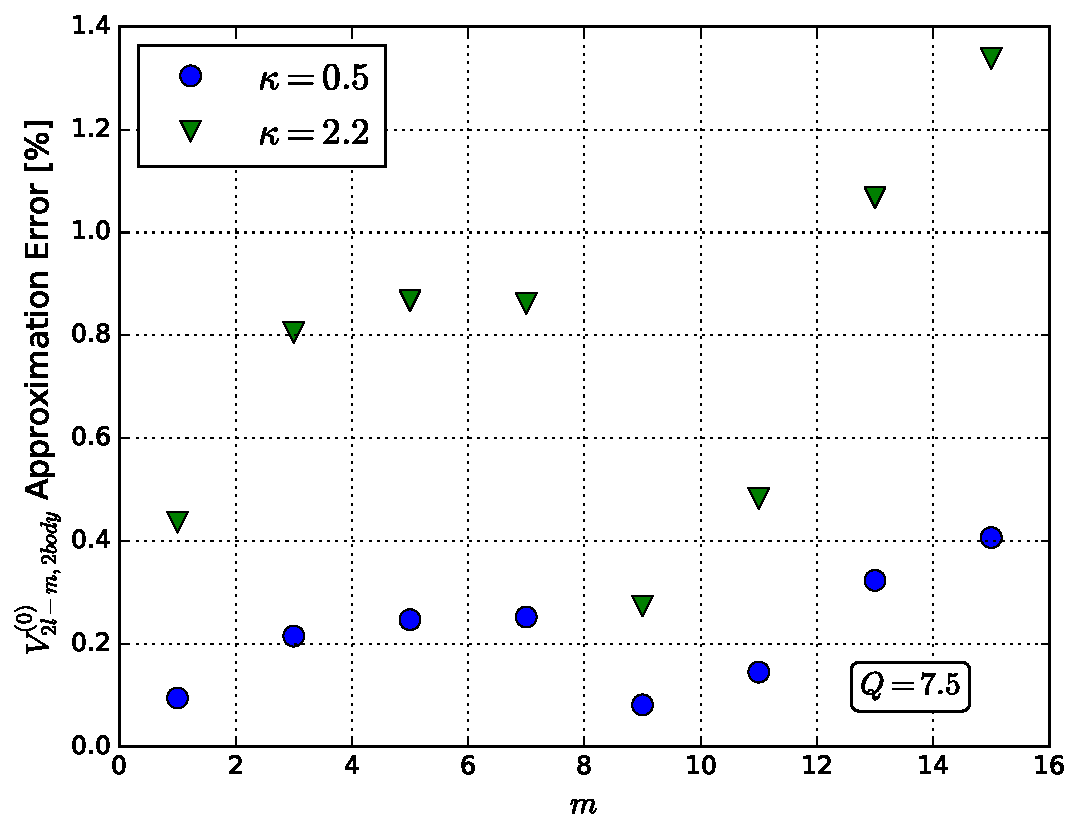
\includegraphics[width=10cm, angle=0]{ThesisCSULBLatexTemplate/figures/pp_err_vs_m.pdf}
    \caption[LLM-incorporated Haldane pseudopotential aproximation error.]{LLM-incorporated Haldane pseudopotential aproximation error. The LLL two-body PPs in the spherical geometry, $V^{(0)}_{2l-m,2body}$, were approximated using the parameter functions (Eqs.~\ref{eqn:paramEq} -~\ref{eqn:lastPar}). We plot the \% error due to this approximation as a function of the relative angular momentum $m$ with magnetic monopole strength $Q=7.5$ and LLM parameter $\kappa\in\{0.5,2.2\}$. The parameter functions were fit approximately to data which was fit exactly to the LLM-incorporated PPs at the first four odd $m$ values.}
    \label{fig:pp_err_vs_m} 
    \end{center}
    \end{figure}
    
    We have now developed an accurate and significantly less computationally complex method of calculating a realistic effect-incorporated effective real space potential for MC simulations of FQH energies. We want to stress that this framework was structured so that it can easily be adapted to incorporating other realistic effects besides LLM (e.g. disorder) in other materials besides graphene by making minimal changes to an existing \texttt{Jupyter Notebook} given some PP correction data.
    
    We can see what the modified Park potential looks like in real space as a function of the chord distance between electrons on the Haldane sphere $r$ in Fig. \ref{fig:vEff_vs_r}. For small distances at $Q=7.5$, the effective potential dips below the Coulomb potential before rising above it and then quickly converging to it at farther distances. This dip becomes more pronounced as $\kappa$ increases, which is easier to see in the plot of the difference between the approximated modified Park potential and the bare Coulomb potential, $V_{eff}-V_{Coul}$, for different values of $\kappa$ in Fig. \ref{fig:vEff_minus_vCoul_vs_r}. One of the reasons we chose the modified Park potential was because it was well behaved in real space, or has no local minima for the values in the figure (e.g. compared to the Lee potential - see Sec.~\ref{ssec:realSpaceEffPot} for more details). We would like to direct the reader to Appendix \hyperref[appendixB]{B} for a discussion of mathematically interesting behaviors of the modified Park potential in real space, including why the differences seem to intersect at one point as well as the behavior of the difference as a function of $Q$. In the next section, we discuss changes made to the MC code to continue to make the process of calculating the FQH energy gaps even more efficient.
    
    \begin{figure}[H]
    \begin{center}
    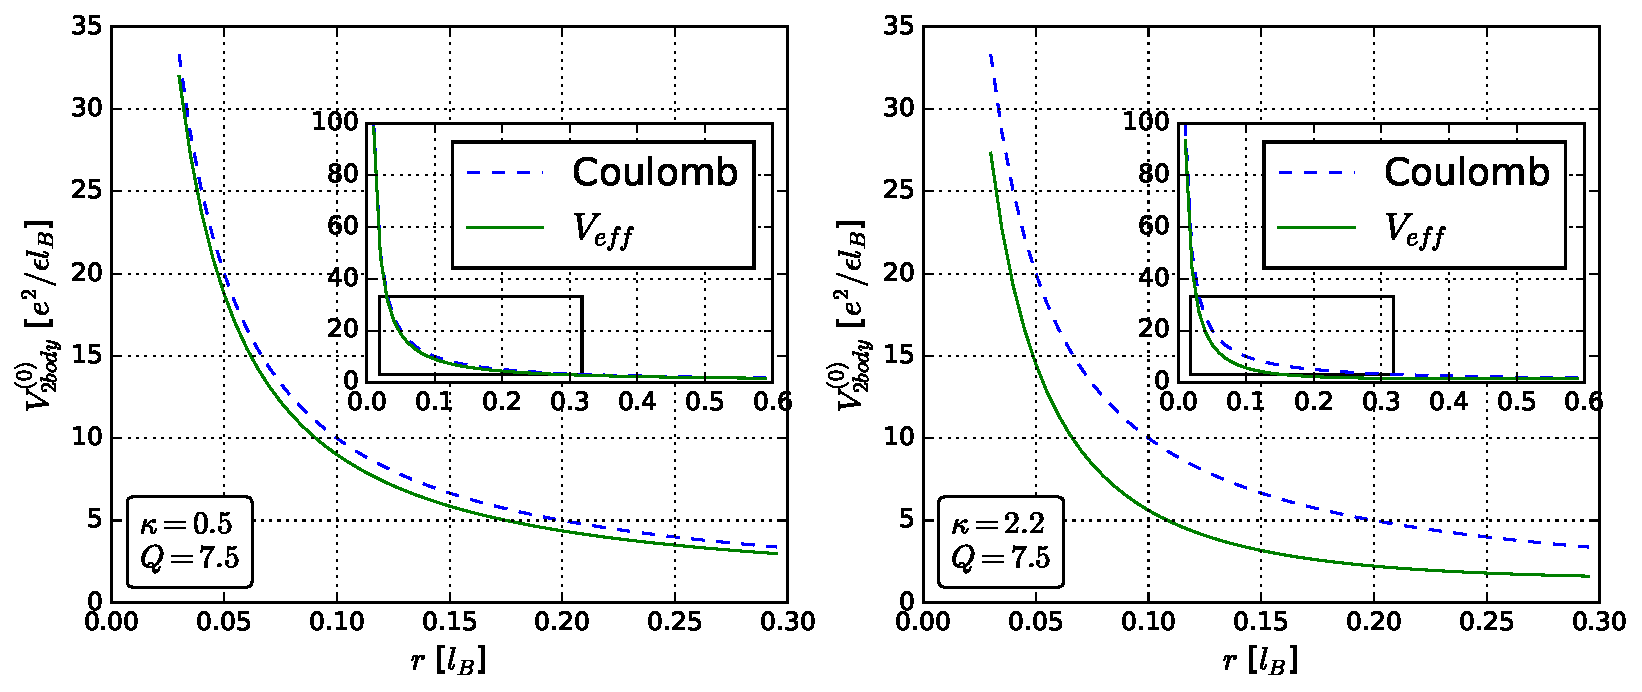
\includegraphics[width=10cm, angle=0,scale=1.5]{ThesisCSULBLatexTemplate/figures/vEff_vs_r.pdf}
    \caption[The modified Park potential in real space.]{The modified Park potential in real space. The modified Park potential and Coulomb potential are plotted in real space as a function of the chord distance between electrons $r$ for $0<r\leq0.30$, magnetic monopole strength $Q=7.5$, and LLM parameter $\kappa\in\{0.5,2.2\}$. The inset shows the behavior of the potentials for $0<r\leq0.60$.}
    \label{fig:vEff_vs_r} 
    \end{center}
    \end{figure}
    
    \begin{figure}[H]
    \begin{center}
    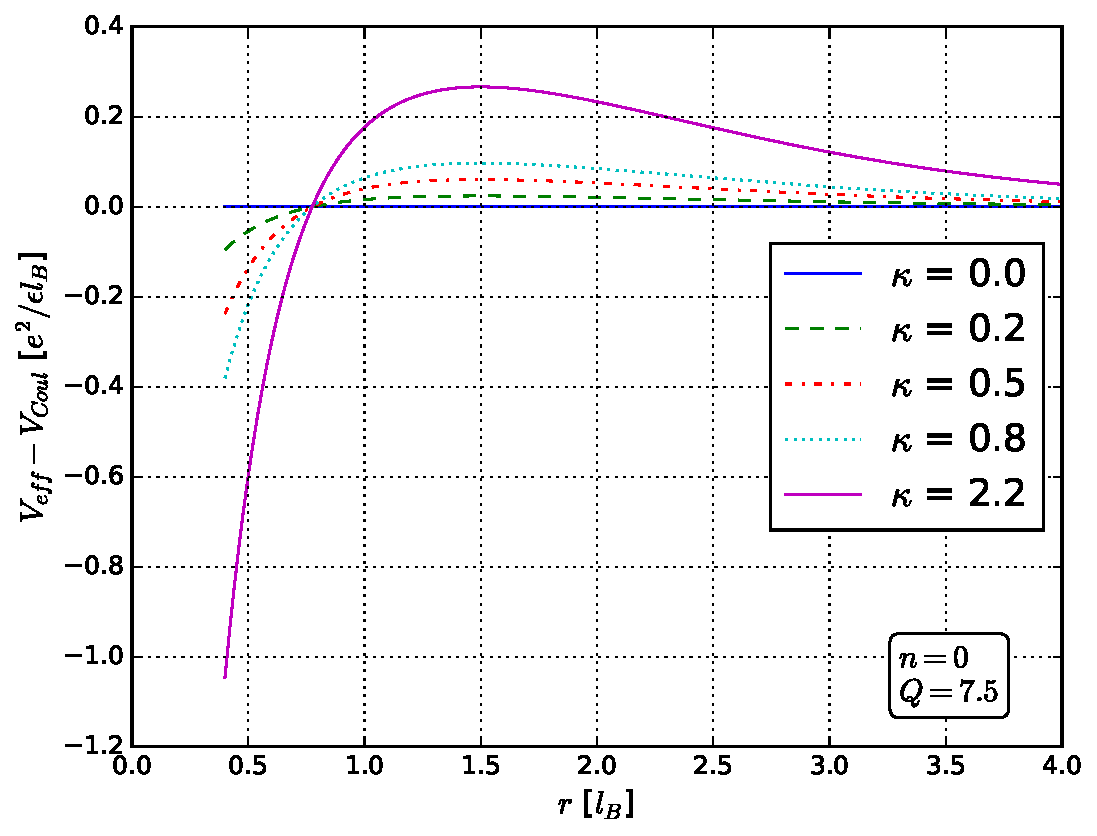
\includegraphics[width=10cm, angle=0]{ThesisCSULBLatexTemplate/figures/vEff_minus_vCoul_vs_r.pdf}
    \caption[The difference between the modified Park potential and the Coulomb potential.]{The difference between the modified Park potential and the Coulomb potential. The difference $V_{eff}-V_{Coul}$ is plotted for $0<r\leq4.0$ with magnetic monopole strength $Q=7.5$ and LLM parameter $\kappa\in\{0.0,0.2,0.5,0.8,2.2\}$.}
    \label{fig:vEff_minus_vCoul_vs_r} 
    \end{center}
    \end{figure}
    
    \subsection{The Monte Carlo Code and the Composite Fermion-Exciton Dispersion} \label{ssec:compFermExcDisp}
    
    In this section, we discuss some of the intermediate changes made to the MC code in the course of calculating an accurate exciton dispersion for the bare Coulomb potential as a baseline before moving onto the LLM-incorporated effective real space potential. Before our method, the process of incorporating realistic effects into MC simulations of the FQHE was quite complex. Obtaining all the PP corrections for a system of interest is nontrivial. Using Wooten's formula to fit an effective real space potential to the realistic effect-incorporated PPs in the spherical geometry for each system of interest takes a long time for both the computer and the user. Incorporating these changes into the MC code also took a long time because the values that need to be changed for each system were scattered among thousands of lines of code. With our \texttt{Jupyter Notebook}, all you need to plug in is a handful of PP corrections, and then as output you receive the parameter equations (Eqs.~\ref{eqn:paramEq} -~\ref{eqn:lastPar}) which can be entered into the MC code so that it automatically generates the effective real space potential as a function of the realistic effect parameter $\kappa$ and magnetic monopole strength $Q$. In this thesis, we apply our method to the specific example of LLM in graphene, where we focus on two-body interactions in the LLL, but the method was designed to be more generally applicable. 
    
    The matter still remained, however, of the inefficiency of changing all the corresponding variables for each run. These variables (the number of iterations \textt{ITER}, the $\Lambda$ level filling factor \texttt{NLL}, the realistic effect parameter \texttt{vEffKappa}, the number of electrons/CFs \texttt{N}, and a boolean value representing whether you want to calculate all the energy gaps or just the transport gap \texttt{transpGapQ}) are now inputted into a script that runs the code in parallel across a desired number of cores of the California State University Long Beach central High Performance Computing (HPC) cluster. All the relevant data is now also outputted into a neatly organized CSV file. All systems of interest (i.e. electron filling factors, realistic effect parameters, system sizes, etc.) can be run by a single script, on the order of tens of minutes for the benchmark calculations we perform in the next chapter, the results of which can be imported into the built-in analysis section of the \texttt{Jupyter Notebook} for quick visualization of the data.
    
    Once we could quickly have our MC code generate a LLM-incorporated effective real space potential, we set out to calculate the low energy (see Sec.~\ref{sec:compFerm}) CF-exciton dispersion $\Delta$ of realistic graphene systems in the LLL. However, after plugging the parameter equations and \texttt{RANGE} equation (which determines the acceptance ratio of the Metropolis-Hastings algorithm, please see Appendix \hyperref[appendixC]{C} for more details) into the MC code, the exciton dispersion was observed to diverge for large wave vectors $kl=L/\sqrt{Q}$ (see Fig. \ref{fig:exc_disp_samples}). The MC code was originally designed using the ground state (corresponding to total angular momentum $L_0=0$) wavefunction to calculate the probability weight function for acceptance sampling. In Sec. \ref{ssec:montCarlInt}, we mentioned that to efficiently do MC, one chooses configurations via importance sampling. This is done typically by using the ground state ($L_0=0$) wavefunction to calculate the probability of being in the trial state vs. the previous state. In principle, any function can be chosen, including a constant, for importance sampling. It makes the most sense to choose the wavefunction for the current state $L_i$, but that increases the number of operations by a factor of $N$. We found that using just the wavefunction of the lowest energy state at the maximum total angular momentum ($L_{max}=N$) produced an accurate exciton dispersion. Fig.~\ref{fig:exc_disp_samples} shows the dispersion $\Delta$ for the bare Coulomb potential as a function of the wave vector $kl$ produced by using the wavefunctions from the different states $L_{sample}$ for acceptance sampling in the LLL with $N=11$ electrons at filling factor $\nu=1/3$. The mean error of the energy gaps calculated using $L_{max}$ (vs. the values produced by $L_i$) for all $kl$ values is 2.0\%, with a maximum of 3.3\% and standard deviation of 0.94\%. Further study needs to be done to explore the cause of the divergence of the dispersion when using $L_0$, but we believe that the ground state wavefunction is too naive a guess for the more complicated, higher total angular momentum state wavefunctions, therefore requiring significantly more Metropolis-Hastings iterations for convergence of the energy gaps (see Sec.~\ref{ssec:compFerm}). We found that using $L_{max}$ allowed us to get an accurate exciton dispersion for the bare Coulomb potential for larger system sizes - we plot the dispersion for $N=20$ electrons in Fig.~\ref{fig:exc_disp_n_20}. Now that we can efficiently and accurately calculate the exciton dispersion for the bare Coulomb potential, we can benchmark the LLM-incorporated exciton dispersion against exact diagonalization in the next chapter.
    
    \begin{figure}[H]
    \begin{center}
    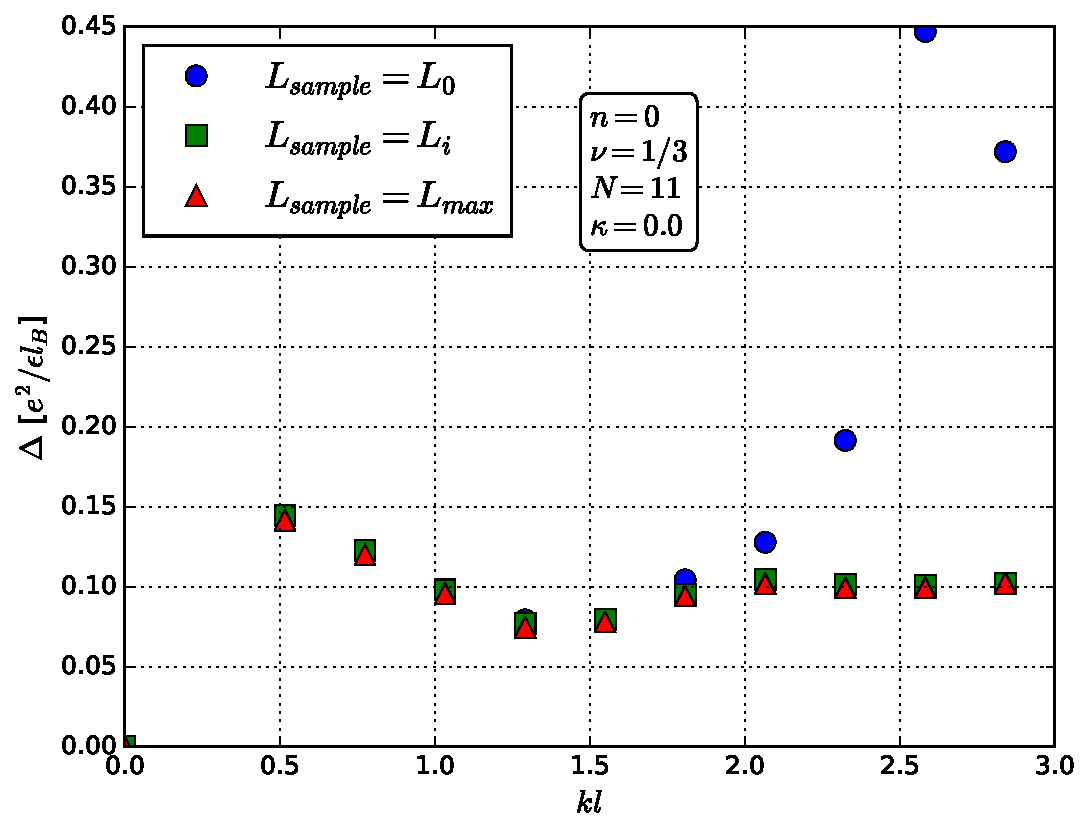
\includegraphics[width=10cm, angle=0]{ThesisCSULBLatexTemplate/figures/exc_disp_samples.pdf}
    \caption[The CF-exciton dispersion when using wavefunctions of different states for Metropolis-Hastings acceptance sampling.]{The CF-exciton dispersion when using wavefunctions of different states for Metropolis-Hastings acceptance sampling. We plot the exciton dispersion $\Delta$ for the bare Coulomb potential ($\kappa=0.0$) vs. the wave vector $kl$ in the LLL for $N=11$ electrons at filling factor $\nu=1/3$ produced by using three different types of total angular momentum state wavefunctions as the probability weight function for acceptance sampling in the Metropolis-Hastings algorithm: the ground state $L_0$, each individual state $L_i$, and the lowest energy state at maximum total angular momentum $L_{max}$. The dispersion for $L_0$ diverges at large wave vectors, while the dispersion for $L_{max}$ closely matches the most accurate dispersion calculated using each individual state $L_i$.}
    \label{fig:exc_disp_samples} 
    \end{center}
    \end{figure}

    \begin{figure}[p]
    \begin{center}
    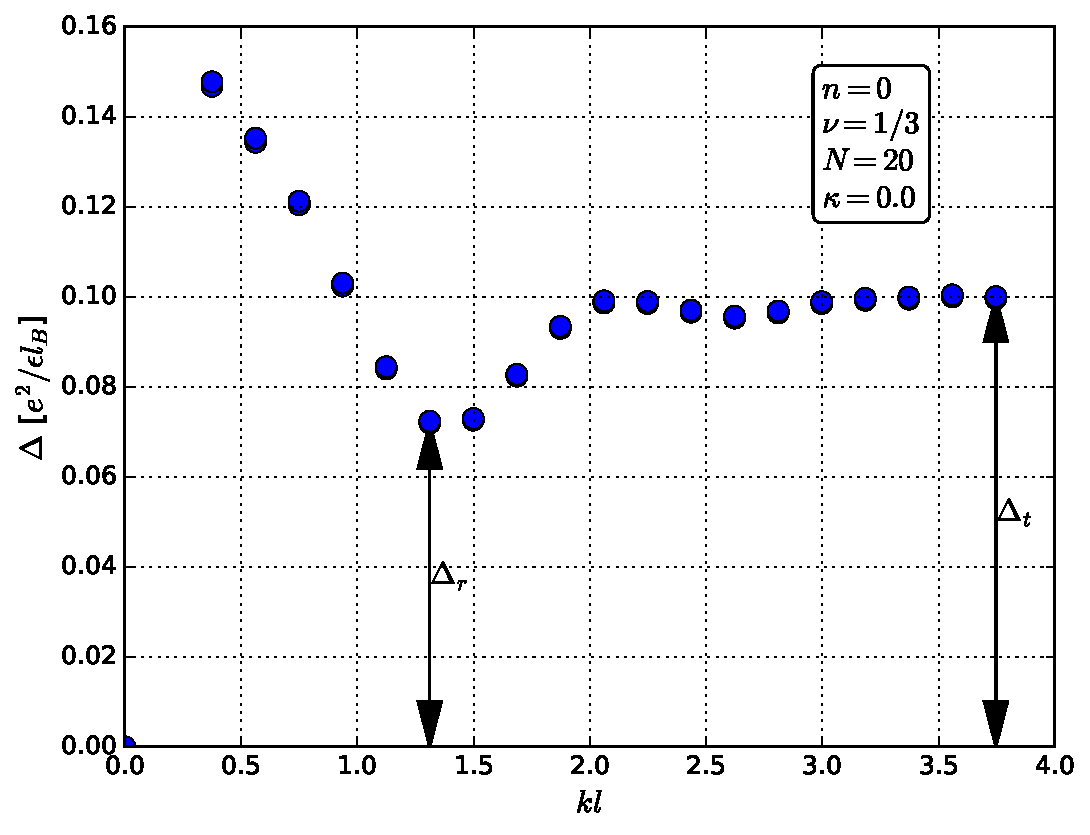
\includegraphics[width=10cm, angle=0]{ThesisCSULBLatexTemplate/figures/exc_disp_n_20.pdf}
    \caption[The CF-exciton dispersion for the bare Coulomb potential with $N=20$ electrons.]{The CF-exciton dispersion for the bare Coulomb potential with $N=20$ electrons. We plot the exciton dispersion $\Delta$ vs. the wave vector $kl$ for the bare Coulomb potential ($\kappa=0.0$) in the LLL ($n=0$) for $N=20$ electrons at filling factor $\nu=1/3$. The minimum (roton $\Delta_r$) and constant approached at large wave vectors for a far separated CF-quasiparticle and CF-quasihole pair (transport gap $\Delta_t$) are indicated. The probability weight function used for Metropolis-Hastings acceptance sampling was the wavefunction for the lowest energy state at maximum total angular momentum $L_{max}$.}
    \label{fig:exc_disp_n_20} 
    \end{center}
    \end{figure}

\singlespacing


\chapter{BENCHMARKS}\label{ch:3}
\doublespacing

In the previous chapter, we developed a systematic method for constructing effective real space potentials that incorporate realistic effects into Monte Carlo (MC) simulations of the fractional quantum Hall effect (FQHE). In this chapter, we apply our method to the effect of Landau level mixing (LLM) in the lowest Landau level (LLL) of graphene. We calculate the composite fermion (CF)-exciton dispersion via MC and benchmark the results against an exact calculation via exact diagonalization.

\section{Composite Fermion-Exciton Dispersion for Small Systems} \label{sec:enGaps}

    \subsection{Exact Diagonalization} \label{ssec:exDi}
    In order to benchmark the MC calculations, which are approximate by nature, we can calculate the exciton disperson exactly for small systems ($N\lesssim 10$).  Since this thesis focuses mostly on constructing real space potentials describing realistic effects for use in MC calculations, we will only briefly outline how the exact calculations are done. 
    
    The CF wavefunction for electron filling factor $\nu=1/3$ is equivalent to the Laughlin wavefunction. It turns out that this state can be written as an exact expansion of Slater determinants (basis states) by exactly diagonalizing the so-called ``hard core", or ``$V_1=\infty$", potential~\cite{haldane}. Practically, this means we set the ratio of $V_1/V_m\rightarrow\infty$ for all $m\neq 1$. This amounts to exactly diagonalizing the Hamiltonian in Eq.~\ref{HamPPexpand} with $V_m/V_1=0$ for all $m\neq 1$. In the spherical geometry, in which we work, this translates to setting $V_{Q,Q}(L)/V_{Q,Q}(2Q-1)=0$ for all $L\neq 2Q -1$. The Laughlin state $|\Psi_{1/3}(L=0)\rangle$ is the zero energy ground state of the aforementioned Hamiltonian. We can also find the low energy branch of excitations for calculating the exciton dispersion (see Sec.~\ref{sec:compFerm}) by diagonalizing the ``hard-core" potential $|\Psi_{1/3}(L)\rangle$. 
    
    Given the Haldane pseudopotentials (PPs) of a realistic FQH state (e.g. graphene on a substrate), we can insert Eq.~\ref{potLlm} into Eq.~\ref{HamPPexpand} to construct the Hamiltion as
    \begin{eqnarray}
    H_\mathrm{realistic} = \sum_m (V_m^{(0)} + \kappa \delta V_m^{(0)})\sum_{i<j} P_{ij}(m),
    \end{eqnarray}
    where the PPs are calculated using the single-particle basis states making up the Slater determinants. Now we can exactly calculate the exciton dispersion for $\nu=1/3$ by calculating the expectation value
    \begin{eqnarray}
    \frac{\langle \Psi_{1/3}(L)|H_\mathrm{realistic}|\Psi_{1/3}(L)\rangle}{\langle \Psi_{1/3}(L)|\Psi_{1/3}(L)\rangle}\;.
    \end{eqnarray}
    
    In the next section, we use these exact calculations to benchmark the MC exciton dispersion for $6\leq N\leq10$ electrons with LLM parameter $\kappa\in\{0.0,0.1,0.2\}$.

\iffalse    
    In this section, we will briefly sketch the method for which the CF ground state and low-energy excitation eigensystem can be obtained via exact diagonalization following from Appendix L of Ref. \cite{jain}.
    
    To diagonalize the Hamiltonian matrix, we must orthogonalize the CF basis functions of LLL projected wave functions via the Gram–Schmid procedure. We begin with the normalized states
    
    \begin{equation}\label{normStat}
    \left|\eta_{\alpha}\right\rangle \equiv \frac{\left|\Psi_{\alpha}\right\rangle}{\sqrt{\left\langle\Psi_{\alpha} \mid \Psi_{\alpha}\right\rangle}},
    \end{equation}
    
    with scalar products $\mathcal{O}_{\alpha \beta} \equiv\left\langle\eta_{\alpha} \mid \eta_{\beta}\right\rangle$. We can find the orthogonal basis states 
    
    \begin{equation}\label{orthBasStat}
    \left|\xi_{\alpha}\right\rangle\equiv \sum_{\beta} U_{\alpha \beta}|\eta \beta\rangle=\left|\eta_{\alpha}\right\rangle-\sum_{\gamma=1} \frac{\left\langle\xi_{\gamma} \mid \eta_{\alpha}\right\rangle}{\left\langle\xi_{\gamma} \mid \xi_{\gamma}\right\rangle}\left|\xi_{\gamma}\right\rangle,
    \end{equation}
    
    where the transformation matrix $U_{\alpha \beta}$ is given by the recursion relation
    
    \begin{equation}
    U_{\alpha \beta}=\left\{\begin{array}{cc}
    -\sum_{\gamma=1}^{\alpha-1} \frac{\sum_{\delta=1}^{\gamma} U_{\gamma \delta}^{*} \mathcal{O}_{\delta \alpha}}{\sum_{\delta, \epsilon=1}^{\gamma} U_{\gamma \delta}^{*} U_{\gamma \epsilon} \mathcal{O}_{\delta \epsilon}} U_{\gamma \beta} & \text { for } \beta<\alpha \\
    1 & \text { for } \beta=\alpha, \\
    0 & \text { for } \beta>\alpha.
    \end{array}\right.
    \end{equation}
    
    We can obtain the CF energy
    \begin{equation}
    V_{\alpha \beta}=\frac{\left\langle\xi_{\alpha}|V| \xi_{\beta}\right\rangle}{\sqrt{\left(\xi _ { \alpha } | \xi _ { \alpha } \rangle \left(\xi_{\beta}\left|\xi_{\beta}\right\rangle\right.\right.}},
    \end{equation}
    where $\left\langle\xi_{\alpha}|V| \xi_{\beta}\right\rangle &=\sum_{\gamma, \delta} U_{\alpha \gamma}^{*} U_{\beta \delta}\left\langle\eta_{\gamma}|V| \eta_{\delta}\right\rangle$ and $\left\langle\xi_{\alpha} \mid \xi_{\alpha}\right\rangle &=\sum_{\gamma, \delta} U_{\alpha \gamma}^{*} U_{\beta \delta} \mathcal{O}_{\gamma \delta}$.
    
    The exact diagonalization results that we are benchmarking the MC code results against for the ground state energies were done by Ryan Towne and the low energy excitations were done by by Michael R. Peterson. The ED code was executed with data we provided of the approximated LLM-incorporated PPs, so both the MC and ED codes use identical PPs for each state and therefore should return similar energies.
\fi
     
    \subsection{Benchmark Results} \label{ssec:benchmRes}
    
    The MC code is written in the \texttt{C} programming language and is implemented in parallel via the library \texttt{Open MPI}. The code's execution was distributed among ten cores of the California State University Long Beach central High Performance Computing (HPC) cluster, and the following benchmarks took on the order of tens of minutes to run (in total). The MC standard error is calculated by dividing the trials into ten groups of one million consecutive iterations, and then calculating the variance between the groups as discussed in Sec. \ref{sec:enExpVal}. In Fig.~\ref{fig:exc_disp_ns}, we break down the contribution to the low energy exciton dispersion from each system size within our benchmarks ($6\leq N\leq10$) as a function of the wave vector $kl=L/\sqrt{Q}$ for the bare Coulomb potential in the LLL. As the system size increases, the dispersion converges to one solid line, which converges to the transport gap $\Delta_t$ at large wave vectors. 
  
   \begin{figure}[H]
    \begin{center}
    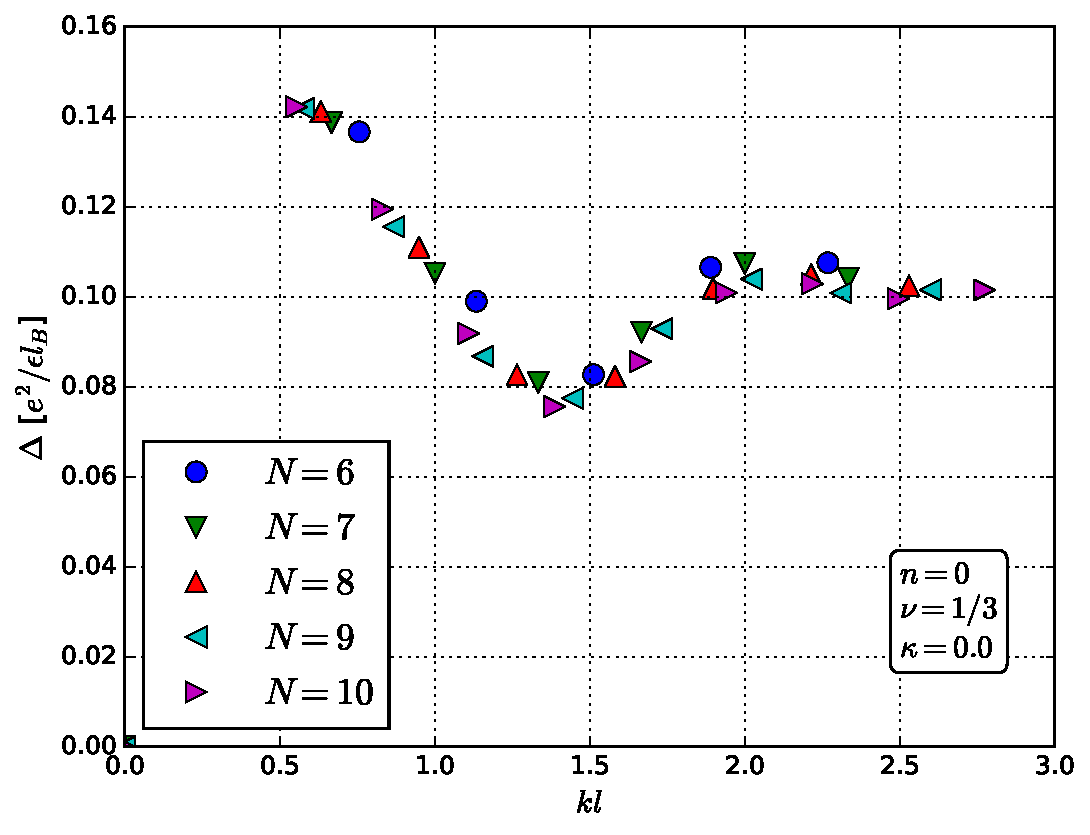
\includegraphics[width=10cm, angle=0]{ThesisCSULBLatexTemplate/figures/exc_disp_ns.pdf}
    \caption[The low energy CF-exciton dispersion broken down by system size.]{The low energy CF-exciton dispersion broken down by system size. We plot the exciton dispersion $\Delta$ for the bare Coulomb potential (LLM parameter $\kappa=0.0$) as a function of the wave vector $kl$ as calculated by the MC code for $6\leq N\leq10$ electrons at filling factor $\nu=1/3$ in the LLL ($n=0$).}
    \label{fig:exc_disp_ns} 
    \end{center}
    \end{figure}
    
    In Fig.~\ref{fig:exc_disp_kappas}, we plot the exciton dispersions produced by both MC and exact diagonalization for the benchmarks $6\leq N\leq10$ and $\kappa\in\{0.0,0.1,0.2\}$. As a general trend, the exciton dispersion shifts vertically downwards as a function of increasing $\kappa$ when calculated by exact diagonalization. This is expected since LLM effects reduce Haldane pseudopotentials (PPs) systematically and are expected to reduce all energies and energy gaps (see Sec.~\ref{ssec:apprEffPot}). The opposite trend, however, is observed when calculating the exciton dispersion via MC. The difference between these two trends is easier to see in Fig. \ref{fig:transp_gaps_vs_kappa}, where we plot just the transport gaps (calculated as the gap from the ground state energy to the lowest energy at the maximum total angular momentum state $L_{max}=N$) as a function of $\kappa$. The MC transport gaps increase with increasing $\kappa$, while the exact diagonalization benchmarks decrease with increasing $\kappa$. In the next section we discuss the sources of this error.
    
    \begin{figure}[H]
    \begin{center}
    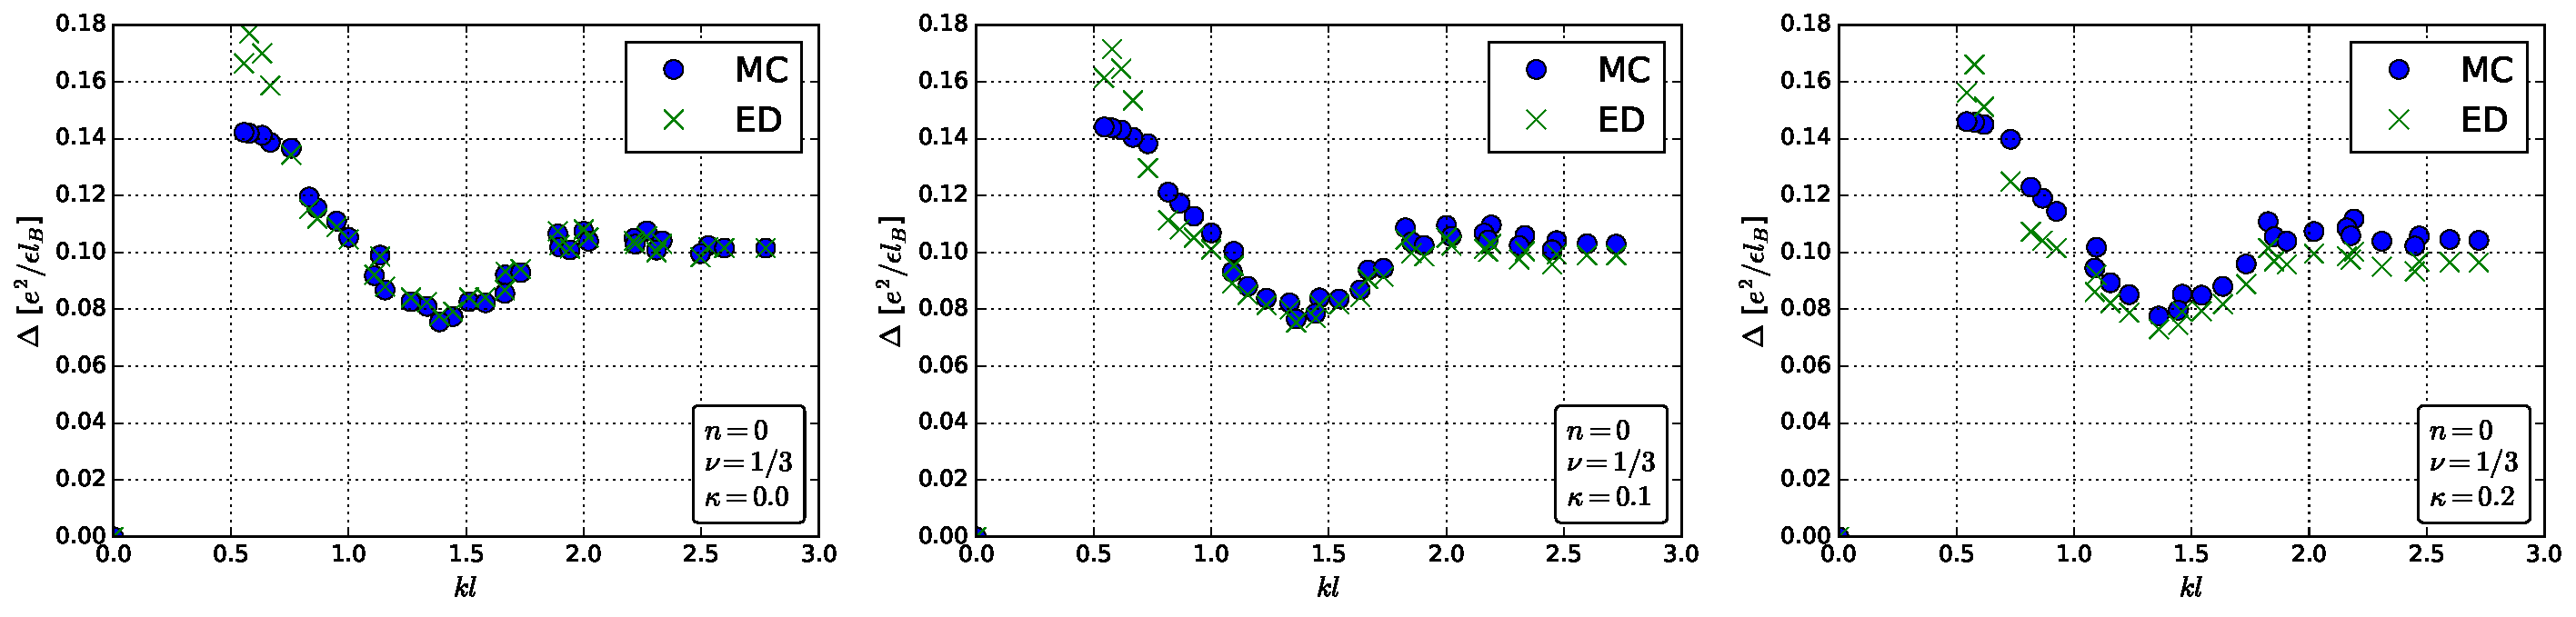
\includegraphics[width=10cm, angle=0,scale=1.5]{ThesisCSULBLatexTemplate/figures/exc_disp_kappas.pdf}
    \caption[The exciton dispersion benchmarks for different values of the LLM parameter.]{The exciton dispersion benchmarks for different values of the LLM parameter. The exciton ($\Delta$) dispersion as calculated by Monte Carlo (MC) and the exact diagonalization (ED) benchmarks is plotted as a function of the wave vector $kl$ in the LLL ($n=0$) for electron filling factor $\nu=1/3$ and $\kappa\in\{0.0,0.1,0.2\}$.}
    \label{fig:exc_disp_kappas} 
    \end{center}
    \end{figure}
    
    \begin{figure}[H]
    \begin{center}
    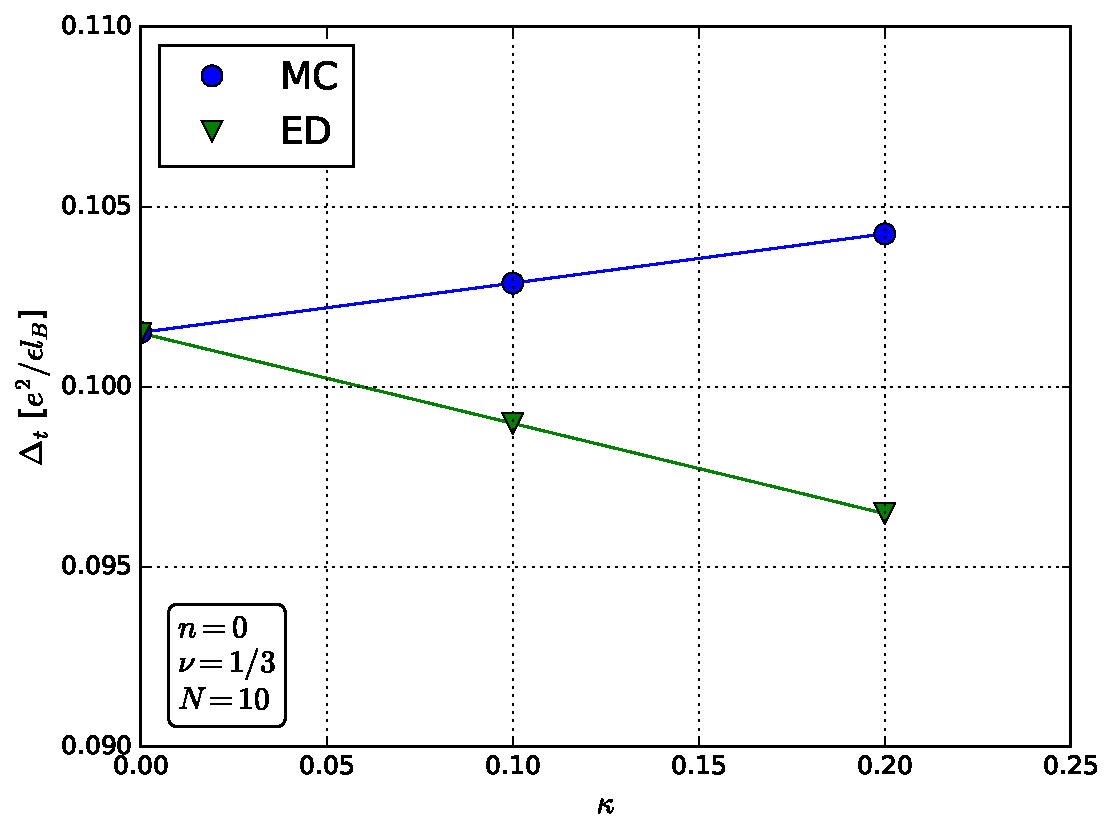
\includegraphics[width=10cm, angle=0]{ThesisCSULBLatexTemplate/figures/transp_gaps_vs_kappa.pdf}
    \caption[The transport gap benchmarks as a function of the LLM parameter.]{The transport gap benchmarks as a function of the LLM parameter. The constant approached at large wave vectors for a far separated CF-quasiparticle and CF-quasihole pair (transport gap $\Delta_t$) is plotted for $N=10$ electrons as a function of the LLM parameter $0.0\leq\kappa\leq0.2$ for Monte Carlo (MC) and the exact diagonalization (ED) benchmarks at filling factor $\nu=1/3$ in the LLL ($n=0$).}
    \label{fig:transp_gaps_vs_kappa}
    \end{center}
    \end{figure}
    
    \subsection{Sources of Error} \label{ssec:sourcErr}
    
    In the previous section, we used our method to calculate an exciton dispersion via MC and observed it had the opposite trend of the benchmark. We seek to explain this discrepancy in this section. In Fig. \ref{fig:transp_gaps_vs_kappa}, the MC transport gap matched comparatively well with the exact diagonalization transport gap for the bare Coulomb potential ($\kappa=0$). It then shifted vertically upward as $\kappa$ increased, in opposition to the benchmark. We believe this can be explained by looking at the configurations of electrons on the surface of the Haldane sphere which were accepted by the Metropolis-Hastings algorithm. 
    
    As mentioned in Secs.~\ref{ssec:montCarlInt} and~\ref{ssec:compFerm}, we start the MC code with electrons in a random configuration on the sphere, perturb each electron slightly in a random direction, and then calculate whether it is more likely to be in the perturbed (trial) configuration or the previous one. As mentioned in Sec.~\ref{ssec:compFermExcDisp}, we use the wavefunction for the lowest energy state at maximum total angular momentum ($L_{max}=N$) to calculate the probability of being in the trial or previous configuration. This means that if we were to plot a histogram representing the probability of each possible configuration getting accepted by the Metropolis-Hasting algorithm, it should closely resemble the pair correlation function of the CF wavefunction itself. This is designed so that the average energy of our accepted configurations (Eq.~\ref{metrAppr}, where $\mathcal{O}(\mathbf{R}^{(n)})=\sum_{i<j}V(|\mathbf{r}_i-\mathbf{r}_j|)$) quickly converges to the corresponding energy expectation value (Eq.~\ref{cfInt}) by sampling from the most likely states. 
    
    On the right side of Fig.~\ref{fig:r_sample_hist}, we plot a histogram representing the likelihood of each chord distance between two electrons on the sphere ($r=|\mathbf{r}_i-\mathbf{r}_j|$) being found in a configuration that was accepted by the Metropolis-Hastings algorithm. We can see in the figure that the distribution of the accepted distances has a strong negative skew. In other words, it does not represent a symmetric Gaussian distribution - the peak probability is skewed towards the larger values of $r$. This means that the CF wavefunction wants to, for the most part, keep the electrons as far away from each other as possible while still remaining on the sphere's surface. This behavior is expected since the wavefunction seeks to minimize the Coulomb energy of the electrons, which decreases as a function of their separation distance.
    
    On the left side of Fig.~\ref{fig:r_sample_hist}, we plot the difference between the effective real space potential and the bare Coulomb potential, $V_{eff}-V_{Coul}$ (see Sec.~\ref{ssec:apprEffPot}). This reflects the changes made to the Coulomb potential when incorporating LLM. We can see in the figure that at very small distances LLM decreases the potential, at mid-range distances it slightly increases it, and at far distances it has little to no effect. According to the histogram on the right side of the figure, the configurations where electrons are closer together, where LLM most affects the potential, are seldom accepted by the Metropolis-Hastings algorithm. It overwhelmingly samples from configurations where the particles are as far apart as possible and the Coulomb potential is mostly unchanged. To add to this, it samples more from the region of the histogram where $V_{eff}>V_{Coul}$ than it does from the region where $V_{eff}<V_{Coul}$, which explains why the transport gaps increase in the MC code with increasing $\kappa$ (please see Appendix~\hyperref[appendixB]{B} for more details on the behavior of the effective potential in real space).
    
    \begin{figure}[h]
    \begin{center}
    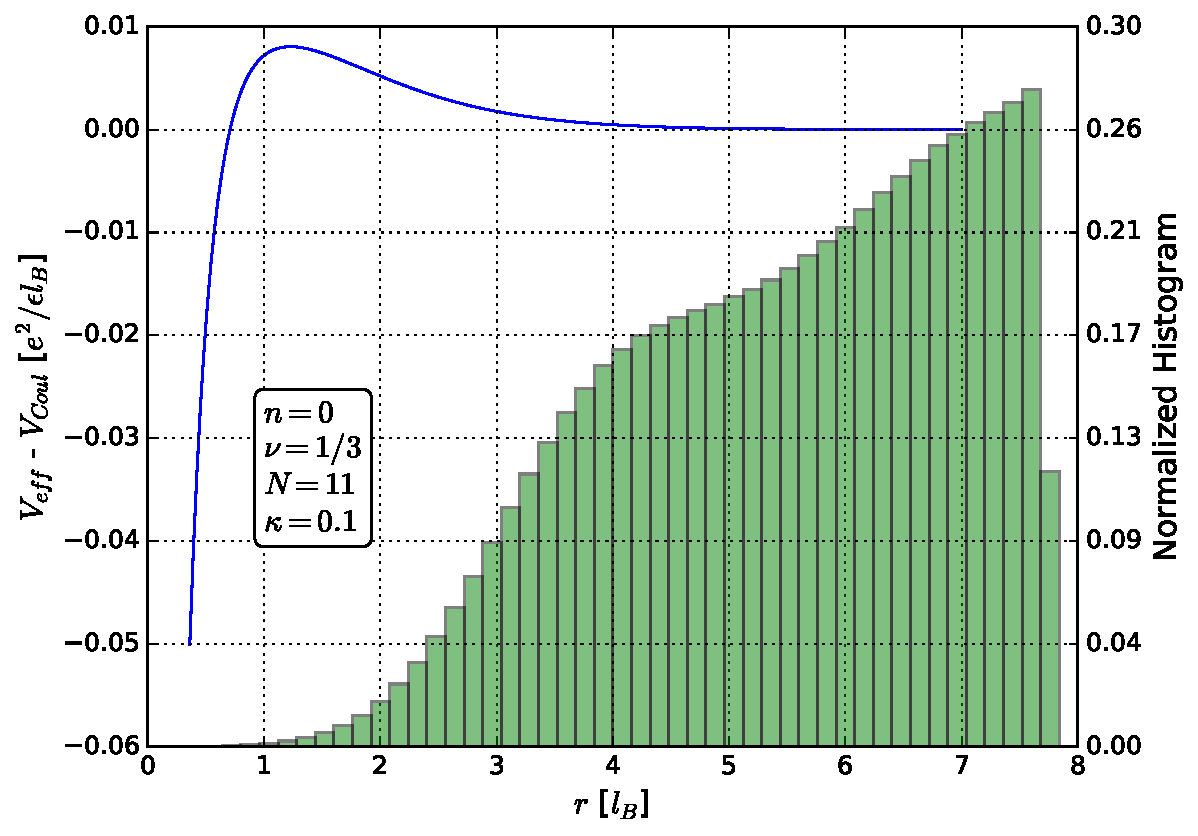
\includegraphics[width=10cm, angle=0]{ThesisCSULBLatexTemplate/figures/r_sample_hist.pdf}
    \caption[The potential difference due to LLM compared to the electron configurations accepted by the Metropolis-Hastings algorithm.]{The potential difference due to LLM compared to the electron configurations accepted by the Metropolis-Hastings algorithm. On the left vertical axis, we plot the difference between the LLM-incorporated modified Park potential and bare Coulomb potential $V_{eff}-V_{Coul}$ in real space as a function of the chord distance $r$ between electrons on the surface of the Haldane sphere. On the right vertical axis, we plot a normalized histogram showing the likelihood of a configuration with a chord distance $r$ being accepted by the Metropolis-Hastings algorithm. LLM most affects the configurations where electrons are closest together, but these are seldom accepted by the Metropolis-Hastings algorithm. This trial was done in the LLL ($n=0$) at filling factor $\nu=1/3$ for $N=11$ electrons and LLM parameter $\kappa=0.1$.}
    \label{fig:r_sample_hist} 
    \end{center}
    \end{figure}
    
    Several attempts were made to alleviate this systematic error. For our benchmarks, the radius of the Haldane sphere is fixed at $R=\sqrt{Q}l_B$ (see Sec.~\ref{sec:haldPseud}) with magnetic monopole strength $Q=3/2(N-1)$ (see Sec.~\ref{ssec:apprEffPotPar}). We cannot then, for example, bring the electrons closer together by decreasing the sphere's radius. Adding more electrons correspondingly increases the radius and spaces them out more. Increasing the number of iterations up to $10^9$ (as mentioned in Sec. \ref{sec:enExpVal}) made no significant difference to the accuracy of our simulations. We looked for a trend in the transport gap as a function of the number of iterations but this was not conclusive as the differences between trials with increased numbers of iterations were less than the standard error, which was comparatively very small. We also tried fine-tuning the ratio $\eta$, which determines whether a configuration will be accepted (see Sec.~\ref{ssec:compFerm}), to a constant value, but this did not provide consistent results across different systems. 
    
    We were inspired to try a technique called Laplace smoothing which is used to alleviate the zero frequency problem in the Naive Bayes model of machine learning \cite{kikuchi}. The idea behind our application of this was to artificially add an extra distance $r$ to each radius bin of the histogram so that the smallest radii were sampled $>0$ times while still trying to preserve the relative likelihood of the distances being sampled. In practice, we attempted this through multiple different initial conditions and behaviors for a variable number of pre-Metropolis-Hastings algorithm iterations. One example was starting with the electrons arranged in a circle very close to the north pole of the sphere, then accepting each configuration as they slowly moved down towards the equator before beginning the algorithm. We also tried starting with the electrons bunched close together on a line at the equator, accepting each step as they slowly spread out along the equator, and then starting the algorithm. We believe these methods produced large errors because we artificially inserted too many highly improbable states at too high of a frequency for the MC average energy to quickly converge to the energy expectation value.
    
    We were also inspired by work with quantum annealing \cite{finnila}. We tried implementing a parameter that described the number of MC iterations before a thermal fluctuation would reset the system to a random state. We believe that this method did not make any significant changes to our results because in practice the Metropolis-Hastings algorithm ended up being so good at finding equilibrium that it too quickly bypassed the less likely states where LLM was most affecting the real space potential. After adjusting every parameter in the MC code we could think of, we became closely acquainted with how sensitive our implementation of the Metropolis-Hastings algorithm is to changes made by the user. We conclude that the algorithm itself is not amenable to changes to which configurations are accepted, and therefore suggest further study be done to develop a new algorithm that can efficiently sample the configurations where realistic effects most change the real space potential so that MC estimates of FQH energies can be calculated in better agreement with experimental data collected in environments where effects often overlooked by theorists cannot be quenched.

\singlespacing

\chapter{CONCLUSION}\label{ch:conclusion}
\doublespacing

We developed a method for quickly incorporating realistic effects into Monte Carlo (MC) calculations of fractional quantum Hall (FQH) energy gaps. We applied our method to the effect Landau level mixing (LLM) at electron filling factor $\nu=1/3$ in the lowest Landau level (LLL) of graphene. We began by fitting a set of equations (Eqs.~\ref{eq:first_pp_corr} -~\ref{eq:last_pp_corr}) to data of two-body LLM Haldane pseudopotential (PP) corrections calculated by Arciniaga \textit{et al.} in Ref. \cite{arciniaga}. We perturbatively added (Eq.~\ref{potLlm}) these corrections to two-body PPs in the spherical geometry generated by applying the Wooten formula (Eq.~\ref{wootPpN0}) to the bare Coulomb potential. We chose a modified Park potential (Eq.~\ref{modPark}) as our effective real space potential, which contains parameters that allow it to be mapped via the Wooten formula to the aforementioned LLM-incorporated PPs. We generated a data set of these fitting parameters for magnetic monopole strengths $Q$ and LLM parameters $\kappa$ for the following systems of interest (see Sec.~\ref{ssec:apprEffPotPar}): $Q\in$ \{4.5, 6.0, 7.5, 9.0, 10.5, 12.0, 13.5, 15.0, 18.0, 22.5, 28.5, 36.0, 43.5, 58.5, 73.5\} and $\kappa\in$ \{0.0, 0.1, 0.2, 0.5, 0.8, 0.9, 2.2\}. We fit to this data equations (Eqs.~\ref{eqn:paramEq} -~\ref{eqn:lastPar}) for the parameters in terms of $\kappa$ and/or $Q$ so that the effective real space potential can be generated automatically by the MC code for each system. We used these approximated parameters to calculate the composite fermion (CF)-exciton dispersion in the MC code, which then prompted us to change the probability weight function used for acceptance sampling from the ground state wavefunction to the wavefunction of the lowest energy state at the maximum total angular momentum ($L_{max}=N$). We then benchmarked this dispersion against the result from exact diagonalization and found that the MC transport gaps increased with increasing $\kappa$, in opposition to the trend of the benchmark. We tried a number of different techniques to alleviate this problem but ultimately concluded that for a reasonable number of MC iterations, the states most affected by LLM are too improbable to be sampled at the relative frequency required by the Metropolis-Hastings algorithm. Future studies need to be done to develop an algorithm that will sample the less likely, more dense electron configurations so that realistic FQH energy gaps in graphene can be calculated in the thermodynamic limit as a function of $0.5<\kappa\leq2.2$ at $\nu\in$ \{1/3,2/5,3/7,4/9,5/11,...\}; eventually including three-body particle-hole symmetry breaking terms in higher LLs and novel effects in other materials.

\singlespacing

\clearpage
\vspace*{\fill} 
\begin{center}
\textbf{APPENDICES}
\end{center}
\vspace*{\fill}
\addcontentsline{toc}{chapter}{APPENDICES}
\clearpage

\addcontentsline{toc}{chapter}{\hspace*{2em}\thechapter. USER-DEFINED PYTHON FUNCTIONS}
\clearpage
\doublespacing
\vspace*{\fill} 
\begin{center}
\textbf{APPENDIX A}\label{appendixA}\\
\medskip
\textbf{USER-DEFINED PYTHON FUNCTIONS}\\
\end{center}
\vspace{7pt}
\vspace*{\fill}
\singlespacing
\chapter*{} % Left blank for no section headers
\addtocounter{chapter}{1}
\setcounter{chapter}{1}% Equivalent to "letter A"
\renewcommand{\thechapter}{\Alph{chapter}}%
\doublespacing

\begin{lstlisting}[language=Python]
import pandas as pd
import numpy as np
from typing import Tuple, List
from scipy.optimize import curve_fit, root
import scipy.integrate as integrate
from scipy.special import eval_legendre
from sympy import N, symbols, solve, exp
from sympy.physics.wigner import wigner_3j, wigner_6j

def vEff(r: float, prms: Tuple[float]) -> float:
    """Return the two-body real space effective potential."""
    
    b1, b2, beta1, beta2 = prms
    
    return 1/r + b1*np.exp(-beta1*r) + b2*r**2*np.exp(-beta2*r)
    
def vK(k: int, prms: Tuple[float]) -> float:
    """Return the V_k term of Wooten's formula for mapping a two-body, real space effective potential
    to a Haldane pseudopotential."""
    
    coeff = (2*k+1)/2
    integ = integrate.quad(lambda x: vEff(np.sqrt(2*(1-x)), prms)*eval_legendre(k, x), -1, 1)
    
    return coeff*integ[0]

def wootenPP(qL: Tuple[float], prms: Tuple[float]) -> float:
    """Return the value of the effective potential that has been mapped
    to a Haldane pseudopotential via the Wooten formula."""
    
    q, l = qL
    
    coeff = (-1)**(2*q+l) * (2*q+1)**2/np.sqrt(q)
    
    # save terms in the sum as a list to be summed over
    sumTerms = []
    for k in range(int(2*q+1)):
        # in the lowest Landau level l = Q
        sumTerms.append(
               vK(k, prms)*N(wigner_6j(l, q, q, k, q, q))*N(wigner_3j(q, k, q, -q, 0, q))**2)
    
    return coeff*sum(sumTerms)
    
def findRootWootenPP(prms: Tuple[float], args: List[float]) -> List[float]:
    """Return the difference between the Coulomb and Landau level mixing-incorporated Haldane pseudopotentials
    for the first nPrms odd m values so a root finding method can solve for the fitting parameters."""
    
    # need as many equations as there are parameters
    nPrms = len(prms)
    
    # args input is [q, kappa, deltas[0:nPrms]]
    q, kappa, deltas = args[0], args[1], args[2:nPrms+2]

    res = []
    for i in range(nPrms):
        
        # m odd
        m = 2*i+1
        
        # L = 2Q-m in the lowest LL
        qL = (q, 2*q-m)
        
        # Coulomb parameters
        prms0 = ()
        for j in range(nPrms):
            prms0 = prms0 + (0.0,)
        
        # V_eff = V_Coulomb + kdV
        llmPP = wootenPP(qL, prms0) + kappa * deltas[i]
        
        res.append(wootenPP(qL, prms) - llmPP)
    
    return res
    
def fittingPrms(args: List[float], prms0: Tuple[float]) -> Tuple[float]:
    """Return the parameters that fit the effective potential to the Landau level mixing-incorporated Haldane
    pseudopotential data."""
    
    # need as many equations as there are parameters
    nPrms = len(prms0)
    
    # args input is [q, kappa, deltas[0:nPrms]]
    q, kappa, deltas = args[0], args[1], args[2:nPrms+2]

    # find roots
    sol = root(findRootWootenPP, prms0, args=(args), method='hybr')
    
    return tuple(sol.x)
    
def vqlDF(q: float, kappa: float, prms: Tuple[float]) -> pd.DataFrame:
    """Return a DataFrame containing the fitted Landau level mixing-incorporated Haldane pseudopotentials as a 
    function of the single-particle relative angular momentum in the spherical geometry L."""

    # need as many equations as there are parameters
    nPrms = len(prms)
    
    # m can be any odd value up to 2Q in the lowest LL
    mArray = list( range(1, int(2*q + 1), 2) )
    
    # generate PPs from fitted Park parameters
    data = []
    for m in mArray:
        # L = 2Q - m in the lowest LL
        qL = (q, 2*q - m)
        data.append([qL[1], wootenPP(qL, prms)])
    
    # put in order of increasing L
    data.reverse()
    
    return pd.DataFrame(data, columns = ['L', 'V_Q(L)'])
    
def b12Func(qKappa: Tuple[float], c1: float, c2: float, c3: float) -> float:
    """Return the value of the Landau Level mixing-incorporated Haldane pseudopotential parameter function 
    b_i(Q, kappa)."""
    
    q, kappa = qKappa
    
    return (c1*q**c2 + c3)*kappa
    
def b_fun_prms(dfPrms: pd.DataFrame, prms0: List[float], b1: bool=False, b2: bool=False) -> np.ndarray:
    """Return the parameters c_i for the Landau Level mixing-incorporated Haldane pseudopotential parameter function 
    b_i(Q, kappa)."""
    
    try:
        if b1 and not b2:
            col = 'b1'
        elif b2 and not b1:
            col = 'b2'
        else:
            raise ValueError

        # make DataFrame of values for Q>6 since the fit will be more accurate and we are interested in the therm lim
        dfTemp = dfPrms.query('(Q > 6.0) & (kappa > 0.0)')
        dfTemp.reset_index(drop=True, inplace=True)

        x = ( dfTemp['Q'].to_list(), dfTemp['kappa'].to_list() )
        y = dfTemp[col].to_list()

        prms, pcov = curve_fit(b12Func, x, y, prms0)
        
        return prms

    except ValueError:
        return 'ValueError: please input \'b1=True\' xor \'b2=True\'.'
        
def beta12Func(q: float, c1: float, c2: float, c3: float) -> float:
    """Return the value of the Landau Level mixing-incorporated Haldane pseudopotential parameter function
    beta_i(Q, kappa)."""
    
    return c1*q**c2 + c3
    
def beta_fun_prms(dfPrms: pd.DataFrame, prms0: List[float], beta1: bool=False, beta2: bool=False) -> np.ndarray:
    """Return the parameters c_i for the Landau Level mixing-incorporated Haldane pseudopotential parameter function
    beta_i(Q, kappa)."""
    
    try:
        if beta1 and not beta2:
            col = 'beta1'
        elif beta2 and not beta1:
            col = 'beta2'
        else:
            raise ValueError

        # make DataFrame of values for Q>6 since the fit will be more accurate and we are interested in the therm lim
        dfTemp = dfPrms.query('(Q > 6.0) & (kappa > 0.0)')
        dfTemp.reset_index(drop=True, inplace=True)

        x = dfTemp['Q'].to_list()
        y = dfTemp[col].to_list()

        prms, pcov = curve_fit(beta12Func, x, y, prms0)
        return prms

    except ValueError:
        return 'ValueError: please input \'beta1=True\' xor \'beta2=True\'.'
        
def rangeFunc(n, c1, c2, c3):
    """Return the RANGE value."""
    
    res = c1*n**c2 + c3
    
    return res
\end{lstlisting}
    
\singlespacing

\clearpage
\doublespacing
\vspace*{\fill} 
\begin{center}
\textbf{APPENDIX B}\label{appendixB}\\
\medskip
\textbf{REAL SPACE EFFECTIVE POTENTIAL}\\
\end{center}
\vspace{7pt}
\vspace*{\fill}
\singlespacing
\addcontentsline{toc}{chapter}{\hspace*{2em}\thechapter. REAL SPACE EFFECTIVE POTENTIAL}
\chapter*{} % Left blank for no section headers
\addtocounter{chapter}{1}
\doublespacing

Looking at the plot of the difference between the two-body effective potential and the bare Coulomb potential ($V_{eff}-V_{Coul}$) in real space as a function of the chord distance $r$ between electrons on the Haldane sphere in Fig. \ref{fig:exc_disp_kappas}, we see that the magnitude of the difference at any distance for magnetic monopole strength $Q=7.5$ increases with increasing Landau level mixing (LLM) parameter $\kappa$. We also notice that the differences for every $\kappa$ value intersect at $V_{eff}-V_{Coul}=0$, or $V_{eff}=V_{Coul}$, for $r\approx0.8$. In this Appendix, we want to explain the cause of this and understand how this difference changes as a function of $Q$. 

From the modified Park potential (Eq. \ref{modPark}), we have
\begin{equation}\label{potDiff}
  V_{eff}-V_{Coul}=b_1e^{-\beta_1r}+b_2r^2e^{-\beta_2r}. 
\end{equation}
We can solve for the distance at which the effective potential intersects the Coulomb potential, $r(V_{eff}=V_{Coul})$, by setting the left side of the equation above to 0 and solving for $r$. This expression depends linearly on $b_i$ which depend linearly on $\kappa$, and on $\beta_i$ which do not depend on $\kappa$, so the $\kappa$ dependence of $r(V_{eff}=V_{Coul})$ is cancelled out. We used the Python library SymPy so solve for the unique solutions of $r(V_{eff}=V_{Coul})$ \cite{sympy}, 
\begin{equation}\label{r_v_eff_eq_v_coul}
\left[\frac{2 W\left(\frac{\sqrt{-\frac{b_{1}}{b_{2}}}\left(-\beta_{1}+\beta_{2}\right)}{2}\right)}{\beta_{1}-\beta_{2}}, \frac{2 W\left(\frac{\sqrt{-\frac{b_{1}}{b_{2}}}\left(\beta_{1}-\beta_{2}\right)}{2}\right)}{\beta_{1}-\beta_{2}}\right],
\end{equation}
where $W$ is the Lambert W function. We can use the following sample parameter values to determine which expression to use: $b_1(7.5, 2.2)=-6.879503$, $b_2(7.5, 2.2)=1.105104$, $\beta_1(7.5)=4.485793$ and $\beta_2(7.5)=1.468513$. Since $\beta_1>\beta_2$, we have 
\begin{equation}\label{r_v_eff_eq_v_coul_singl}
r(V_{eff}=V_{Coul})=\frac{2}{\beta_1-\beta_2}W\left(\frac{\beta_1-\beta_2}{2}\sqrt{\frac{-b_1}{b_2}}\right).
\end{equation}
We can plug in the sample parameter values to find $r(V_{eff}=V_{Coul},7.5)=0.774999$. The full expression of the distance where the effective potential intersects the Coulomb potential in real space as a function of $Q$ is as follows:
\begin{equation}
    \resizebox{\textwidth}{!}
     {
        r(V_{eff}=V_{Coul},Q)=\frac{2 W\left(\sqrt { \frac { Q ^ { 0 . 4 5 2 2 1 6} + 0 . 2 4 1 2 4 6} { 1 . 8 4 7 2 3 7 \cdot 1 0 ^ { - 5 } Q ^ { 2. 2 7 4 2 2 6} + 0 . 0 4 8 4 2 6} } \left(0.153363 Q^{0.537208}-0.005767 Q^{1.150906}+0.116654\right)\right)}{0.906035 Q^{0.537207}-0.034071 Q^{1.151906}+0.689167}.
     }
\end{equation}

We can view the behavior of $r(V_{eff}=V_{Coul},Q)$ in the plot in Fig. \ref{fig:r_vEff_eq_vCoul_vs_q}. It starts to diverge near $Q\approx253.5$, which corresponds to $N=169$ electrons at filling factor $\nu=1/3$ in the lowest Landau level (LLL). It appears that for $Q\geq253.5$, $V_{eff}$ starts below $V_{Coul}$, then quickly converges to it from below without ever rising above (for $Q=252.0$, $V_{eff}$ is within 1\% of $V_{Coul}$ for all points $r\gtrsim0.345$). We confirm this behavior of the difference with respect to $Q$ in the plot in Fig. \ref{fig:vEff_minus_vCoul_vs_r_qs}.

\begin{figure}[H]
\begin{center}
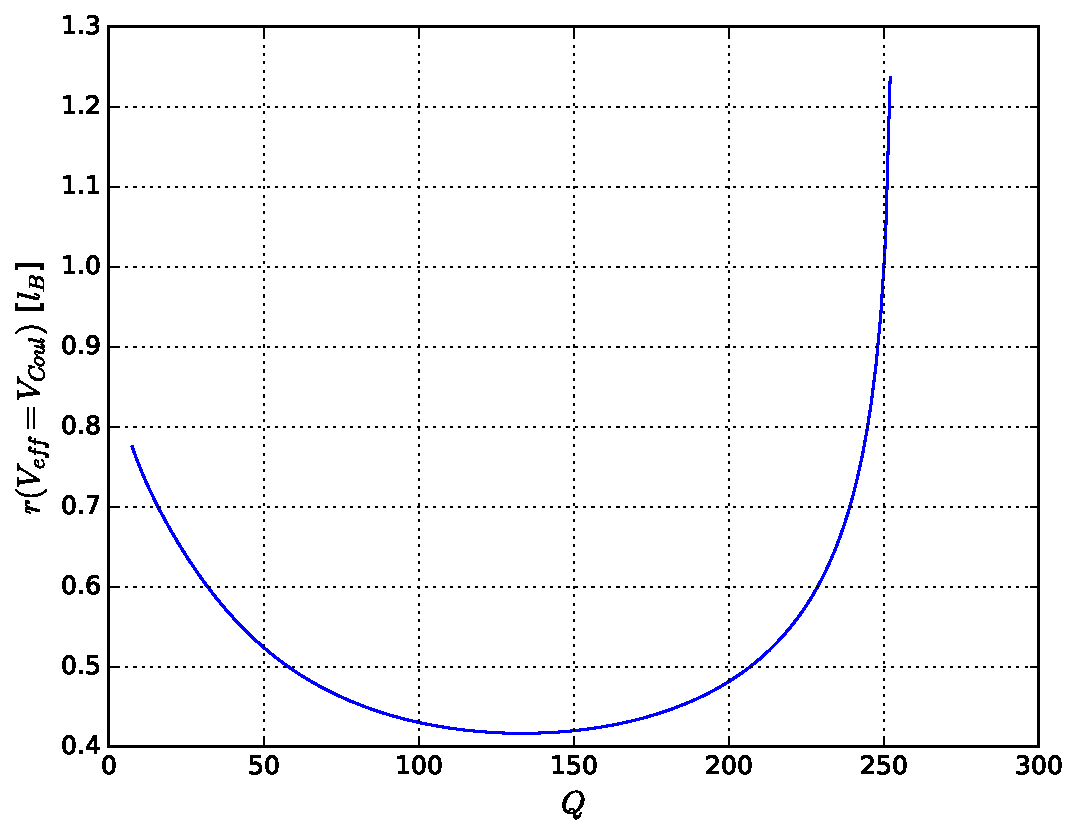
\includegraphics[width=10cm, angle=0]{ThesisCSULBLatexTemplate/figures/r_vEff_eq_vCoul_vs_q.pdf}
\caption[The chord distance between electrons on the Haldane sphere where the effective potential intersects the bare Coulomb potential in real space for all LLM parameter values.]{The chord distance between electrons on the Haldane sphere where the effective potential intersects the bare Coulomb potential in real space for all LLM parameter values. We plot $r(V_{eff}=V_{Coul})$ as a function of the magnetic monopole strength $Q$ from data collected in the LLL with filling factor $\nu=1/3$. It diverges near $Q\approx253.5$.}
\label{fig:r_vEff_eq_vCoul_vs_q} 
\end{center}
\end{figure}

\begin{figure}[p]
\begin{center}
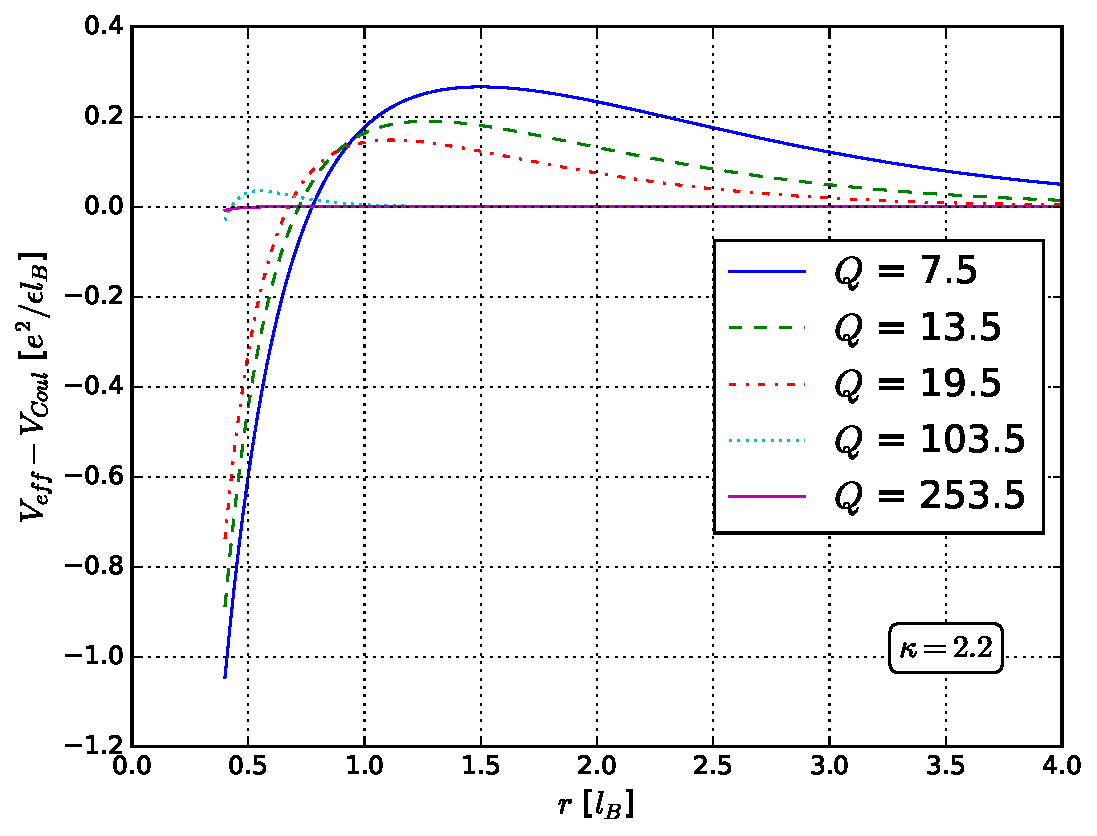
\includegraphics[width=10cm, angle=0]{ThesisCSULBLatexTemplate/figures/vEff_minus_vCoul_vs_r_qs.pdf}
\caption[The difference between the effective potential and bare Coulomb potential in real space at different magnetic monopole strengths.]{The difference between the effective potential and bare Coulomb potential in real space at different magnetic monopole strengths.We plot $V_{eff}-V_{Coul}$ as a function of the chord distance between electrons on the Haldane sphere $r$ in the LLL at filling factor $\nu=1/3$, LLM parameter $\kappa=2.2$, and $Q\in\{7.5,13.5,19.5,103.5,253.5\}$. For smaller values of $Q$, the difference is negative at small distances, then positive at larger differences before converging to zero at far distances. When $Q\gtrsim253.5$, the difference quickly converges to 0 from below without ever reaching positive values.}
\label{fig:vEff_minus_vCoul_vs_r_qs} 
\end{center}
\end{figure}

\singlespacing

\clearpage
\doublespacing
\vspace*{\fill} 
\begin{center}
\textbf{APPENDIX C}\label{appendixC}\\
\medskip
\textbf{MONTE CARLO RANGE VALUES}\\
\end{center}
\vspace{7pt}
\vspace*{\fill}
\singlespacing
\addcontentsline{toc}{chapter}{\hspace*{2em}\thechapter. MONTE CARLO RANGE VALUES}
\chapter*{} % Left blank for no section headers
\addtocounter{chapter}{1}
\doublespacing

In the Monte Carlo (MC) code, the \texttt{RANGE} value determines the ratio with which the steps of the Metropolis-Hastings algorithm (see Sec.~\ref{ssec:compFerm}) are accepted, which is ideally $\approx50\%$ \cite{jain}. We used Hernandez's data from Appendix A of Ref. \cite{uriel} to fit the parameters for the \texttt{RANGE} values that correspond to a $50\%$ acceptance ratio as a function of the number of electrons $N$ at filling factor $\nu=1/3$ in the lowest Landau level (LLL). In our computational experiments, these \texttt{RANGE} values seemed to produce similar results for $\nu\in\{2/5,3/7,4/9,5/11,...\}$, but further study needs to be done to determine quantitatively how accurate this formula is at other filling factors. The equation of best fit,
\begin{equation}\label{range}
\texttt{RANGE}(N)=1.211910N^{−1.419258}+0.018149,
\end{equation}
is plotted along with the data from Ref. \cite{uriel} in Fig. \ref{fig:range_vs_n}.

\begin{figure}[H]
\begin{center}
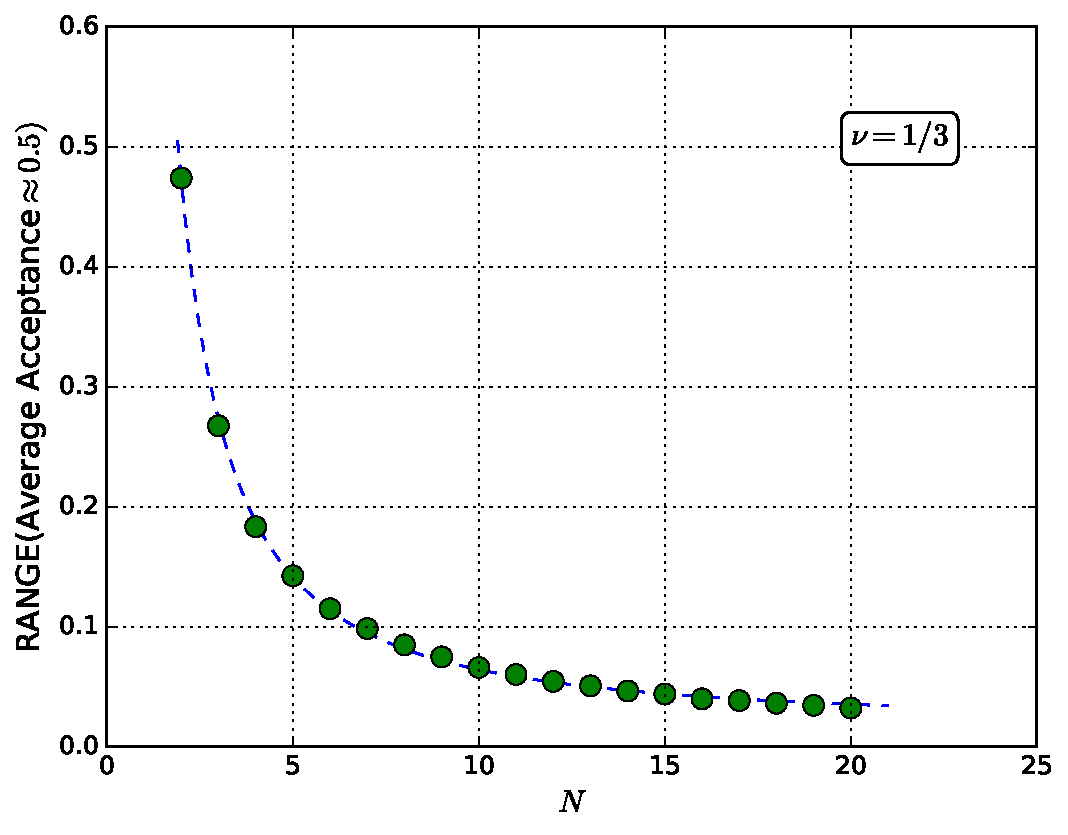
\includegraphics[width=10cm, angle=0]{ThesisCSULBLatexTemplate/figures/range_vs_n.pdf}
\caption[Monte Carlo \texttt{RANGE} values.]{Monte Carlo \texttt{RANGE} values. The equation of best fit for the \textt{RANGE} values that produced a 50\% acceptance ratio in the Monte Carlo code are plotted as a function of the number of electrons $N$ at filling factor $\nu=1/3$ in the LLL.}
\label{fig:range_vs_n} 
\end{center}
\end{figure}

\singlespacing

\renewcommand{\bibname}{References}

\clearpage
\addcontentsline{toc}{chapter}{REFERENCES}
\vspace*{\fill} 
\centering 
\textbf{REFERENCES}
\vspace*{\fill}
\clearpage

\doublespacing
\printbibliography


\end{document}
